\documentclass[a4paper,onecolumn,unpublished]{quantumarticle}
\pdfoutput=1

% ==================== BEGIN preamble.tex ====================
\usepackage[utf8]{inputenc}
\usepackage[T1]{fontenc}
\usepackage{lmodern,microtype}
\usepackage{amsmath,amssymb,amsthm,graphicx}
\usepackage{xcolor,array,bm,braket,tikz-cd}
\usetikzlibrary{knots,decorations.markings}
\tikzstyle directed=[postaction={decorate,decoration={markings,mark=at position #1 with {\arrow{>}}}}]
\tikzstyle rdirected=[postaction={decorate,decoration={markings,mark=at position #1 with {\arrow{<}}}}]
\usepackage[all]{xy}
\usepackage{caption,subcaption,ragged2e}
\usepackage[numbers,sort&compress]{natbib}
\usepackage[colorlinks=true,linkcolor=blue,citecolor=blue,urlcolor=blue]{hyperref}
\usepackage{schmidhuber}
\usepackage{nicefrac,xfrac,wrapfig,physics}
% Keep our probability operator instead of physics' automatic argument parser.
\let\Pr\relax
\DeclareMathOperator*{\Pr}{\mathbf{Pr}}
\setlength{\emergencystretch}{1.5em}

% ==================== BEGIN diagram-macros.tex ====================
\theoremstyle{plain}
\newtheorem{theorem}{Theorem}
\newtheorem{theorem_noname}{Theorem}
\newtheorem{corollary}[theorem]{Corollary}
\newtheorem{proposition}[theorem]{Proposition}
\newtheorem{lemma}[theorem]{Lemma}
\newtheorem{algorithm}[theorem]{Algorithm}
\newtheorem{axiom}[theorem]{Axiom}
\newtheorem{claim}[theorem]{Claim}
\newtheorem{conclusion}[theorem]{Conclusion}
\newtheorem{notation}[theorem]{Notation}
\newtheorem{summary}[theorem]{Summary}
\theoremstyle{definition}
\newtheorem{example}[theorem]{Example}
\newtheorem{definition}[theorem]{Definition}
\newtheorem{conjecture}[theorem]{Conjecture}
\theoremstyle{definition}
\newtheorem{remark}[theorem]{Remark}
\newtheorem{acknowledgement}[theorem]{Acknowledgement}

\numberwithin{equation}{section}
\renewcommand*{\theHequation}{\theHsection.\arabic{equation}}


 
\providecommand{\AL}[1]{{\color{orange}\textbf{AL:} #1}}


\newcommand{\hackcenter}[1]{
 \xy (0,0)*{#1}; \endxy}

 \usepackage{bbm}
 \def\1{\mathbbm{1}}%
\newcommand{\maps}{\colon}

 
            
\newcommand{\Ker}{\text{Ker }}
\newcommand{\Ima}{\text{Im }}
\newcommand{\bigO}{$\mathcal{O}$}
\newcommand{\tens}{\otimes}
\newcommand{\id}{\mathbb{1}}
\newcommand{\lagr}{\mathcal{L}}
\newcommand{\dt}{\frac{d}{dt}}
\newcommand{\dif}[2]{\frac{\partial#1}{\partial#2}}
\newcommand{\hal}{\mathcal{H}}
\newcommand{\del}{\partial}
\newcommand{\x}{\textbf{x}}
\newcommand{\bigu}{\mathcal{U}}
\newcommand{\bigslant}[2]{{\raisebox{.2em}{#1}\left/\raisebox{-.2em}{#2}\right.}}
\newcommand{\homk}{\textbf{$H_k$}}
\renewcommand{\to}{\rightarrow}


\newcommand{\sphere}[1][1]{
\xy
(0,0)*{
\begin{tikzpicture} [fill opacity=0.2, scale=#1]
	\path [fill=black] (0,0) circle (1);
	\draw (-1,0) .. controls (-1,-.4) and (1,-.4) .. (1,0);
	\draw[dashed] (-1,0) .. controls (-1,.4) and (1,.4) .. (1,0);
	\draw[very thick] (0,0) circle (1);
\end{tikzpicture}};
\endxy}
 



\newcommand{\und}{\underline}


\makeatletter
\DeclareFontFamily{OMX}{MnSymbolE}{}
\DeclareSymbolFont{MnLargeSymbols}{OMX}{MnSymbolE}{m}{n}
\SetSymbolFont{MnLargeSymbols}{bold}{OMX}{MnSymbolE}{b}{n}
\DeclareFontShape{OMX}{MnSymbolE}{m}{n}{
    <-6>  MnSymbolE5
   <6-7>  MnSymbolE6
   <7-8>  MnSymbolE7
   <8-9>  MnSymbolE8
   <9-10> MnSymbolE9
  <10-12> MnSymbolE10
  <12->   MnSymbolE12
}{}
\DeclareFontShape{OMX}{MnSymbolE}{b}{n}{
    <-6>  MnSymbolE-Bold5
   <6-7>  MnSymbolE-Bold6
   <7-8>  MnSymbolE-Bold7
   <8-9>  MnSymbolE-Bold8
   <9-10> MnSymbolE-Bold9
  <10-12> MnSymbolE-Bold10
  <12->   MnSymbolE-Bold12
}{}

\let\llangle\@undefined
\let\rrangle\@undefined
\DeclareMathDelimiter{\llangle}{\mathopen}%
                     {MnLargeSymbols}{'164}{MnLargeSymbols}{'164}
\DeclareMathDelimiter{\rrangle}{\mathclose}%
                     {MnLargeSymbols}{'171}{MnLargeSymbols}{'171}

\usepackage{pict2e}

\makeatletter

\newcommand*\@KP@Large@frame[2]{%
    \setlength\unitlength{\fontdimen 22 #1\tw@}%
    \vrule \@width\z@ \@height 4\unitlength \@depth\tw@\unitlength
    \begin{picture}(6,2)(-3,-1)%
        \def\@KP@Radius     {3}%
        \def\@KP@Hole@radius{.5}% The same value seem adequate for both...
        \def\@KP@Diameter   {6}%
        #2%
    \end{picture}%
}
\newcommand*\@KP@Small@frame[2]{%
    \setlength\unitlength{\fontdimen 22 #1\tw@}%
    \vrule \@width\z@ \@height \thr@@\unitlength \@depth\@ne\unitlength
    \begin{picture}(4,2)(-2,-1)%
        \def\@KP@Radius     {2}%
        \def\@KP@Hole@radius{.5}% ... but let it be customizable too.
        \def\@KP@Diameter   {4}%
        #2%
    \end{picture}%
}

\newcommand*\@KP@Radius     {}
\newcommand*\@KP@Hole@radius{}
\newcommand*\@KP@Diameter   {}
\newcommand*\@KP@Shape@A{%
    \put(0,0){\circle{\@KP@Diameter}}%
}
\newcommand*\@KP@Shape@B{%
    \Line(-\@KP@Radius,\@KP@Radius )(\@KP@Radius,-\@KP@Radius)%
    \Line(-\@KP@Radius,-\@KP@Radius)(-\@KP@Hole@radius,-\@KP@Hole@radius)%
    \Line(\@KP@Radius ,\@KP@Radius )(\@KP@Hole@radius ,\@KP@Hole@radius )%
}
\newcommand*\@KP@Shape@C{%
    \cbezier(-\@KP@Radius,\@KP@Radius )(0,0)(0,0)(\@KP@Radius,\@KP@Radius )%
    \cbezier(-\@KP@Radius,-\@KP@Radius)(0,0)(0,0)(\@KP@Radius,-\@KP@Radius)%
}
\newcommand*\@KP@Shape@D{%
    \cbezier(-\@KP@Radius,-\@KP@Radius)(0,0)(0,0)(-\@KP@Radius,\@KP@Radius)%
    \cbezier(\@KP@Radius ,-\@KP@Radius)(0,0)(0,0)(\@KP@Radius ,\@KP@Radius)%
}

\newcommand*\@KP@Atomic@mathpalette[1]{%
    \mathinner{% or "\mathord"?
        \mathchoice{%
            \linethickness{.6\p@}% Tip: use thicker lines if you decide to 
            \@KP@Large@frame \textfont {#1}%
        }{%
            \linethickness{.4\p@}% adjustable
            \@KP@Small@frame \textfont {#1}%
        }{%
            \linethickness{.3\p@}% adjustable
            \@KP@Small@frame \scriptfont {#1}%
        }{%
            \linethickness{.2\p@}% adjustable
            \@KP@Small@frame \scriptscriptfont {#1}%
        }%
    }%
}

\newcommand*\KPA{\@KP@Atomic@mathpalette \@KP@Shape@A}
\newcommand*\KPB{\@KP@Atomic@mathpalette \@KP@Shape@B}
\newcommand*\KPC{\@KP@Atomic@mathpalette \@KP@Shape@C}
\newcommand*\KPD{\@KP@Atomic@mathpalette \@KP@Shape@D}

\makeatother
% ===================== END diagram-macros.tex =====================

% ===================== END preamble.tex =====================

\begin{document}
\title{Quantum computing and Khovanov homology}

% ==================== BEGIN authors.tex ====================
\author{Alexander Schmidhuber}
\email{alexsc@mit.edu}
\affiliation{Center for Theoretical Physics, Massachusetts Institute of Technology, Cambridge, MA 02139}

\author{Michele Reilly}
\affiliation{Department of Mechanical Engineering, Massachusetts Institute of Technology, Cambridge, MA 02139}

\author{Paolo Zanardi}
\affiliation{Department of Physics, University of Southern California, Los Angeles, CA 90007}
\affiliation{Department of Mathematics, University of Southern California, Los Angeles, CA 90007}

\author{Seth Lloyd}
\affiliation{Department of Mechanical Engineering, Massachusetts Institute of Technology, Cambridge, MA 02139}

\author{Aaron Lauda}
\email{lauda@usc.edu}
\affiliation{Department of Mathematics, University of Southern California, Los Angeles, CA 90007}
\affiliation{Department of Physics, University of Southern California, Los Angeles, CA 90007}


\date{}
% ===================== END authors.tex =====================

\begin{abstract}
Khovanov homology is a powerful knot invariant that categorifies the Jones polynomial, detects the unknot, and has proposed realizations in supersymmetric gauge theory. Yet, its computational complexity remains poorly understood. This work gives a self-contained introduction to Khovanov homology and examines quantum algorithms for its complex Betti numbers. We encode these numbers as zero-energy subspace dimensions of a Hodge Laplacian, give sparse access to its Hermitian differential, and describe projection onto the harmonic subspace via quantum phase estimation.

The algorithm's efficiency depends on the spectral gap of the Laplacian and the ability to efficiently prepare a guiding state with sufficient overlap with its ground space. We give a conditional procedure for exact Betti-number estimation, specifying the required Gibbs-state accuracy and sampling costs, including their dependence on the Betti number. Numerical computation on fixed diagrams reveals substantial variation in the observed gaps. The class of alternating knots, however, appears more structured, with observed minima agreeing with exact bidegree formulas over the tested range through thirteen crossings. We examine a guiding state derived via the spanning-tree model of Khovanov homology, which has a smaller chain space while containing the same homology. For connected alternating diagrams, uniform tree sampling yields an efficient classical algorithm for additively approximating the normalized reduced Betti numbers. We complement our algorithmic framework with complexity-theoretic results showing that additive approximations at the corresponding Jones-polynomial normalization scales are \(\DQC\)-hard and \(\BQP\)-hard, and that exact computation is \(\sharpP\)-hard.
\end{abstract}
\maketitle

% ==================== BEGIN introduction.tex ====================
\section{Introduction}
Low-dimensional topology has long served as a useful testing ground for identifying problems where quantum algorithms offer a genuine advantage over classical approaches.  
 A central example is the Jones polynomial, whose additive approximation at certain roots of unity is universal for quantum computation \cite{freedman2002simulation,Aharonov-Jones-Landau}.

In this work, we focus on quantum algorithms for a more general topological invariant, called \emph{Khovanov homology}, which is a \textit{categorification} of the Jones polynomial.  
\smallskip 

\noindent \textbf{Jones polynomial and topological quantum field theory.} 
The Jones polynomial \cite{jones1997polynomial} is a topological invariant associated with knots and links in 3-dimensional space.  This polynomial does not change under continuous deformations of a knot and can thereby be used to distinguish different knots. As a computational problem, exact evaluation of the Jones polynomial is $\sharpP$-hard in general, and sufficiently accurate approximation is hard in several regimes~\cite{kuperberg2015hard}.  At certain roots of unity, however, \emph{quantum} algorithms produce natural additive approximations in polynomial time~\cite{Aharonov-Jones-Landau}.
The error scale depends on the diagram presentation. For plat closures of braids with the polynomial parameter specialized to a fifth root of unity, an algorithm that can approximate the Jones polynomial at the specified normalization can simulate any computation that a quantum computer can perform efficiently; this approximation problem is $\BQP$-complete~\cite{FreedmanLarsenWang2002,aharonov2011bqp}.   

One compelling explanation for why the Jones polynomial is so amenable to quantum algorithms is Witten's work showing that the Jones polynomial has a physical incarnation as observables associated to Wilson loops in 3D Chern--Simons theory~\cite{Witten-Jones}. This physical interpretation of the Jones polynomial within topological quantum field theory has also led to advances in low-dimensional topology and the study of 3-manifolds~\cite{MR1091619}, integrable systems and the theory of quantum groups~\cite{Kauff,Jones-stat}, and
inspired new approaches to quantum computing, such as topological quantum computation~\cite{FKLW,Kitaev}, which leverages the topological nature of these theories to develop naturally error-resistant quantum computational schemes.  
\smallskip 

\noindent \textbf{Khovanov homology and categorification.}   Nearly two decades after the discovery of the Jones polynomial, Mikhail Khovanov realized that it is in fact a simplified manifestation of a much richer invariant associated with knots and links.  Khovanov showed that the Jones polynomial could be lifted to a new homological invariant built from the same diagrammatic ingredients~\cite{Kh1}.   A diagram with $m$ crossings has $2^m$ resolutions, obtained by smoothing each crossing in one of two ways, and each resolution is a collection of disjoint circles in the plane (see Figure~\ref{fig:Kauffman1}).  Labeling these circles in one of two ways produces the enhanced resolutions, which form a basis for a bigraded chain complex whose differential changes one smoothing at a time, merging two circles or splitting one circle.  Although the chain complex depends on the chosen diagram, its homology, after a standard grading normalization, is an invariant of the link.  The dimensions of the homology groups in each bidegree are the Khovanov Betti numbers, and their graded alternating sum recovers the Jones polynomial.  In this sense, Khovanov homology \emph{categorifies} the Jones polynomial (see Section~\ref{subsec:Categorification} for details).

Khovanov homology is a strictly stronger invariant than the Jones polynomial.  Many knots with the same Jones polynomial are distinguished by their Khovanov Betti numbers, and Khovanov homology detects the unknot \cite{KM}, a property only conjectured for the Jones polynomial.  Beyond distinguishing knots, its functoriality has proven a powerful tool in low-dimensional topology, providing a new approach for probing 4-dimensional smooth topology.  Ordinary even Khovanov homology is functorial up to sign~\cite{Jacobsson2004,KhovanovTangleCobordisms2006}, with sign-refined variants also available~\cite{Blanchet2010,ClarkMorrisonWalker2009}. We discuss these connections more in Section~\ref{subsubsec-Why}.
\smallskip 

\noindent \textbf{Toward quantum algorithms for Khovanov homology.} 
No polynomial-time classical algorithm is known for computing the full bigraded Khovanov homology of arbitrary link diagrams. Bar-Natan pioneered an algorithm for this computation~\cite{BN1} and subsequently developed improved divide and conquer algorithms~\cite{BN3}. These algorithms can perform well in practice for knots of reasonable size, and restricted families and parameter regimes can be tractable~\cite{kelomaki2026}. 

Given the connection between the Jones polynomial, observables in 3D Chern--Simons theory, and quantum algorithms, it is a natural open question to design a quantum algorithm for efficiently approximating Khovanov homology.    One indication that this might be possible is that the categorification of the Jones polynomial extends to its connection to physical theories.  Witten proposed a gauge-theoretic approach to Khovanov homology, using supersymmetric Yang--Mills theory and equations in four and five dimensions~\cite{Witten-fivebrane,witten2012khovanov,Gaiotto-Witten}. Earlier work initiated by Gukov-Schwarz-Vafa~\cite{Gukov_2005,Aganagic} proposes an interpretation of knot homology in terms of BPS states in topological string theory, see also more recent work~\cite{GPPV,Aganagic_2024}.  These physical realizations of Khovanov homology suggest a framework may exist to design efficient quantum algorithms for Khovanov homology.  
\smallskip 

\noindent \textbf{A Hodge-Laplacian framework.}
The methodological starting point comes from quantum algorithms for homology developed in topological data analysis \cite{lloyd2016quantum,GoogleBettiBerry}.  There, a simplicial boundary operator is converted into a Hodge Laplacian whose zero-energy subspace represents homology.  The algebraic step applies more generally when a finite chain complex and its boundary operator admit suitable quantum access \cite{cade2021complexity}.  The defining complex of Khovanov homology uses enhanced resolutions rather than simplices, but it is a finite chain complex to which the same algebraic construction applies.  We choose the inner product for which its enhanced resolutions form an orthonormal basis.  In the increasing-degree convention used below, if
\[
\cdots \longrightarrow C^{i-1}
\xrightarrow{\partial_{i-1}} C^i
\xrightarrow{\partial_i} C^{i+1}
\longrightarrow \cdots
\]
is a complex with inner products on the spaces $C^i$, its Hodge Laplacian is
\[
\Delta_i=\partial_i^\dagger\partial_i+\partial_{i-1}\partial_{i-1}^\dagger.
\]
This operator is positive semidefinite, and its kernel is naturally isomorphic to the homology group $H^i$.  Each homology class has a unique vector in this kernel, called its harmonic representative.  Thus homology classes become zero-energy states, while the Betti number becomes the dimension of the zero-energy subspace.

In this work, we apply this construction to the Khovanov complex.  We give a reversible encoding of its generators and show that the Hermitian boundary operator
\[
B=\partial+\partial^\dagger
\]
is sparse and efficiently row-computable.  Since $B^2=\Delta$, standard sparse-Hamiltonian simulation and quantum phase estimation can be used to distinguish the harmonic subspace from the nonzero spectrum, with a cost depending on the normalized spectral gap. This gives access to harmonic representatives when the initial state has sufficient overlap and, with additional state-preparation and readout assumptions, to the Khovanov Betti numbers. Throughout, we target the complex dimensions $\beta_{i,j}(L)=\dim_{\mathbb C}Kh^{i,j}(L;\mathbb C)$, not integral torsion or generators of homology. 
We have not obtained an efficient general quantum algorithm for these dimensions.
\smallskip 

\noindent \textbf{Guiding state preparation.}
The qualification about state-preparation and readout assumptions is essential.  A maximally mixed state on the chain group samples the full spectrum of the Hodge Laplacian.    Its weight on the kernel is the ratio of the relevant Betti number to the dimension of the chain group, which can be exponentially small.  A better initial state, such as a Gibbs state at lower temperature, can place more weight near the ground space, but preparing such a state may itself be difficult.  Phase estimation must also resolve zero from the first nonzero eigenvalue, so its cost depends on the spectral gap of the Khovanov Laplacian. Importantly, this spectral gap is diagram-dependent and not a topological invariant itself.

A separate issue arises when one tries to infer the dimension of the kernel.  A state with good ground-space overlap need not be calibrated for this purpose.  If an exact Gibbs state can be prepared and the kernel is nonempty, conditioning on zero energy produces the maximally mixed state \(\Pi_0/\beta\) on the kernel.  Its purity is \(1/\beta\), which can be estimated with a SWAP test when the target Betti number is not too large.  A general guiding state does not have this calibration property.

Adding a known reference zero mode gives a different readout, which also covers a zero Betti number. Under the stated gap and Gibbs-preparation assumptions, \Cref{prop:reference-readout} recovers the Betti number from the population of the reference state using $O(R^3\log(1/\nu))$ independently prepared copies, where $R$ bounds $\beta_{i,j}+1$ and $\nu$ is the failure probability. This elementary argument applies to any positive Hamiltonian with a known reference zero mode; it specifies sufficient preparation guarantees, but does not supply a way to meet them. The preparation must establish the correct relative populations of the target and reference sectors with trace-norm error of order $R^{-2}$. Moreover, $R$ can grow exponentially in the crossing number, so the sampling cost need not be polynomial even if the Gibbs copies are inexpensive.  

To explore the state-preparation problem, we study a structured initialization based on the spanning-tree model of Khovanov homology \cite{wehrli2004spanningtree,champanerkar2008spanningtrees}.  A checkerboard shading of a knot diagram determines a planar graph, called the Tait graph, where shaded regions give the vertices and crossings give the edges (see Figure~\ref{fig:taitgraph}).  A spanning tree is a set of edges that connects all vertices without containing a cycle.  The reduced spanning-tree complex is chain-homotopy equivalent to the reduced Khovanov complex and hence has the same homology, but it can have far fewer generators.  Lifting these generators back to the corresponding Khovanov chain space gives a topologically structured candidate guiding state for phase estimation; efficient preparation of the lifted state is an additional requirement.

This compression does not by itself solve the state-preparation problem.  The lifted spanning-tree states need not be harmonic, and their overlap with the harmonic subspace remains an independent geometric parameter.  Alternating diagrams provide a useful benchmark.  For a connected alternating diagram with a marked component, the differential in the reduced spanning-tree complex vanishes for grading reasons.  The number of trees in each bidegree therefore gives the corresponding reduced Khovanov rank.  Sampling a uniform spanning tree gives this distribution of reduced Betti numbers normalized by the total number of spanning trees, and this sampling can be done efficiently on a classical computer \cite{Wilson96}.  \Cref{thm:alternating-tree-estimator} states the resulting unconditional additive estimator, which has no full-chain overlap or calibration assumption. This normalized additive task differs from the exact Betti count in \Cref{prop:reference-readout}. A coherent quantum implementation could give the usual quadratic improvement from amplitude estimation \cite{Montanaro2015}, but requires an efficient coherent sampler and its inverse.  Outside the alternating setting, the spanning-tree differential can be nonzero and the overlap problem remains open.
\smallskip 

\noindent \textbf{Spectral gap and complexity.} The spectral gap presents a second obstruction. Our computations on fixed KnotInfo diagrams, covering all $12{,}965$ prime knots through thirteen crossings and $2{,}133$ completed records from a randomly selected fourteen-crossing sample, reveal different behavior in typical and extremal regimes. We also include $1{,}424$ prime links with two to five components through eleven crossings.
The median knot gap decreases moderately over the computed range. By contrast, the smallest observed gap decreases more rapidly and, from eight crossings onward in the tested set, is attained by non-alternating knots. When the data are restricted to alternating knots, the minimal gap behaves in a more structured way. Through thirteen crossings, the odd branch is attained by the standard diagrams of the two-strand torus knots $T(2,n)$, formed by closing a two-strand braid with $n$ positive crossings. The even branch through twelve agrees with the distinguished-bidegree values for twist knots. Exact formulas for the relevant bidegrees in these families are given in \cite{GrljLaudaSpectralGeometry}. These results identify promising structured families, but they do not give a general inverse-polynomial gap bound. The numerical values are floating-point estimates for the chosen diagrams, not certified gaps or evidence sufficient to determine an asymptotic decay law.

We also establish complexity-theoretic lower bounds inherited from the Jones polynomial.  At the respective trace-closure and plat-closure approximation scales, estimating Khovanov Betti numbers is \(\DQC\)-hard and \(\BQP\)-hard, while exact computation is \(\sharpP\)-hard \cite{shor2007estimating,aharonov2011bqp,kuperberg2015hard,Aharonov-Jones-Landau}.  These statements use polynomial-time Turing reductions and concern different Jones-polynomial approximation regimes, not successive levels of accuracy for a single normalized problem.  They do not conflict with the classical alternating benchmark, which concerns a different normalized distribution for alternating diagrams.  Nor do these reductions identify state preparation or thermalization as the hard step.
\bigskip

\noindent \textbf{Summary of contributions.}
\begin{itemize}
\item A reversible encoding of the Khovanov chain space under which the Hermitian boundary operator $B=\partial+\partial^\dagger$ is sparse and efficiently row-computable (\Cref{sec:kh_quantum_algorithm}).
\item A conditional procedure for Khovanov Betti numbers, with explicit state-preparation, spectral-resolution, and readout requirements, including the reference-state estimator in \Cref{prop:reference-readout}.
\item Spectral-gap computations for fixed knot and link diagrams, with the coverage, observed distributions, and numerical limitations specified (\Cref{sec:numerics_gap}).
\item A guiding-state construction from the spanning-tree model of Khovanov homology, together with an unconditional classical sampling algorithm for the normalized reduced alternating-diagram task (\Cref{sec:spanning_trees}).
\item Complexity-theoretic lower bounds showing that additive approximations of Khovanov Betti numbers at the specified scales are $\DQC$-hard and $\BQP$-hard, and that exact computation is $\sharpP$-hard (\Cref{sec:complexity}).
\end{itemize}
\smallskip 

Connections between Khovanov homology and quantum computation have appeared previously in other forms.  Kauffman \cite{Kauffman_2011} describes quantum algorithms related to the Jones polynomial and observes their compatibility with the Khovanov boundary operator.  Audoux \cite{audoux2014application} and Harned et al. \cite{harned2024khovanov} study applications of Khovanov homology to quantum codes.  Jones and Wei \cite{JonesWei2025} introduced the Khovanov Laplacian and studied its spectrum for knots through ten crossings, including diagram dependence and chirality; its structural spectral theory is developed further in \cite{GrljLaudaSpectralGeometry}. Our approach instead develops the Hodge-Laplacian viewpoint used in quantum algorithms for homology and topological data analysis.

 One aim of this paper is to make quantum algorithms for Khovanov homology accessible to readers in quantum information who may not be familiar with knot homology.  We give a self-contained introduction to knots, the Jones polynomial, chain complexes, categorification, and Khovanov homology before developing the quantum construction.  Our goal is both to describe a concrete algorithmic framework and to make clear which parts of that framework are efficient, which require additional assumptions, and where the main obstructions arise.

The paper is organized as follows.  \Cref{sec:bg_khovanov} gives a self-contained introduction to knots, the Jones polynomial, and Khovanov homology.  \Cref{sec:general_homology} recalls the Hodge-Laplacian framework for quantum homology algorithms.  \Cref{sec:kh_quantum_algorithm} gives the Khovanov encoding, boundary operator, phase-estimation protocol, and Gibbs-state calibration.  \Cref{sec:numerics_gap} presents the spectral-gap computations.  \Cref{sec:spanning_trees} studies spanning-tree initialization and the alternating-knot benchmark.  \Cref{sec:complexity} gives the complexity-theoretic lower bounds.
% ===================== END introduction.tex =====================


% ==================== BEGIN background.tex ====================
\section{Background on Khovanov homology and the Jones polynomial}\label{sec:bg_khovanov}
\label{sec:background}
This section gives a brief but self-contained introduction to Khovanov homology and its underlying constructions.


\subsection{Knots}
A knot is, informally, anything that can be constructed by tying up a string and then gluing together its two ends. Two knots are considered equivalent if they can be continuously deformed into each other without cutting the string or allowing it to pass through itself.  More formally, a knot $K$ is an equivalence class of smooth embeddings of the circle $S^1$ into three-dimensional Euclidean space $\R^3$ (or sometimes the 3-sphere for convenience).    Knots are considered equivalent if they are \emph{ambient isotopic}, meaning that a continuous deformation of $\R^3$ takes one into the other.  
\[
\hackcenter{\begin{tikzpicture}[scale=.35]
\draw [black, very thick, ->] (0,-.3) circle (1);
\end{tikzpicture}}
\qquad
\begin{tikzpicture}
 \draw[very thick, ->] (0,0) to (1,0);
\end{tikzpicture}
\qquad
\hackcenter{
\begin{tikzpicture} [scale=.44]
	\draw [very thick, fill=gray, fill opacity=0.2] (0,-.3) circle (3);
	\draw[dashed, thick] (-3,-.3) .. controls (-1.8,.9) and (1.8,.9) .. (3,-.3);
\draw[black,very thick] (0,0) to [out=90,in=270] (.5,1);
\draw[black,very thick] (.2,.6) to [out=135,in=270] (0,1);
\draw[black,very thick] (.5,0) to [out=90,in=315] (.3,.4);
\draw[black,very thick] (0,-1) to [out=90,in=270] (.5,0);
\draw[black,very thick] (.2,-.4) to [out=135,in=270] (0,0);
\draw[black,very thick] (.5,-1) to [out=90,in=315] (.3,-.6);
\draw[black,very thick] (0,-2) to [out=90,in=270] (.5,-1);
\draw[black,very thick] (.2,-1.4) to [out=135,in=270] (0,-1);
\draw[black,very thick] (.5,-2) to [out=90,in=315] (.3,-1.6);
\draw[black,very thick, directed=.5] (.5,1) to [out=90,in=180] (.75,1.4) to [out=0,in=90] (1,1) to
	(1,-2) to [out=270,in=0] (.75,-2.4) to [out=180,in=270] (.5,-2);
\draw[black, very thick, directed=.5] (0,1) to [out=90,in=0] (-.25,1.4) to [out=180,in=90] (-.5,1) to
	(-.5,-2) to [out=270,in=180] (-.25,-2.4) to [out=0,in=270] (0,-2);
	\draw[thick] (-3,-.3) .. controls (-1.8,-1.5) and (1.8,-1.5) .. (3,-.3);
\end{tikzpicture} }
\]


While knots live in three dimensions, for practical purposes they are depicted by two-dimensional \textit{knot diagrams} obtained from a generic projection onto $\R^2$ that keeps track of over/under crossings such as in Figure~\ref{fig:trefoil-diagram}. Evidently, different knot diagrams can represent the same knot.
\begin{figure}[h!]
    \centering
$
\hackcenter{ 
\begin{tikzpicture}[scale=0.42, xscale=-1.0]
\draw[ domain=-10:95, variable=\t,samples=200, line width=0.45mm, black]
plot ({-cos(\t)+2*cos(2*\t)}, {sin(\t)+2*sin(2*\t)});
\draw[ domain=230:340, variable=\t,samples=200, line width=0.45mm, black]
plot ({-cos(\t)+2*cos(2*\t)}, {sin(\t)+2*sin(2*\t)});
\draw[ domain=110:215, variable=\t,samples=200, line width=0.45mm, black]
plot ({-cos(\t)+2*cos(2*\t)}, {sin(\t)+2*sin(2*\t)});
\end{tikzpicture}  } 
\qquad \qquad 
\hackcenter{
 \begin{tikzpicture}[scale=.6]
  \draw [black, very thick]    (2,1) .. controls +(0,.25) and +(0,-.25) .. (1,2);
  \draw [black, very thick]    (2,2) .. controls +(0,.25) and +(0,-.25) .. (1,3);
  \draw [black, very thick]    (2,3) .. controls +(0,.25) and +(0,-.25) .. (1,4);
  \path [fill=white] (1.35,1) rectangle (1.65,4);
  \draw [black, very thick]    (1,1) .. controls +(0,.25) and +(0,-.25) .. (2,2);
  \draw [black, very thick]    (1,2) .. controls +(0,.25) and +(0,-.25) .. (2,3);
    \draw [black, very thick]    (1,3) .. controls +(0,.25) and +(0,-.25) .. (2,4);
  \draw [black, very thick]    (1,4) .. controls +(-.1,.5) and +(+.1,.5) .. (0,4);
  \draw [black, very thick]    (2,4) .. controls +(+.1,.5) and +(-.1,.5) .. (3,4);
  \draw [black, very thick]    (0,4) -- (0,1);
  \draw [black, very thick]    (3,4) -- (3,1);
  \draw [black, very thick]    (1,1) .. controls +(-0.1,-0.5) and+(+0.1,-0.5) .. (0,1);
  \draw [black, very thick]    (2,1) .. controls +(0.1,-0.5) and +(-0.1,-0.5) .. (3,1);
    \end{tikzpicture}}
    \qquad  \qquad 
  \hackcenter{   \begin{tikzpicture}[scale=.6]
  \draw [black, very thick]    (2,1) .. controls +(0,.25) and +(0,-.25) .. (1,2);
  \draw [black, very thick]    (2,2) .. controls +(0,.5) and +(0,-.5) .. (0,3);
  \draw [black, very thick]    (2,3) .. controls +(0,.25) and +(0,-.25) .. (1,4);
  \path [fill=white] (1.35,1) rectangle (1.65,2);
    \path [fill=white] (1.2,2) rectangle (1.5,4);
  \draw [black, very thick]    (1,1) .. controls +(0,.25) and +(0,-.25) .. (2,2);
  \draw [black, very thick]    (1,2) .. controls +(0,.25) and +(0,-.25) .. (2,3);
    \draw [black, very thick]    (0,3) .. controls +(0,.5) and +(0,-.5) .. (2,4);
    \draw [black, very thick]    (4,2) .. controls +(0,.25) and +(0,-.25) .. (3,3) -- (3,4);
      \path [fill=white] (3.35,2) rectangle (3.65,3);
   \draw [black, very thick]    (4,3) .. controls +(0,-.25) and +(0,+.25) .. (3,2);
   \draw [black, very thick]   (4,2) .. controls +(0,-.25) and +(0,+.25) .. (2.5,1.5)
                                     .. controls +(0,-.25) and +(-.4,+.15) .. (4,1) 
                                      to[out=-20,in=-90] (5,2) -- (5,3) 
                                      .. controls +(-.1,.4) and +(.1,+.4) .. (4,3);
     \path [fill=white] (2.85,1.6) rectangle (3.15,1.8);
     \path [fill=white] (2.85,1.1) rectangle (3.15,1.4);
  \draw [black, very thick]    (1,4) .. controls +(-.1,.5) and +(+.1,.5) .. (0,4);
  \draw [black, very thick]    (2,4) .. controls +(+.1,.5) and +(-.1,.5) .. (3,4);
  \path [fill=white] (.5,2) rectangle (.75,4);
  \draw [black, very thick]    (0,4) .. controls +(0,-.5) and +(0,.5) .. (1,3)
                                .. controls +(0,-.5) and +(0,.5) .. (0,2);
  \draw [black, very thick]    (3,2) -- (3,1);
  \draw [black, very thick]    (1,1) .. controls +(-0.1,-0.5) and+(+0.1,-0.5) .. (0,1) -- (0,2);
  \draw [black, very thick]    (2,1) .. controls +(0.1,-0.5) and +(-0.1,-0.5) .. (3,1);
    \end{tikzpicture}}
$
    \caption{Three different planar diagrams for a trefoil knot.  }
    \label{fig:trefoil-diagram}
\end{figure}

A \emph{link} is a generalization of a knot, formed by multiple nonintersecting knots that may be linked or knotted together. It is sometimes useful to specify the orientation of a knot, which is one of two directional choices for traveling around a knot. Similarly, an oriented link is a link where each component (each nonintersecting knot) has a specified orientation. 


A quantity associated with a knot or link diagram that is invariant under continuous deformations is called a \emph{knot invariant}.  Knot invariants can be constructed by assigning some algebraic data to a knot projection that is invariant under the three Reidemeister moves shown below~\cite{MR1472978,MR907872}. 

\begin{equation} \label{eq:Reidemeistere}
    \hackcenter{
\begin{tikzpicture}[scale=.45]
\draw[very thick, black] (.75,0) .. controls ++(-.2,.8) and ++(0,-.8) ..   (-.75,2) to (-.75,3);
\path [fill=white] (-.2,.7) rectangle (.2,1.25);
\draw[very thick, black](-.75,-1) to  (-.75,0) 
    .. controls ++(0,.8) and ++(-.2,-.8) ..   (.75,2) 
    .. controls +(.3,.8) and +(0,.8) .. (2.25,2) to (2.25,0)
    .. controls +(0,-.8) and +(.2,-.8) .. (.75,0);
\end{tikzpicture} }
\quad \overset{\raisebox{1ex}{R1}}{\Leftrightarrow} \quad 
\hackcenter{
\begin{tikzpicture}[scale=.45]
\draw[very thick, black] (.75,-1)  to (.75,3);
\end{tikzpicture} }
\qquad \qquad 
\hackcenter{
\begin{tikzpicture}[scale=.45]
\draw[very thick, black,-] (-.75,3) .. controls ++(0,.8) and ++(0,-0.8) ..   (0.75,5);
\draw[very thick, black,-] (.75,1) .. controls ++(0,.8) and ++(0,-0.8) ..   (-.75,3);
\path [fill=white] (-.2,1.6) rectangle (.2,4.5);
\draw[very thick, black,-] (.75,3) .. controls ++(0,.8) and ++(0,-0.8) ..   (-.75,5);
\draw[very thick, black,-] (-.75,1) .. controls ++(0,.8) and ++(0,-0.8) ..   (0.75,3);
\end{tikzpicture} }
 \quad
\overset{\raisebox{1ex}{R2}}{\Leftrightarrow} 
 \quad
 \hackcenter{
\begin{tikzpicture}[scale=.45]
\draw[very thick, black,-] (-.75,1)  to  (-0.75,5);
\draw[very thick, black,-] (.75,1)  to  (0.75,5);
\end{tikzpicture} }
\qquad \qquad
\hackcenter{
\begin{tikzpicture}[scale=.45]
\draw[very thick, black] (.75,0) .. controls ++(0,.8) and ++(0,-.8) ..   (-.75,2) to (-.75,3);
\draw[very thick, black] (2.25,0) to (2.25,1) .. controls ++(0,.8) and ++(0,-.8) ..  (.75,3);
\path [fill=white] (-.2,.7) rectangle (.2,1.25);
\path [fill=white] (1.3,1.74) rectangle (1.7,2.3);
\draw[very thick, black,-] (-.75,0) .. controls ++(0,1) and ++(0,-1) ..   (2.25,3) to (2.25,4.5);
\draw[very thick, black,-] (.75,3) .. controls ++(0,.8) and ++(0,-0.8) ..   (-.75,4.5);
\path [fill=white] (-.2,3.6) rectangle (.2,4);
\draw[very thick, black,-] (-.75,3) .. controls ++(0,.8) and ++(0,-0.8) ..   (0.75,4.5);
\end{tikzpicture} }
 \quad
\overset{\raisebox{1ex}{R3}}{\Leftrightarrow} 
 \quad
\hackcenter{
\begin{tikzpicture}[scale=.45, xscale=-1, yscale=-1]
\draw[very thick, black,-] (.75,0) .. controls ++(0,.8) and ++(0,-.8) ..   (-.75,2) to (-.75,3);
\draw[very thick, black,-] (2.25,0) to (2.25,1) .. controls ++(0,.8) and ++(0,-.8) ..  (.75,3);
\path [fill=white] (-.2,.7) rectangle (.2,1.25);
\path [fill=white] (1.3,1.74) rectangle (1.7,2.3);
\draw[very thick, black,-] (-.75,0) .. controls ++(0,1) and ++(0,-1) ..   (2.25,3) to (2.25,4.5);
\draw[very thick, black] (.75,3) .. controls ++(0,.8) and ++(0,-0.8) ..   (-.75,4.5);
\path [fill=white] (-.2,3.6) rectangle (.2,4);
\draw[very thick, black] (-.75,3) .. controls ++(0,.8) and ++(0,-0.8) ..   (0.75,4.5);
\end{tikzpicture} }
\end{equation}

 
\subsection{Jones polynomial}
\label{sec:Jones_polynomial}
The Jones polynomial is a topological invariant of an oriented knot or link discovered in 1984 by Vaughan Jones~\cite{jones1997polynomial}. It brought about major advances in knot theory~\cite{Murasugi,This} and revealed novel connections between low-dimensional topology, exactly solvable models in statistical mechanics~\cite{Kauff,Jones-stat},   and Chern--Simons theory via (topological) quantum field theory~\cite{Witten-Jones}.    

Consider an oriented knot or link $K$. Given a planar projection of $K$ with $m$ crossings (such as in \Cref{fig:Kauffman1}), the \emph{Kauffman bracket} $\langle K \rangle$ of $K$ is a Laurent polynomial in $\mathbb{Z}[q,q^{-1}]$, defined recursively via the following local relations:
\begin{align}
    \left<\KPA\right> &= (q+q^{-1})
        &&\text{trivial link} \label{eq:trivial} \\
    \left<K\cup\KPA\right> &= (q+q^{-1})\langle K\rangle
        &&\text{disjoint union} \label{eq:union} \\
    \left<\KPB\right> &= \left<\KPC\right> -q\left<\KPD\right>
        &&\text{skein relation} \label{eq:skein}
\end{align}
These axioms specify a recursive algorithm that reduces any knotted diagram to a collection of unknotted circles (trivial knots), which are then reduced to a Laurent polynomial in $q$. The first and second axioms state that any unknotted loop can be removed from the diagram at the cost of adding a multiplicative factor of $(q+q^{-1})$. The third relation is interpreted as locally replacing a crossing of a knot with a sum of diagrams obtained by resolving the crossing in two possible ways.  This recursive algorithm is illustrated in the first part of Figure~\ref{fig:Kauffman1}. 

\begin{figure}
\centering
\resizebox{\linewidth}{!}{%
\begin{tikzpicture}

 \node (T) at (0,5) {
    \begin{tikzpicture}[scale=.4]
  \draw [black, very thick]    (2,1) .. controls +(0,.25) and +(0,-.25) .. (1,2);
  \draw [black, very thick]    (2,2) .. controls +(0,.25) and +(0,-.25) .. (1,3);
  \path [fill=white] (1.35,1) rectangle (1.65,3);
  \draw [black, very thick]    (1,1) .. controls +(0,.25) and +(0,-.25) .. (2,2);
  \draw [black, very thick]    (1,2) .. controls +(0,.25) and +(0,-.25) .. (2,3);
  \draw [black, very thick]    (1,3) .. controls +(-.1,.5) and +(+.1,.5) .. (0,3);
  \draw [black, very thick]    (2,3) .. controls +(+.1,.5) and +(-.1,.5) .. (3,3);
  \draw [black, very thick]    (0,3) -- (0,1);
  \draw [black, very thick]    (3,3) -- (3,1);
  \draw [black, very thick]    (1,1) .. controls +(-0.1,-0.5) and+(+0.1,-0.5) .. (0,1);
  \draw [black, very thick]    (2,1) .. controls +(0.1,-0.5) and +(-0.1,-0.5) .. (3,1);
 \draw [thick, red, dashed] (1.5,2.5) circle [radius=0.6];
    \end{tikzpicture} };
\node (MR) at (2,3) {
    \begin{tikzpicture}[scale=.4]
  \draw [black, very thick]    (2,1) .. controls +(0,.25) and +(0,-.25) .. (1,2);
  \path [fill=white] (1.35,1) rectangle (1.65,2);
  \draw [black, very thick]    (1,1) .. controls +(0,.25) and +(0,-.25) .. (2,2);
  \draw [black, very thick]    (1,2) .. controls +(0,.35) and +(0,.35) .. (2,2);
  \draw [black, very thick]    (2,3) .. controls +(0,-.35) and +(0,-.35) .. (1,3);
  \draw [black, very thick]    (1,3) .. controls +(-.1,.5) and +(+.1,.5) .. (0,3);
  \draw [black, very thick]    (2,3) .. controls +(+.1,.5) and +(-.1,.5) .. (3,3);
  \draw [black, very thick]    (0,3) -- (0,1);
  \draw [black, very thick]    (3,3) -- (3,1);
  \draw [black, very thick]    (1,1) .. controls +(-0.1,-0.5) and+(+0.1,-0.5) .. (0,1);
  \draw [black, very thick]    (2,1) .. controls +(0.1,-0.5) and +(-0.1,-0.5) .. (3,1);
 \draw [thick, red, dashed] (1.5,1.5) circle [radius=0.6];
    \end{tikzpicture} };
\node (ML) at (-2,3) {
        \begin{tikzpicture}[scale=.4]
  \draw [black, very thick]    (1,2) -- (1,3);
  \draw [black, very thick]    (2,2) -- (2,3);
  \draw [black, very thick]    (2,1) .. controls +(0,.25) and +(0,-.25) .. (1,2);
  \path [fill=white] (1.35,1) rectangle (1.65,2);
  \draw [black, very thick]    (1,1) .. controls +(0,.25) and +(0,-.25) .. (2,2);
  \draw [black, very thick]    (1,3) .. controls +(-.1,.5) and +(+.1,.5) .. (0,3);
  \draw [black, very thick]    (2,3) .. controls +(+.1,.5) and +(-.1,.5) .. (3,3);
  \draw [black, very thick]    (0,3) -- (0,1);
  \draw [black, very thick]    (3,3) -- (3,1);
  \draw [black, very thick]    (1,1) .. controls +(-0.1,-0.5) and+(+0.1,-0.5) .. (0,1);
  \draw [black, very thick]    (2,1) .. controls +(0.1,-0.5) and +(-0.1,-0.5) .. (3,1);
  \draw [thick, red, dashed] (1.5,1.5) circle [radius=0.6];
    \end{tikzpicture}   };
 \node (B4) at (3,1) {
        \begin{tikzpicture}[scale=.4]
  \draw [black, very thick]    (1,1) .. controls +(0,.35) and +(0,.35) .. (2,1);
  \draw [black, very thick]    (2,2) .. controls +(0,-.35) and +(0,-.35) .. (1,2);
  \draw [black, very thick]    (1,2) .. controls +(0,.35) and +(0,.35) .. (2,2);
  \draw [black, very thick]    (2,3) .. controls +(0,-.35) and +(0,-.35) .. (1,3);
  \draw [black, very thick]    (1,3) .. controls +(-.1,.5) and +(+.1,.5) .. (0,3);
  \draw [black, very thick]    (2,3) .. controls +(+.1,.5) and +(-.1,.5) .. (3,3);
  \draw [black, very thick]    (0,3) -- (0,1);
  \draw [black, very thick]    (3,3) -- (3,1);
  \draw [black, very thick]    (1,1) .. controls +(-0.1,-0.5) and+(+0.1,-0.5) .. (0,1);
  \draw [black, very thick]    (2,1) .. controls +(0.1,-0.5) and +(-0.1,-0.5) .. (3,1);
    \end{tikzpicture}};
 \node (B3) at ( 1,1) {
        \begin{tikzpicture}[scale=.4]
  \draw [black, very thick]    (1,2) -- (1,1);
  \draw [black, very thick]    (2,2) -- (2,1);
  \draw [black, very thick]    (1,2) .. controls +(0,.35) and +(0,.35) .. (2,2);
  \draw [black, very thick]    (2,3) .. controls +(0,-.35) and +(0,-.35) .. (1,3);
  \draw [black, very thick]    (1,3) .. controls +(-.1,.5) and +(+.1,.5) .. (0,3);
  \draw [black, very thick]    (2,3) .. controls +(+.1,.5) and +(-.1,.5) .. (3,3);
  \draw [black, very thick]    (0,3) -- (0,1);
  \draw [black, very thick]    (3,3) -- (3,1);
  \draw [black, very thick]    (1,1) .. controls +(-0.1,-0.5) and+(+0.1,-0.5) .. (0,1);
  \draw [black, very thick]    (2,1) .. controls +(0.1,-0.5) and +(-0.1,-0.5) .. (3,1);

        \end{tikzpicture}};
 \node (B2) at (-1,1) {
        \begin{tikzpicture}[scale=.4]
  \draw [black, very thick]    (1,1) .. controls +(0,.35) and +(0,.35) .. (2,1);
  \draw [black, very thick]    (2,2) .. controls +(0,-.35) and +(0,-.35) .. (1,2);
  \draw [black, very thick]    (1,2) -- (1,3);
  \draw [black, very thick]    (2,2) -- (2,3);
  \draw [black, very thick]    (1,3) .. controls +(-.1,.5) and +(+.1,.5) .. (0,3);
  \draw [black, very thick]    (2,3) .. controls +(+.1,.5) and +(-.1,.5) .. (3,3);
  \draw [black, very thick]    (0,3) -- (0,1);
  \draw [black, very thick]    (3,3) -- (3,1);
  \draw [black, very thick]    (1,1) .. controls +(-0.1,-0.5) and+(+0.1,-0.5) .. (0,1);
  \draw [black, very thick]    (2,1) .. controls +(0.1,-0.5) and +(-0.1,-0.5) .. (3,1);
    \end{tikzpicture}};
  \node (B1) at (-3,1) {\begin{tikzpicture}[scale=.4]
  \draw [black, very thick]    (1,1) -- (1,3);
  \draw [black, very thick]    (2,1) -- (2,3);
  \draw [black, very thick]    (1,3) .. controls +(-.1,.5) and +(+.1,.5) .. (0,3);
  \draw [black, very thick]    (2,3) .. controls +(+.1,.5) and +(-.1,.5) .. (3,3);
  \draw [black, very thick]    (0,3) -- (0,1);
  \draw [black, very thick]    (3,3) -- (3,1);
  \draw [black, very thick]    (1,1) .. controls +(-0.1,-0.5) and+(+0.1,-0.5) .. (0,1);
  \draw [black, very thick]    (2,1) .. controls +(0.1,-0.5) and +(-0.1,-0.5) .. (3,1);
    \end{tikzpicture}};
    \draw [thick,->] (T) -- node[left]{$1\;$} (ML);
    \draw [thick,->] (T) -- node[right]{$ -q$} (MR);
    \draw [thick,->] (ML) -- node[left]{$ 1$} (B1);
    \draw [thick,->] (ML) -- node[right]{$ -q$} (B2);
    \draw [thick,->] (MR) -- node[left]{$ 1$} (B3);
    \draw [thick,->] (MR) -- node[right]{$ -q$} (B4);
  \draw [thick,->] (B1) --  (-3,0);
  \draw [thick,->] (B2) --  (-1,0);
  \draw [thick,->] (B3) --  (1,0);
  \draw [thick,->] (B4) --  (3,0);
  \node at (-3,-.5) {$\scriptstyle  (q+q^{-1})^2$};
  \node at (-2,-.5) {$\scriptstyle -$};
  \node at (-1,-.5) {$\scriptstyle q(q+q^{-1})$};
    \node at (0,-.5) {$\scriptstyle -$};
  \node at (1,-.5) {$\scriptstyle q(q+q^{-1})$};
    \node at (2,-.5) {$\scriptstyle +$};
  \node at (3,-.5) {$\scriptstyle q^2(q+q^{-1})^2$};
      \node at (-.5,-1) {$\scriptstyle= $};
      \node at (1.25,-1) {$\scriptstyle q^4 + q^2+1+q^{-2} $};
\end{tikzpicture}
\begin{tikzpicture}

 \node (T) at (0,5) {
    \begin{tikzpicture}[scale=.4]
  \draw [black, very thick]    (2,1) .. controls +(0,.25) and +(0,-.25) .. (1,2);
  \draw [black, very thick]    (2,2) .. controls +(0,.25) and +(0,-.25) .. (1,3);
  \path [fill=white] (1.35,1) rectangle (1.65,3);
  \draw [black, very thick]    (1,1) .. controls +(0,.25) and +(0,-.25) .. (2,2);
  \draw [black, very thick]    (1,2) .. controls +(0,.25) and +(0,-.25) .. (2,3);
  \draw [black, very thick]    (1,3) .. controls +(-.1,.5) and +(+.1,.5) .. (0,3);
  \draw [black, very thick]    (2,3) .. controls +(+.1,.5) and +(-.1,.5) .. (3,3);
  \draw [black, very thick]    (0,3) -- (0,1);
  \draw [black, very thick]    (3,3) -- (3,1);
  \draw [black, very thick]    (1,1) .. controls +(-0.1,-0.5) and+(+0.1,-0.5) .. (0,1);
  \draw [black, very thick]    (2,1) .. controls +(0.1,-0.5) and +(-0.1,-0.5) .. (3,1);
 \draw [thick, red, dashed] (1.5,2.5) circle [radius=0.6];
    \end{tikzpicture} };
\node (MR) at (2,3) {
    \begin{tikzpicture}[scale=.4]
  \draw [black, very thick]    (2,1) .. controls +(0,.25) and +(0,-.25) .. (1,2);
  \path [fill=white] (1.35,1) rectangle (1.65,2);
  \draw [black, very thick]    (1,1) .. controls +(0,.25) and +(0,-.25) .. (2,2);
  \draw [black, very thick]    (1,2) .. controls +(0,.35) and +(0,.35) .. (2,2);
  \draw [black, very thick]    (2,3) .. controls +(0,-.35) and +(0,-.35) .. (1,3);
  \draw [black, very thick]    (1,3) .. controls +(-.1,.5) and +(+.1,.5) .. (0,3);
  \draw [black, very thick]    (2,3) .. controls +(+.1,.5) and +(-.1,.5) .. (3,3);
  \draw [black, very thick]    (0,3) -- (0,1);
  \draw [black, very thick]    (3,3) -- (3,1);
  \draw [black, very thick]    (1,1) .. controls +(-0.1,-0.5) and+(+0.1,-0.5) .. (0,1);
  \draw [black, very thick]    (2,1) .. controls +(0.1,-0.5) and +(-0.1,-0.5) .. (3,1);
 \draw [thick, red, dashed] (1.5,1.5) circle [radius=0.6];
    \end{tikzpicture} };
\node (ML) at (-2,3) {
        \begin{tikzpicture}[scale=.4]
  \draw [black, very thick]    (1,2) -- (1,3);
  \draw [black, very thick]    (2,2) -- (2,3);
  \draw [black, very thick]    (2,1) .. controls +(0,.25) and +(0,-.25) .. (1,2);
  \path [fill=white] (1.35,1) rectangle (1.65,2);
  \draw [black, very thick]    (1,1) .. controls +(0,.25) and +(0,-.25) .. (2,2);
  \draw [black, very thick]    (1,3) .. controls +(-.1,.5) and +(+.1,.5) .. (0,3);
  \draw [black, very thick]    (2,3) .. controls +(+.1,.5) and +(-.1,.5) .. (3,3);
  \draw [black, very thick]    (0,3) -- (0,1);
  \draw [black, very thick]    (3,3) -- (3,1);
  \draw [black, very thick]    (1,1) .. controls +(-0.1,-0.5) and+(+0.1,-0.5) .. (0,1);
  \draw [black, very thick]    (2,1) .. controls +(0.1,-0.5) and +(-0.1,-0.5) .. (3,1);
  \draw [thick, red, dashed] (1.5,1.5) circle [radius=0.6];
    \end{tikzpicture}   };
 \node (B4) at (3,1) {
        \begin{tikzpicture}[scale=.4]
  \draw [black, very thick]    (1,1) .. controls +(0,.35) and +(0,.35) .. (2,1);
  \draw [black, very thick]    (2,2) .. controls +(0,-.35) and +(0,-.35) .. (1,2);
  \draw [black, very thick]    (1,2) .. controls +(0,.35) and +(0,.35) .. (2,2);
  \draw [black, very thick]    (2,3) .. controls +(0,-.35) and +(0,-.35) .. (1,3);
  \draw [black, very thick]    (1,3) .. controls +(-.1,.5) and +(+.1,.5) .. (0,3);
  \draw [black, very thick]    (2,3) .. controls +(+.1,.5) and +(-.1,.5) .. (3,3);
  \draw [black, very thick]    (0,3) -- (0,1);
  \draw [black, very thick]    (3,3) -- (3,1);
  \draw [black, very thick]    (1,1) .. controls +(-0.1,-0.5) and+(+0.1,-0.5) .. (0,1);
  \draw [black, very thick]    (2,1) .. controls +(0.1,-0.5) and +(-0.1,-0.5) .. (3,1);
    \end{tikzpicture}};
 \node (B3) at ( 1,1) {
        \begin{tikzpicture}[scale=.4]
  \draw [black, very thick]    (1,2) -- (1,1);
  \draw [black, very thick]    (2,2) -- (2,1);
  \draw [black, very thick]    (1,2) .. controls +(0,.35) and +(0,.35) .. (2,2);
  \draw [black, very thick]    (2,3) .. controls +(0,-.35) and +(0,-.35) .. (1,3);
  \draw [black, very thick]    (1,3) .. controls +(-.1,.5) and +(+.1,.5) .. (0,3);
  \draw [black, very thick]    (2,3) .. controls +(+.1,.5) and +(-.1,.5) .. (3,3);
  \draw [black, very thick]    (0,3) -- (0,1);
  \draw [black, very thick]    (3,3) -- (3,1);
  \draw [black, very thick]    (1,1) .. controls +(-0.1,-0.5) and+(+0.1,-0.5) .. (0,1);
  \draw [black, very thick]    (2,1) .. controls +(0.1,-0.5) and +(-0.1,-0.5) .. (3,1);
        \end{tikzpicture}};
 \node (B2) at (-1,1) {
        \begin{tikzpicture}[scale=.4]
  \draw [black, very thick]    (1,1) .. controls +(0,.35) and +(0,.35) .. (2,1);
  \draw [black, very thick]    (2,2) .. controls +(0,-.35) and +(0,-.35) .. (1,2);
  \draw [black, very thick]    (1,2) -- (1,3);
  \draw [black, very thick]    (2,2) -- (2,3);
  \draw [black, very thick]    (1,3) .. controls +(-.1,.5) and +(+.1,.5) .. (0,3);
  \draw [black, very thick]    (2,3) .. controls +(+.1,.5) and +(-.1,.5) .. (3,3);
  \draw [black, very thick]    (0,3) -- (0,1);
  \draw [black, very thick]    (3,3) -- (3,1);
  \draw [black, very thick]    (1,1) .. controls +(-0.1,-0.5) and+(+0.1,-0.5) .. (0,1);
  \draw [black, very thick]    (2,1) .. controls +(0.1,-0.5) and +(-0.1,-0.5) .. (3,1);
    \end{tikzpicture}};
  \node (B1) at (-3,1) {\begin{tikzpicture}[scale=.4]
  \draw [black, very thick]    (1,1) -- (1,3);
  \draw [black, very thick]    (2,1) -- (2,3);
  \draw [black, very thick]    (1,3) .. controls +(-.1,.5) and +(+.1,.5) .. (0,3);
  \draw [black, very thick]    (2,3) .. controls +(+.1,.5) and +(-.1,.5) .. (3,3);
  \draw [black, very thick]    (0,3) -- (0,1);
  \draw [black, very thick]    (3,3) -- (3,1);
  \draw [black, very thick]    (1,1) .. controls +(-0.1,-0.5) and+(+0.1,-0.5) .. (0,1);
  \draw [black, very thick]    (2,1) .. controls +(0.1,-0.5) and +(-0.1,-0.5) .. (3,1);
    \end{tikzpicture}};
    \draw [thick,->] (T) -- node[above]{$0\;$} (ML);
    \draw [thick,->] (T) -- node[above]{$ 1$} (MR);
    \draw [thick,->] (ML) -- node[left]{$ 0$} (B1);
    \draw [thick,->] (ML) -- node[right]{$ 1$} (B2);
    \draw [thick,->] (MR) -- node[left]{$ 0$} (B3);
    \draw [thick,->] (MR) -- node[right]{$ 1$} (B4);
  \draw [thick,->] (B1) --  (-3,0);
  \draw [thick,->] (B2) --  (-1,0);
  \draw [thick,->] (B3) --  (1,0);
  \draw [thick,->] (B4) --  (3,0);
\node at (-3.9,-.5) {$\ket{r}$:};
  \node at (-3,-.5) {$\ket{00}$};
  \node at (-1,-.5) {$\ket{01}$};
  \node at (1,-.5) {$ \ket{10}$};
  \node at (3.2,-.5) {$\ket{11}$};
  \node at (-3.9,-1.2) {$\ell(r):$};
  \node at (-3,-1.2) {$2$};
  \node at (-1,-1.2) {$1$};
  \node at (1,-1.2) {$1$};
  \node at (3.2,-1.2) {$2$};
\end{tikzpicture}

}% end scaled diagram pair
\caption{\justifying Left: Implementing the recursive algorithm that produces the Kauffman bracket polynomial on a Hopf link with $m=2$ crossings. At each step, a crossing (circled red) is replaced by two possible smoothings. The final step produces a collection of unknotted loops, each contributing a factor of $q+q^{-1}$ to the polynomial. Right: The resulting states $\ket{r}$ and number of loops $\ell(r)$ associated with the resolution $r$. Here we enumerate the crossings from the top of the diagram down.}
\label{fig:Kauffman1}
\end{figure}

The Kauffman bracket is not a knot invariant as defined since it is not invariant under all Reidemeister moves.  However, adding an overall normalization corrects this so that 
\begin{equation}\label{eq:Jones-shift}
     J(K) := (-1)^{n_-} q^{n_+-2n_-} \langle K \rangle 
\end{equation}
is a well defined invariant, called the \emph{Jones polynomial} of $K$. Here, $n_+$ is the number of positive crossings, $n_-$ is the number of negative crossings, both of which are obtained from an orientation of the knot using the following convention for positive and negative crossings:
\begin{equation}\label{eq:sign-conv}
\hackcenter{
\begin{tikzpicture}
\draw[black,very thick,-> ] (-.5,0) -- (.5,1.5);
\draw[black,very thick ] (.5,0) -- (.1,.6);
\draw[black,very thick, -> ] (-.1,.9) -- (-.5,1.5);
 \node at (0,.1) {$+$};
\end{tikzpicture}}
\qquad  \qquad 
\hackcenter{
\begin{tikzpicture}
\draw[black,very thick,-> ] (.5,0) -- (-.5,1.5);
\draw[black,very thick ] (-.5,0) -- (-.1,.6);
\draw[black,very thick, -> ] (.1,.9) -- (.5,1.5);
 \node at (0,.1) {$-$};
\end{tikzpicture}}.
\end{equation}

\medskip
\noindent \textbf{Normalization conventions.}  With the relations above, the unknot has $J(\KPA)=q+q^{-1}$, so $J$ is the \emph{unnormalized} Jones polynomial in the sense of \cite{BN1}; it is the convention under which Khovanov homology categorifies the Jones polynomial without further rescaling, and we use it throughout.  The standard Jones polynomial $V_K(t)$ is normalized by $V_{\KPA}(t)=1$ and satisfies the skein relation $t^{-1}V(L_+)-tV(L_-)=(t^{1/2}-t^{-1/2})V(L_0)$, where $L_+$, $L_-$, and $L_0$ are three oriented links that agree outside a small disk and contain inside it a positive crossing, a negative crossing, and the oriented smoothing, respectively.  It is recovered from $J$ as
\begin{equation}\label{eq:Jones-normalized}
V_K(t)=(-1)^{\ell(K)-1}\frac{J(K)(q)}{q+q^{-1}}\Big|_{q=t^{1/2}},
\end{equation}
where \(\ell(K)\) is the number of link components and the square-root branch is fixed as displayed. For example, the two-component unlink has \(J=(q+q^{-1})^2\) but \(V=-(t^{1/2}+t^{-1/2})\). The component sign is absent for knots; it cannot be omitted for general links with this branch convention.
In \cref{eq:sign-conv} both strands are oriented upward and the crossing is positive when the overcrossing strand runs from lower left to upper right; with the bracket relation above, the $0$-smoothing of a positive crossing is then its oriented smoothing, as in \cite{BN1}.  For example, the positive trefoil, the trefoil diagram all of whose crossings are positive (the right-handed trefoil $3_1$ of KnotInfo), has $J=q+q^3+q^5-q^9$ and $V=t+t^3-t^4$.  Replacing $q$ by $q^{-1}$ exchanges a knot with its mirror image.  The distinction matters in \Cref{sec:complexity}, where results stated for $V$ at a root of unity $t$ are transferred to $J$. At $t=e^{2\pi i/k}$ the variable $q$ is a root of unity as well and $|q+q^{-1}|=2\cos(\pi/k)$, so the two polynomials differ by a factor of known modulus.


\subsection{Chain complexes and homology} \label{sec:chain}

Recall that a {\em chain complex} of complex vector spaces is a collection of vector spaces $\mathbf{C} = \{ C_i \mid i \in \mathbb{Z}\}$ together with maps $\partial_i \maps C_i \to C_{i-1}$ called {\em differentials} satisfying $\partial_i \circ \partial_{i+1} = 0$. 
A {\em cochain complex} consists of objects $\mathbf{C} = \{ C^i \mid i \in \mathbb{Z}\}$ and linear maps $d_i \maps C^i \to C^{i+1}$, also called differentials, satisfying $d_{i} \circ d_{i-1} =0$. 


Given a chain complex $(\mathbf{C}, \partial)$, define the $i$th {\em homology groups} $H_i(\mathbf{C})$ and $i$th Betti number $\beta_i$   by
\[
H_i(\mathbf{C}):= \ker(\partial_i)/ \Im (\partial_{i+1}), \qquad \beta_i := \dim H_i (\mathbf{C}) .
\]
Likewise, given a cochain complex $(\mathbf{C}, d)$ define the $i$th cohomology $H^i(C)$ and $i$th Betti number $\beta^i$   by
\[
H^i(\mathbf{C}):= \ker(d_i)/ \Im (d_{i-1}), \qquad \beta^i := \dim H^i (\mathbf{C}).
\]


Maps between complexes that commute with their differentials are called {\em chain maps} (resp. {\em cochain maps}). Such maps $f:\mathbf C\to\mathbf D$ consist of linear maps $f_i:C_i\to D_i$ (resp. $f_i:C^i\to D^i$) satisfying
\[
 f_{i-1}\partial_i^{\mathbf C}=\partial_i^{\mathbf D}f_i,
 \qquad\text{respectively}\qquad
 f_{i+1}d_i^{\mathbf C}=d_i^{\mathbf D}f_i.
\]
They induce well defined maps $f_{\ast} \maps H_i(\mathbf{C}) \to H_i(\mathbf{D})$, resp. $f^{\ast} \maps H^i(\mathbf{C}) \to H^i(\mathbf{D})$, on (co)homology.

We will be primarily interested in bounded (co)chain complexes where $C_i =0$, respectively $C^i =0$, for all but finitely many values of $i \in \mathbb{Z}$.   We also assume that all vector spaces $C_i$, resp. $C^i$, are finite-dimensional. 
In what follows, we follow the tradition in homological algebra and refer to cochain complexes simply as complexes, and to cohomology as homology of the complex when no confusion is likely to arise. 

\begin{remark}
From a mathematical perspective, there is little difference between a chain complex and a cochain complex since any chain complex $(C_i, \partial_i)$ defines a cochain complex by setting $C^{i}= C_{-i}$ and $d_i = \partial_{-i}$, and vice-versa. Since our primary interest is Khovanov homology, which has traditionally been presented as a cohomology theory where the differential increases the index of chain spaces, we present this material using complexes of this type.   
\end{remark}


 


\subsection{Categorification} \label{subsec:Categorification}

Categorification was a concept introduced by Crane and Frenkel in their study of algebraic structures in Topological Quantum Field Theory (TQFT)~\cite{Crane-Frenkel}.  By examining the structures needed for TQFTs in various dimensions, they observed an increase in complexity where algebraic objects formalized in the language of sets or vector spaces become enhanced to similar structures built from categories.    Categories are much like sets, except that instead of just having elements, categories have two levels of structure: objects and morphisms.  It is precisely this higher level of structure that gives categorification its power.  
\[\begin{array}{c}
 {\bf Set} \\
  \text{equations $x = y$}
\end{array} \quad
\vcenter{\xy (0,0)*{
 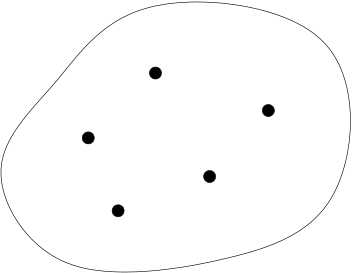
\includegraphics[width=2.2cm]{figures/example-set.png}}; \endxy}
  \qquad\qquad 
\begin{array}{c}
{\bf Categories} \\
  \text{isomorphisms $x \cong y$}
\end{array} \quad 
\xy (0,0)*{
 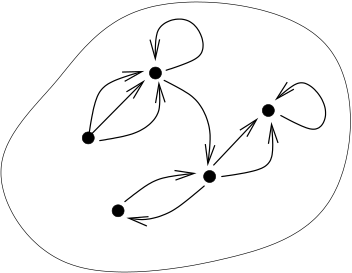
\includegraphics[width=2.2cm]{figures/example-cat.png}}; \endxy
\]
Equalities are lifted to explicit isomorphisms built from the new higher structure of categories.  The morphisms at the categorical level are a structure not seen at the `decategorified' or set level, but this new level of structure allows for far greater descriptive power.   This enhancement to categorical structures is where the term \emph{categorification} came from.   

After Crane and Frenkel's work, it became clear that categorification was prevalent throughout mathematics, with many well-known constructions naturally fitting into this framework, see ~\cite{Crane-Frenkel,Baez,KMS,LaudaSussan2022}.  Perhaps the best example to illustrate the key features of categorification might come from thinking about invariants of polyhedra.  It is well known that the Euler characteristic of the surface of a three-dimensional polyhedron is a topological invariant.  The quantity $\chi = (\#\text{vertices} - \#\text{edges}+\#\text{faces})$ remains the same for any polyhedron whose surface has the same underlying topology.  
\[
\xy
(0,0)*{
\begin{tikzpicture}
    \fill[gray!30] (0,0,0) -- (1,0,0) -- (1,1,0) -- (0,1,0) -- cycle;
    \fill[gray!30] (0,0,0) -- (0,0,1) -- (0,1,1) -- (0,1,0) -- cycle;
    \fill[gray!30] (0,0,0) -- (1,0,0) -- (1,0,1) -- (0,0,1) -- cycle;
    \fill[gray!30] (1,1,1) -- (0,1,1) -- (0,1,0) -- (1,1,0) -- cycle;
    \fill[gray!30] (1,1,1) -- (1,0,1) -- (1,0,0) -- (1,1,0) -- cycle;
    \fill[gray!30] (1,1,1) -- (1,0,1) -- (0,0,1) -- (0,1,1) -- cycle;
    \draw[dotted] (0,0,0) -- (1,0,0);
    \draw[dotted] (0,0,0) -- (0,0,1);
    \draw(1,0,0) -- (1,0,1);
    \draw[dotted] (0,1,0) -- (0,0,0);
    \draw (0,1,0) -- (0,1,1);
    \draw (1,0,1) -- (1,1,1);
    \draw (0,0,1) -- (1,0,1);
    \draw (0,0,1) -- (0,1,1);
    \draw (1,0,0) -- (1,1,0);
    \draw (1,1,0) -- (0,1,0);
    \draw (1,1,1) -- (1,1,0);
    \draw (1,1,1) -- (0,1,1);
    \foreach \x in {0,1}
        \foreach \y in {0,1}
            \foreach \z in {0,1}
                \fill[black] (\x,\y,\z) circle (2pt);
\end{tikzpicture}}; 
(0,-15)*{8-12+6=2};  
\endxy
\qquad  \qquad  \qquad 
\xy 
(0,0)*{
\begin{tikzpicture}[scale=1]
    \fill[gray!30] (1,1,0) -- (2,0,0) -- (0,0,0) -- cycle;
    \fill[gray!30] (1,1,0) -- (2,0,0) -- (1,0,2) -- cycle;
    \fill[gray!30] (1,1,0) -- (0,0,0) -- (1,0,2) -- cycle;
    \fill[gray!30] (0,0,0) -- (2,0,0) -- (1,0,2) -- cycle;
    \draw (1,1,0) -- (2,0,0);
    \draw[dotted] (2,0,0) -- (0,0,0);
    \draw (0,0,0) -- (1,1,0);
    \draw (1,1,0) -- (1,0,2);
    \draw (2,0,0) -- (1,0,2);
    \draw (0,0,0) -- (1,0,2); 
    \draw[dashed] (1,1,0) -- (1,0,2);
    \draw[dashed] (2,0,0) -- (1,0,2);
    \draw[dashed] (0,0,0) -- (1,0,2);
    \fill[black] (1,1,0) circle (2pt);
    \fill[black] (2,0,0) circle (2pt);
    \fill[black] (0,0,0) circle (2pt);
    \fill[black] (1,0,2) circle (2pt);
\end{tikzpicture} 
};
(0,-15)*{4-6+4=2};  
\endxy
\]
Later, of course, it was realized that there is a far more powerful set of invariants that not only apply to polyhedra but any sufficiently nice topological space $X$.  These are the (singular) homology groups, a collection of vector spaces\footnote{More generally abelian groups.} $H_i(X)$ associated to $X$.  We can forget information and simplify the vector spaces $H_i(X)$ into numerical quantities $\beta_i = \dim H_i(X)$ called the $i$-th Betti numbers.  The Euler characteristic is then the alternating sum of the Betti numbers.  

We say that homology groups categorify the Euler characteristic in that we have a well-defined procedure for forgetting information and producing a number.  The homology groups are a collection of vector spaces with the property that
\[
 \chi(X) = \sum_{i \geq 0} (-1)^i \dim H_i(X). 
\]
Finding a collection of vector spaces with this property on its own is not remarkable.  However, homology has a number of key advantages.  
\begin{itemize}
\item Homology is a more powerful invariant:  each $\beta_i$ is an invariant of $X$.  More spaces can be distinguished using homology than using Euler characteristic.    
\item Homology groups provide new insights into the meaning of the numeric quantities used to compute the Euler characteristic.  Betti numbers are dimensions of homology groups which themselves come from some topologically meaningful construction.  
\item Homology is functorial: given a continuous map $f:X\to Y$ between topological spaces, we get a map between the respective homologies $f_*:H_i(X)\to H_i(Y)$, compatible with composition and identity maps. This has important consequences for computing homology and provides an explanation for how continuous maps act on homology. This level could not have been seen if we had not lifted the Euler characteristic from a numerical invariant to the category of vector spaces and linear maps.
\end{itemize}

\begin{example}
The Euler characteristic of the 2-sphere $S^2$ is categorified by its homology groups $H_i(S^2)$:
\[
\xy
(0,0)*{
\begin{tikzpicture}[scale=.5]
\node at (.75,0) {$\begin{tikzpicture} [fill opacity=0.2, scale=.45]
	\path [fill=black] (0,0) circle (1);
	\draw (-1,0) .. controls (-1,-.4) and (1,-.4) .. (1,0);
	\draw[dashed] (-1,0) .. controls (-1,.4) and (1,.4) .. (1,0);
	\draw[very thick] (0,0) circle (1);
	\end{tikzpicture}$};
\draw[|->] (2,.5) to (4.7,1.5);
\draw[|->] (2,-.5) to (5,-1.5);
\draw[|->, very thick] (7,.7) to (7,-.7);
\node at (9.5,1.5) {$\mathrm{H}_{\bullet}\left(\sphere[.3];\mathbb C\right) \cong \mathbb C \oplus 0 \oplus \mathbb C$};
\node at (8,-1.5) {$\chi\left(\sphere[.3]\right)$ = 2};
\draw[thick, |->] (11,-1.5) to [out=20,in=-90] (12,1);
  \path [fill=white] (10.35,-.5) rectangle (13.65,.5);
\node at (12,0) {$\text{Categorification}$};
\end{tikzpicture}};
\endxy
\]
\[\chi(S^2) = \sum_{i=0}^{\infty} (-1)^i \dim H_i(S^2) = 1 - 0 +1 =2.\]
\end{example}
  


In this article, we will be interested in another kind of homology that categorifies the Jones polynomial in a similar sense. To motivate its construction, we start by considering the categorification of natural numbers. 
  
 
At the most primitive level, a natural categorification of the set $\Z_{\geq 0}$ is the category $\text{Vect}_\mathbb{C}$ of finite-dimensional vector spaces over  $\mathbb C$. A vector space $V$ is associated with its dimension $n = \operatorname{dim} V$, for which addition and multiplication on $\Z_{\geq 0}$ extend to $\text{Vect}_\mathbb{C}$ via the rules
\begin{equation}
 \operatorname{dim}(V \oplus W)=\operatorname{dim} V+\operatorname{dim} W, \qquad 
 \operatorname{dim}(V \otimes W)=\operatorname{dim} V \cdot \operatorname{dim} W.
\end{equation}
This means all the original structures of $\Z_{\geq 0}$ can be seen as decategorifications of operations on $\text{Vect}_\mathbb{C}$ that are simplified by applying the dimension map. 

At this point, it is again important to note that while any natural number $n$ can be categorified by $\mathbb{C}^n$, this would be an extremely naive categorification that would not by itself produce the desired properties we observe in the example of homology groups and the Euler characteristic.  Nevertheless, this is an excellent starting point for understanding the structure that would be needed to categorify the Jones polynomial.  


The Jones polynomial is not just a numerical invariant; it is a Laurent polynomial in $\mathbb{Z}[q,q^{-1}]$, which can be thought of as a sequence of numerical invariants corresponding to the coefficient of powers of $q$ appearing in $J(K)$. A Laurent polynomial $f \in$ $\mathbb{Z}_{\geq 0}\left[q, q^{-1}\right]$ with non-negative coefficients can be categorified by a $\mathbb{Z}$-graded vector space with decategorification corresponding to the \emph{graded} dimension $\operatorname{gdim} V$:
\begin{equation}
V=\bigoplus_{n \in \mathbb{Z}} V_n, \quad \operatorname{gdim} V:=\sum_{n \in \mathbb{Z}} q^n \operatorname{dim} V_n .
\end{equation}
In this context, the exponent of the variable $q$ encodes the grading on the vector space $V$. 
Hence, Laurent polynomials with non-negative coefficients are categorified by the category of finite-dimensional $\mathbb{Z}$-graded vector spaces, and decategorification is taking the graded dimension. 
 

The above constructions are not sufficient to categorify polynomials with negative coefficients, such as the Jones polynomial. To introduce the needed minus signs within a categorical setting,  it is natural to pass to chain complexes of graded vector spaces
\begin{equation}
V^{\cdot}=\cdots \longrightarrow V^i \xrightarrow{d} V^{i+1} \xrightarrow{d} V^{i+2} \longrightarrow \cdots ,
\end{equation}
consisting of a sequence of graded vector spaces $V^i$ and maps $d \maps V^i \to V^{i+1}$ satisfying $d^2=0$.   Such chain complexes give rise to homology groups as explained in \Cref{sec:chain}.  In this context, decategorification is given by taking  the \emph{graded Euler characteristic}
\begin{equation} \label{eq:gradedEuler}
    \chi\left(V^{\cdot}\right):=\sum_{i \in \mathbb{Z}}(-1)^i \operatorname{gdim} V^i  
\end{equation}
where the minus signs appear from odd homological degrees.   

Hence, to categorify the Jones polynomial, we need to construct a chain complex whose graded Euler characteristic recovers the Jones polynomial in such a way that the categorification has similar desired properties as the homology and Euler characteristic of topological spaces.  Naively taking $\mathbb{C}^n$'s with trivial differential would not by itself provide the desired cobordism maps or a proof of Reidemeister invariance for a diagrammatic construction.     For more on the interpretation of (graded) Euler characteristics in the broader context of decategorification, see \cite{Beliakova} and for a further introduction to categorification see \cite{LaudaSussan2022}.
 
\subsection{Khovanov homology}
\label{sec:khovanov_homology_background}
 
Khovanov homology \cite{Kh1} is a homology theory whose Euler characteristic is the Jones polynomial of a knot or link $K$. Each homology group $Kh^i(K)$ is a graded vector space $Kh^i(K)=\bigoplus_{j}Kh^{i,j}(K)$ and taking the graded Euler characteristic by the alternating sum of the graded dimensions of these groups, as in the previous section, gives the Jones polynomial,
\[
\mathrm{J}(K) = \sum_{i,j} (-1)^i q^j \dim( \mathrm{Kh}^{i,j}(K) ) .
\]
Each group $Kh^{i,j}(K)$ is a topological invariant of $K$.
\subsubsection{Why categorify?} \label{subsubsec-Why}
The power of Khovanov homology comes from the fact that it contains more information than the Jones polynomial.   Like the example of singular homology groups and Euler characteristics in the previous section, Khovanov homology has key advantages over the Jones polynomial.  

\begin{itemize}
    \item Khovanov homology groups $Kh^{i,j}(K)$ are strictly stronger knot invariants than $J(K)$.  Many knots with the same Jones polynomial have different Khovanov homologies~\cite{BN1}. 

\item Khovanov homology detects the unknot~\cite{KM}, trefoils~\cite{MR4393789}, the Hopf link~\cite{MR4049809}, and other specific knots~\cite{MR4275096}. Unlink detection is also known with appropriate coefficient and module information~\cite{Hedden}; that statement should not be conflated with the complex Betti numbers targeted here.
    
    \item Khovanov homology is functorial up to sign: functoriality in the context of knots and links requires a higher degree of topological sophistication. In this context, a map between two knots $K_1$ and $K_2$ is a smooth oriented surface $\Sigma$ properly embedded in $[0,1]\times\R^3$, with boundary the two knots in the endpoint slices. Such an embedded surface is called a \emph{knot cobordism}
    \[
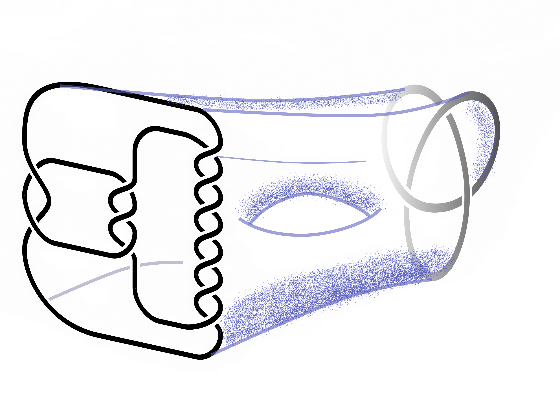
\includegraphics[width=2in]{figures/knot-cobordism.png}
\] 
    
    While it is difficult to draw meaningful illustrations\footnote{Thanks to Peter Kronheimer for the use of this knot cobordism illustration.},
    knot cobordisms belong to a part of knotted structures living in 4-dimensions. Khovanov homology is functorial in the sense that to any link cobordism $K_1 \xrightarrow{\Sigma} K_2$ it associates a map on homology, well defined up to an overall sign \cite{Jacobsson2004}. Sign-refined versions of the theory remove this ambiguity \cite{ClarkMorrisonWalker2009}.
\[
\xy
(0,0)*{
\begin{tikzpicture} [rotate=90, scale=.4]
\node at (0,5) {$
\xy
(0,0)*{
\begin{tikzpicture} [scale=.35]
\draw[very thick] (0,0) to [out=90,in=270] (.5,1);
\draw[very thick] (.2,.6) to [out=135,in=270] (0,1);
\draw[very thick] (.5,0) to [out=90,in=315] (.3,.4);
\draw[very thick] (0,-1) to [out=90,in=270] (.5,0);
\draw[very thick] (.2,-.4) to [out=135,in=270] (0,0);
\draw[very thick] (.5,-1) to [out=90,in=315] (.3,-.6);
\draw[very thick] (0,-2) to [out=90,in=270] (.5,-1);
\draw[very thick] (.2,-1.4) to [out=135,in=270] (0,-1);
\draw[very thick] (.5,-2) to [out=90,in=315] (.3,-1.6);
\draw[very thick, directed=.5] (.5,1) to [out=90,in=180] (.75,1.4) to [out=0,in=90] (1,1) to
	(1,-2) to [out=270,in=0] (.75,-2.4) to [out=180,in=270] (.5,-2);
\draw[very thick, directed=.5] (0,1) to [out=90,in=0] (-.25,1.4) to [out=180,in=90] (-.5,1) to
	(-.5,-2) to [out=270,in=180] (-.25,-2.4) to [out=0,in=270] (0,-2);
\end{tikzpicture}
}
\endxy
$};
\node at (0,0) {$
\xy
(0,0)*{
\begin{tikzpicture} [scale=.35]
\draw[very thick] (0,0) to [out=90,in=270] (.5,1);
\draw[very thick] (.2,.6) to [out=135,in=270] (0,1);
\draw[very thick] (.5,0) to [out=90,in=315] (.3,.4);
\draw[very thick] (0,-1) to [out=90,in=270] (.5,0);
\draw[very thick] (.2,-.4) to [out=135,in=270] (0,0);
\draw[very thick] (.5,-1) to [out=90,in=315] (.3,-.6);
\draw[very thick, directed=.5] (.5,1) to [out=90,in=180] (.75,1.4) to [out=0,in=90] (1,1) to
	(1,-1) to [out=270,in=0] (.75,-1.4) to [out=180,in=270] (.5,-1);
\draw[very thick, directed=.5] (0,1) to [out=90,in=0] (-.25,1.4) to [out=180,in=90] (-.5,1) to
	(-.5,-1) to [out=270,in=180] (-.25,-1.4) to [out=0,in=270] (0,-1);
\end{tikzpicture}
}
\endxy
$};
	\draw[thick] (-1.5,4.375) to [out=225,in=90] (-1.25,2.5) to [out=270,in=135] (-1.25,.625);
	\draw[thick] (1.5,4.375) to [out=315,in=90] (1.25,2.5) to [out=270,in=45] (1.25,.625);
	\fill[red,opacity=.2] (-1.5,4.375) to [out=225,in=90] (-1.25,2.5) to [out=270,in=135] (-1.25,.625) to
		(1.25,.625) to [out=45,in=270] (1.25,2.5) to [out=90,in=315] (1.5,4.375);
	\fill[white] (0,3) to [out=300,in=60] (0,2) to [out=120,in=240] (0,3);
	\draw[thick] (0,3) to [out=300,in=60] (0,2);
	\draw[thick] (0.1,1.8) to [out=125,in=235] (0.1,3.2);
\end{tikzpicture}
};
\endxy
\quad
\leadsto
\quad
\mathrm{Kh}\left( \;
\xy
(0,0)*{
\begin{tikzpicture} [scale=.35]
\draw[very thick] (0,0) to [out=90,in=270] (.5,1);
\draw[very thick] (.2,.6) to [out=135,in=270] (0,1);
\draw[very thick] (.5,0) to [out=90,in=315] (.3,.4);
\draw[very thick] (0,-1) to [out=90,in=270] (.5,0);
\draw[very thick] (.2,-.4) to [out=135,in=270] (0,0);
\draw[very thick] (.5,-1) to [out=90,in=315] (.3,-.6);
\draw[very thick] (0,-2) to [out=90,in=270] (.5,-1);
\draw[very thick] (.2,-1.4) to [out=135,in=270] (0,-1);
\draw[very thick] (.5,-2) to [out=90,in=315] (.3,-1.6);
\draw[very thick, directed=.5] (.5,1) to [out=90,in=180] (.75,1.4) to [out=0,in=90] (1,1) to
	(1,-2) to [out=270,in=0] (.75,-2.4) to [out=180,in=270] (.5,-2);
\draw[very thick, directed=.5] (0,1) to [out=90,in=0] (-.25,1.4) to [out=180,in=90] (-.5,1) to
	(-.5,-2) to [out=270,in=180] (-.25,-2.4) to [out=0,in=270] (0,-2);
\end{tikzpicture}
}
\endxy
\; \right)
\xrightarrow{\mathrm{Kh}(\Sigma)}
\mathrm{Kh}\left( \;
\xy
(0,0)*{
\begin{tikzpicture} [scale=.35]
\draw[very thick] (0,0) to [out=90,in=270] (.5,1);
\draw[very thick] (.2,.6) to [out=135,in=270] (0,1);
\draw[very thick] (.5,0) to [out=90,in=315] (.3,.4);
\draw[very thick] (0,-1) to [out=90,in=270] (.5,0);
\draw[very thick] (.2,-.4) to [out=135,in=270] (0,0);
\draw[very thick] (.5,-1) to [out=90,in=315] (.3,-.6);
\draw[very thick, directed=.5] (.5,1) to [out=90,in=180] (.75,1.4) to [out=0,in=90] (1,1) to
	(1,-1) to [out=270,in=0] (.75,-1.4) to [out=180,in=270] (.5,-1);
\draw[very thick, directed=.5] (0,1) to [out=90,in=0] (-.25,1.4) to [out=180,in=90] (-.5,1) to
	(-.5,-1) to [out=270,in=180] (-.25,-1.4) to [out=0,in=270] (0,-1);
\end{tikzpicture}
}
\endxy
\; \right)
\]
\end{itemize}

\begin{remark}
The functoriality of Khovanov homology encodes deep structures that can probe the smooth topology of 4-manifolds~\cite{Rasmussen}.  These structures have been used to prove results previously only accessible using gauge theory~\cite{Rasmussen}, as well as provide new constructions of exotic smooth 4-manifolds~\cite{Ren-WIllis}.  
\end{remark}

 


\subsubsection{Lifting the Kauffman bracket} \label{subsec:lifting-Kauffman}

We now describe the construction of Khovanov homology given a planar representation of a knot $K$.  We first lift the Kauffman bracket $\langle K \rangle$ to the \emph{Khovanov bracket}  $\llangle K  \rrangle$.  The Khovanov bracket is a chain complex whose homology is the Khovanov homology up to some overall shifts explained in \Cref{subsec:Kh-bracket-homology}.  For more details see ~\cite{Kh1,BN1}.

Fix an ordering of the $m$ crossings in the knot diagram for $K$.  
By choosing at each of the $m$ crossings of $K$ either a 0-smoothing $\langle\KPC\rangle$ or 1-smoothing $\langle\KPD\rangle$ (cf. \Cref{sec:Jones_polynomial}), we arrive at a crossingless diagram which we call a resolution (or state), denoted by an $m$-bit string $r$ whose $j$-th bit specifies which smoothing was applied to the crossing labeled $j$.  The Hamming weight of the state $\ket{r}$ is denoted $|r|$ and equals the number of 1-smoothings in the resolution.

Each resolution ${r}$ is associated with a number $\ell(r)$ of disjoint loops resulting from the resolution, see the right-hand side of Figure~\ref{fig:Kauffman1}. In this notation, the Kauffman bracket can be written in its ``state sum'' representation 
\begin{equation} \label{eq:Kauff}
    \langle K \rangle = \sum_{r\in \{0,1\}^m}(-q)^{|r|}(q+q^{-1})^{\ell(r)}.
\end{equation}
It is easy to verify that this expression agrees with the recursive definition in \Cref{sec:Jones_polynomial}.

The central idea of Khovanov homology is to take the alternating sum in \cref{eq:Kauff} and interpret it as an Euler characteristic of some homology theory.  To account for the $q$ factors that appear, our homology theory will carry an additional grading as in \cref{eq:gradedEuler}, and the Kauffman bracket will be categorified by a graded homology theory whose graded Euler characteristic recovers the Kauffman bracket. 
 
Since a loop gets replaced by $(q+q^{-1})$ in the Kauffman bracket,  to construct the Khovanov bracket $\llangle K \rrangle$ this Laurent polynomial associated with a loop is categorified to a graded vector space $V=\mathbb{C}_{-1} \oplus \mathbb{C}_{+1}$ that is one-dimensional in degrees $\pm 1$ and zero in all other degrees, so that $\operatorname{gdim}V = (q+q^{-1})$.  We fix a graded basis for $V$ that we denote by  $\1$ and $X$, with $\deg(\1)=1$ and $\deg(X)=-1$ following the conventions from \cite{Kh1}
and think of these as labels on the loop.  

More generally, we can categorify all of the terms in \cref{eq:Kauff}.  The space $V^{\otimes \ell(r)}$ will have graded dimension $(q+q^{-1})^{\ell(r)}$.   Define the $i$th chain space $\llangle K\rrangle^i$ of the Khovanov bracket $\llangle K\rrangle$ chain complex    by setting 
\begin{equation} \label{eq:Kh-C}
    \llangle K\rrangle^i = \bigoplus_{ |r|=i} V^{\otimes \ell(r)} \langle i \rangle,
\end{equation}
where $\langle i \rangle$ is the grading shift operation that shifts the overall grading by $i$ such that
\begin{equation}
 \operatorname{gdim} V \langle i \rangle = q^i  \operatorname{gdim} V.
\end{equation}
The number $i$ is called the \emph{(co)homological degree} and counts how many $1$-smoothings appear in the resolution. Observe that with this grading shift, $\operatorname{gdim} \llangle K\rrangle^i = \sum_{|r|=i} q^{i}(q+q^{-1})^{\ell(r)}$. 


Choosing a basis vector for each of the $\ell(r)$ loops appearing in a resolution $r$ of the knot $K$ assigns a label that is either $\1$ or $X$. The possible labeling of the loops are thus described by a $\ell(r)$-bit string $s$, where a 0 encodes the state $\1$, and a 1 encodes the state $X$. The tuples $(r,s)$ that specify both the choice of smoothings and the labels of the resulting loops are called \emph{enhanced states}.  
The Hamming weight $|s|$ denotes the number of loops in the state $X$, while $\ell(r)-|s|$ is the number of loops in state $\1$.    

Each enhanced state $(r,s)$ carries two gradings, the \emph{homological degree} $i:= |r|$ given by the number of 1-resolutions in $r$, and the \emph{quantum grading} $j$ associated with the labels in the enhanced state $s$.  The quantum grading is defined as $j= i  + \ell(r)-2|s|$, which comes from the overall shift by $i$, plus the number of loops labeled $\1$, and minus the number of loops labeled $X$.  Hence, each $\llangle K\rrangle^i$ further splits into $\llangle K\rrangle^i=\bigoplus_{j}\llangle K\rrangle^{i,j}$. 
 
The graded Euler characteristic is the alternating sum of the dimensions of the homology groups, but if the differential preserves the grading and all the chain groups are finite dimensional then one can show that the Euler characteristic is also the alternating sum of the graded dimensions of the chain spaces,
\[
 \chi(\llangle K\rrangle) = \sum_{i} (-1)^i {\rm gdim} H^i(\llangle K\rrangle) = \sum_i (-1)^i {\rm gdim} (\llangle K\rrangle^i), 
\] which now matches \cref{eq:Kauff}.
Hence, we could build a naive categorification of the  Kauffman bracket from our complex $\llangle K\rrangle$ with chain spaces as in \cref{eq:Kh-C} and trivial differentials.  
\[
 \chi(\llangle K\rrangle) 
 = \sum_i (-1)^i {\rm gdim} (\llangle K\rrangle^i) 
  = \sum_{i,j} (-1)^i q^j{\rm  dim} (\llangle K\rrangle^{i,j}) 
 = \langle K \rangle.
\]
However, this naive categorification is not invariant under Reidemeister moves. Its graded chain dimensions may contain more information than the Kauffman bracket, but a suitable differential is needed to obtain the homological link invariant described in \Cref{subsubsec-Why}.


\subsubsection{Khovanov boundary operator} \label{subsec:Kh-boundary-intro}

The nontrivial content of Khovanov homology is specified by the differential on the complex $\llangle K\rrangle$   associated to a knot. To specify the differential in Khovanov homology, we make use of the following maps on the vector space $V=\langle \1, X\rangle$ associated with loops in a resolution
\begin{alignat}{3} \label{eq:mdelta}
 m\maps V\otimes V&\to V   \qquad \qquad    && \delta \maps V \to V\otimes V 
 \\   \nonumber
 \ket{\1\1} &\mapsto \ket{\1} \qquad \qquad    && \quad\; \ket{\1} \mapsto \ket{\1X} + \ket{X\1}  
 \\ \nonumber
 \ket{\1X} &\mapsto \ket{X} \qquad \qquad    && \quad\; \ket{X} \mapsto \ket{XX}  
 \\ \nonumber
\ket{X\1}  &\mapsto \ket{X} 
\\ \nonumber
\ket{XX}  &\mapsto 0  \nonumber
\end{alignat}
With the gradings given by $\deg(\1)=1$ and $\deg(X)=-1$, one can check that both maps have degree -1, meaning they decrease the grading by one.  If we add an additional grading shift of $\langle1\rangle$ on the targets so that $m \maps V\otimes V \to V\langle1\rangle$ and $\delta\maps V \to V \otimes V\langle1\rangle$, then these maps will have degree zero, meaning they preserve the quantum degree $j$.
  

The differential $d \maps C^i \to C^{i+1}$ in the Khovanov bracket $\llangle K\rrangle$
decomposes as a sum of maps $d_{r,v}$ over pairs $(r,v)$ consisting of a resolution $r$ with $|r|=i$ and a resolution $v$  obtained from $r$ by swapping a single $0$ to a $1$ in $r$.  The number of loops in the resolutions for such pairs of $r$ and $v$ will always have $|\ell(r)-\ell(v)|=1$, and the map $d_{r,v}$ can be thought of as either merging two loops into one or splitting one loop into two.  See Figure~\ref{fig:Kh-Hopf} for a simple example.

\begin{figure}
    \centering
$
\begin{tikzpicture}
 \node (T) at (-4,1.65) {  $\left\llangle \; \hackcenter{
    \begin{tikzpicture}[scale=.4]
  \draw [black, very thick]    (2,1) .. controls +(0,.25) and +(0,-.25) .. (1,2);
  \draw [black, very thick]    (2,2) .. controls +(0,.25) and +(0,-.25) .. (1,3);
  \path [fill=white] (1.35,1) rectangle (1.65,3);
  \draw [black, very thick]    (1,1) .. controls +(0,.25) and +(0,-.25) .. (2,2);
  \draw [black, very thick]    (1,2) .. controls +(0,.25) and +(0,-.25) .. (2,3);
  \draw [black, very thick]    (1,3) .. controls +(-.1,.5) and +(+.1,.5) .. (0,3);
  \draw [black, very thick]    (2,3) .. controls +(+.1,.5) and +(-.1,.5) .. (3,3);
  \draw [black, very thick]    (0,3) -- (0,1);
  \draw [black, very thick]    (3,3) -- (3,1);
  \draw [black, very thick]    (1,1) .. controls +(-0.1,-0.5) and+(+0.1,-0.5) .. (0,1);
  \draw [black, very thick]    (2,1) .. controls +(0.1,-0.5) and +(-0.1,-0.5) .. (3,1);
    \end{tikzpicture} } \; \right\rrangle$  };
 \node (B4) at (3,0) {
        \begin{tikzpicture}[scale=.4]
  \draw [black, very thick]    (1,1) .. controls +(0,.35) and +(0,.35) .. (2,1);
  \draw [black, very thick]    (2,2) .. controls +(0,-.35) and +(0,-.35) .. (1,2);
  \draw [black, very thick]    (1,2) .. controls +(0,.35) and +(0,.35) .. (2,2);
  \draw [black, very thick]    (2,3) .. controls +(0,-.35) and +(0,-.35) .. (1,3);
  \draw [black, very thick]    (1,3) .. controls +(-.1,.5) and +(+.1,.5) .. (0,3);
  \draw [black, very thick]    (2,3) .. controls +(+.1,.5) and +(-.1,.5) .. (3,3);
  \draw [black, very thick]    (0,3) -- (0,1);
  \draw [black, very thick]    (3,3) -- (3,1);
  \draw [black, very thick]    (1,1) .. controls +(-0.1,-0.5) and+(+0.1,-0.5) .. (0,1);
  \draw [black, very thick]    (2,1) .. controls +(0.1,-0.5) and +(-0.1,-0.5) .. (3,1);
    \end{tikzpicture}};
 \node (B3) at (0,-1.5) {
        \begin{tikzpicture}[scale=.4]
  \draw [black, very thick]    (1,2) -- (1,1);
  \draw [black, very thick]    (2,2) -- (2,1);
  \draw [black, very thick]    (1,2) .. controls +(0,.35) and +(0,.35) .. (2,2);
  \draw [black, very thick]    (2,3) .. controls +(0,-.35) and +(0,-.35) .. (1,3);
  \draw [black, very thick]    (1,3) .. controls +(-.1,.5) and +(+.1,.5) .. (0,3);
  \draw [black, very thick]    (2,3) .. controls +(+.1,.5) and +(-.1,.5) .. (3,3);
  \draw [black, very thick]    (0,3) -- (0,1);
  \draw [black, very thick]    (3,3) -- (3,1);
  \draw [black, very thick]    (1,1) .. controls +(-0.1,-0.5) and+(+0.1,-0.5) .. (0,1);
  \draw [black, very thick]    (2,1) .. controls +(0.1,-0.5) and +(-0.1,-0.5) .. (3,1);
        \end{tikzpicture}};
 \node (B2) at (0,1.5) {
        \begin{tikzpicture}[scale=.4]
  \draw [black, very thick]    (1,1) .. controls +(0,.35) and +(0,.35) .. (2,1);
  \draw [black, very thick]    (2,2) .. controls +(0,-.35) and +(0,-.35) .. (1,2);
  \draw [black, very thick]    (1,2) -- (1,3);
  \draw [black, very thick]    (2,2) -- (2,3);
  \draw [black, very thick]    (1,3) .. controls +(-.1,.5) and +(+.1,.5) .. (0,3);
  \draw [black, very thick]    (2,3) .. controls +(+.1,.5) and +(-.1,.5) .. (3,3);
  \draw [black, very thick]    (0,3) -- (0,1);
  \draw [black, very thick]    (3,3) -- (3,1);
  \draw [black, very thick]    (1,1) .. controls +(-0.1,-0.5) and+(+0.1,-0.5) .. (0,1);
  \draw [black, very thick]    (2,1) .. controls +(0.1,-0.5) and +(-0.1,-0.5) .. (3,1);
    \end{tikzpicture}};
  \node (B1) at (-3,0) {\begin{tikzpicture}[scale=.4]
  \draw [black, very thick]    (1,1) -- (1,3);
  \draw [black, very thick]    (2,1) -- (2,3);
  \draw [black, very thick]    (1,3) .. controls +(-.1,.5) and +(+.1,.5) .. (0,3);
  \draw [black, very thick]    (2,3) .. controls +(+.1,.5) and +(-.1,.5) .. (3,3);
  \draw [black, very thick]    (0,3) -- (0,1);
  \draw [black, very thick]    (3,3) -- (3,1);
  \draw [black, very thick]    (1,1) .. controls +(-0.1,-0.5) and+(+0.1,-0.5) .. (0,1);
  \draw [black, very thick]    (2,1) .. controls +(0.1,-0.5) and +(-0.1,-0.5) .. (3,1);
    \end{tikzpicture}};
  \draw [thick,->] (B1) -- (B2);
  \draw [thick,->] (B1) -- (B3);
  \draw [thick,->] (B2) -- (B4);
  \draw [thick,->] (B3) -- (B4);
 \node at (-3,-1) {$\ket{00}$ };
 \node at (0,-2.5) {$\ket{10}$ };
\node at (0,.5) {$\ket{01}$ };
 \node at (3,-1) {$\ket{11}$ };
  \node at (-1.5,-1.25) {$m$};
  \node at (-1.5,1.25) {$m$};
 \node at (1.5,-1.25) {$-\delta$};
 \node at (1.5,1.25) {$\delta$};
\end{tikzpicture}
$
    \caption{\justifying An illustration of the Khovanov complex associated with the Hopf link.  Each resolution is arranged in a column by Hamming weight.  The differential connects edges related by swapping a single 0 to a 1 and has the effect of merging or splitting two circles.  Each merge of two circles is associated with the map $m$, and each split is associated with the map $\delta$.  }
    \label{fig:Kh-Hopf} 
\end{figure}

If $r=r_1 \dots r_{a-1}0r_{a+1} \dots r_m$ and $v = v_1 \dots v_{a-1} 1 v_{a+1} \dots v_m$, then
\begin{equation} \label{eq:Kh-d}
    d^i = \sum_{r,v :  |r|=i} (-1)^{v_1 + \dots + v_{a-1}} d_{r,v},
\end{equation}
where $d_{r,v}$ acts trivially on all copies of $V$ not involved in the split or merge and 
\begin{itemize}
    \item if $d_{r,v}$ merges two loops into one, then $d_{r,v}$ applies the map $m\maps V \otimes V \to V$ on the copies of V associated with the loops being merged, and 
    \item if $d_{r,v}$ splits one loop into two, then $d_{r,v}$ acts by the map $\delta\maps V \to V \otimes V$ on the loop being split into two. 
\end{itemize}
Note that the grading shift of $\langle i \rangle$ on $\llangle K\rrangle^i$ and $\langle i +1\rangle$ on $\llangle K\rrangle^{i+1}$ from \cref{eq:Kh-C} ensures that these differentials are (quantum) degree preserving.  
One can check that with this definition $d^{i+1}\circ d^i = 0$.   This differential on $\llangle K\rrangle$ gives rise to the highly nontrivial nature of Khovanov's categorification of the Jones polynomial. 


In Section~\ref{subsec:Kh-boundary} we give a quantum interpretation of the Khovanov differential, where the signs in \cref{eq:Kh-d} have a natural interpretation via Jordan Wigner creation operators.  


\subsubsection{From the Khovanov bracket to Khovanov homology} \label{subsec:Kh-bracket-homology}

Just as the Jones polynomial is obtained from the Kauffman bracket via an overall rescaling by $(-1)^{n_-} q^{n_+ -2n_-}$ as in \cref{eq:Jones-shift} to fix Reidemeister  invariance, the complex $\mathbf{C}$ used to compute Khovanov homology is obtained by an overall shift  in homological degree by $-n_-$ and quantum degree shift by $\langle n_+ -2n_-\rangle$, so that $\mathbf{C}(K)= \llangle K \rrangle [-n_-]\langle n_+ -2n_-\rangle$ meaning that the bigraded chain spaces in Khovanov homology are given by
\[
C(K)^{i,j}  : = \llangle K \rrangle^{i+n_-, j-n_+ +2n_-}.
\]
Here $[s]$ is the homological height shift operation that shifts the index of a complex $\mathbf{C}$ so that $C[s]^i := C^{i-s}$ with the differentials shifted accordingly.  

With these new shifts, we have the following:
\begin{theorem}[\cite{Kh1}]
    The graded Euler characteristic of $\mathbf{C}(K)$ is the Jones polynomial of $K$ in the normalization of \cref{eq:Jones-shift}, for which $J(\KPA)=q+q^{-1}$.
    \[
\chi ( \mathbf{C}(K) ) = J(K).
\]
\end{theorem}

The Khovanov homology of a knot $K$ is the homology of the complex $\mathbf{C}(K)$.  
Let $H^i(\mathbf{C}(K))$ be the $i$th homology of the complex $\mathbf{C}(K)$.  Since all the differentials in this complex have (quantum) degree zero, the homology splits as a direct sum of quantum degrees 
\[
H^i(\mathbf{C}(K))= \bigoplus_j H^{i,j}\mathbf{C}(K),
\]
and we define  $Kh^{i,j}(K):= H^{i,j}(\mathbf{C}(K))$.   Our goal in this article is to compute the graded Betti numbers $\beta_{i,j}(K):= \dim Kh^{i,j}(K)$.

\medskip
\noindent \textbf{Reduced Khovanov homology.}  We will also use the reduced version of the theory \cite{KhovanovPatterns}, which is the version computed by the spanning-tree model of \Cref{sec:spanning_trees}.  Fix a basepoint on the diagram away from the crossings.  In every resolution the basepoint lies on exactly one loop, and the enhanced states in which this marked loop is labeled $X$ span a subcomplex of $\mathbf{C}(K)$, because the maps $m$ and $\delta$ of \cref{eq:mdelta} never replace an $X$ on the marked loop by $\1$.  This subcomplex, with the gradings inherited from $\mathbf{C}(K)$, is the \emph{reduced Khovanov complex} $\widetilde{\mathbf{C}}(K)$; its homology $\widetilde{Kh}^{i,j}(K)$ is the reduced Khovanov homology, and we write $\widetilde\beta_{i,j}(K):=\dim\widetilde{Kh}^{i,j}(K)$.  For a knot it is an invariant of $K$; for a link we retain the marked component as part of the input \cite{KhovanovPatterns,ChampanerkarKofmanMutation2008}.  With this grading the reduced homology of the unknot is $\mathbb{C}$ in bidegree $(0,-1)$ and $\chi(\widetilde{\mathbf{C}}(K))=J(K)/(q^2+1)=(-1)^{\ell(K)-1}q^{-1}V_K(q^2)$; this is the convention of \cite{champanerkar2008spanningtrees}, whose spanning-tree gradings we use in \Cref{sec:spanning_trees}, while many authors raise the quantum grading by one so that the reduced unknot sits in bidegree $(0,0)$.  The reduced and unreduced theories are related by the long exact sequence of the pair $(\mathbf{C}(K),\widetilde{\mathbf{C}}(K))$, and their total ranks differ in general. For the trefoil the unreduced homology has total rank $4$ and the reduced homology has total rank $3$.  The quantum protocol of \Cref{sec:kh_quantum_algorithm} targets the unreduced numbers $\beta_{i,j}$, while the classical benchmark of \Cref{sec:spanning_trees} concerns the reduced numbers $\widetilde\beta_{i,j}$.

For the purposes of this article, computing the homology of the Khovanov bracket $\llangle K\rrangle$ has the same difficulty as computing Khovanov homology since the two only differ by overall homological and quantum degree shifts. We retain these shifts in all invariant bidegrees, target-register predicates, and Jones-polynomial reductions below; an unshifted cube grading is explicitly identified when used.


\subsection{Unknot recognition}
\label{sec:intro_unknot}
An additional motivation for studying Khovanov homology arises from the \emph{unknot-recognition problem:}
\begin{quote}
    Given a knot diagram $D$, determine whether $D$ represents the unknot (the trivial knot with no crossings).
\end{quote}
The Jones polynomial of the unknot is $J(\KPA) = q+q^{-1}$, equivalently $V_{\KPA}(t)=1$ in the normalization of \cref{eq:Jones-normalized}. It is not known whether the Jones polynomial is a strong enough invariant to recognize the unknot, that is, whether the trivial knot is the only knot with this Jones polynomial. 

On the other hand, Khovanov homology is known to detect the unknot due to the seminal result by Kronheimer and Mrowka~\cite{KM}.  Kronheimer and Mrowka show that a knot $K$ is the unknot if and only if its Khovanov homology has the form
\begin{equation}
Kh^{i,j}(K) = \begin{cases} 
\mathbb{C} & \text{if } (i,j) = (0,1) \text{ or } (0,-1), \\
0 & \text{otherwise}. 
\end{cases}
\end{equation}
This means that any algorithm that can certify that the only nonzero Betti numbers of a knot are $\beta_{0,1}(K) = \beta_{0,-1}(K) = 1$ detects the unknot. 

It is a major unresolved challenge to determine whether there exists an efficient (polynomial time) algorithm for the unknot-recognition problem. After Haken \cite{haken1961theorie} showed in 1961 that knot-triviality is decidable, a sequence of works established increasingly tight upper bounds on the complexity class of the unknot-recognition problem. For a definition of these complexity classes, see \Cref{sec:complex_prelim}. Hass et al. \cite{HLP} showed in 1999 that the unknot-recognition problem is contained in $\NP$. Kuperberg \cite{kuperberg2014knottedness} showed that the unknot-recognition problem is also contained in $\mathsf{co}$-$\NP$, provided the generalized Riemann hypothesis holds. Lackenby \cite{lackenby2021efficient} later removed this hypothesis, giving an unconditional proof of $\mathsf{co}$-$\NP$ containment. This places the unknot-recognition problem in the complexity class $\NP$ $\cap$ $\mathsf{co}$-$\NP$.  Problems in this class cannot be $\NP$-complete unless $\NP=\mathsf{co}$-$\NP$, while membership in $\mathsf{P}$ remains open, so the unknot-recognition problem is a candidate \emph{$\NP$-intermediate} problem, in the same sense as integer factoring. An efficient quantum algorithm for such a problem does not clash with the widely held belief that $\NP \not \subseteq \BQP$. A well-studied candidate NP-intermediate problem is the factoring problem, which is famously solved efficiently on a quantum computer via Shor's algorithm. 

The unknot-recognition problem is only one motivation for studying Khovanov homology computationally.  The algorithmic framework below targets the Betti numbers themselves, and uses the Hodge-theoretic description of homology as the kernel of a Laplacian.
% ===================== END background.tex =====================


% ==================== BEGIN general-homology.tex ====================
\section{Quantum algorithms for general homology theories}\label{sec:general_homology}
The preceding section described the Khovanov complex as a finite-dimensional chain complex. We now recall the general Hodge-Laplacian method that turns such a complex into a quantum Hamiltonian problem. Quantum algorithms for computing the ranks of homology groups were first developed in \cite{lloyd2016quantum} in the context of clique homology and topological data analysis. Since then, these quantum algorithms have seen extensive follow-up work, see e.g. \cite{quantumAdvantage,persistent,IBMresult,GoogleBettiBerry,AmazonBettiMcArdle,schmidhuber2023complexity,crichigno2022clique,king2023gapped,hayakawa2024quantum,gyurik_schmidhuber_2024quantum}. Some of these works have considered extending the techniques to homologies that are more general than simplicial. Cade and Crichigno \cite{cade2021complexity} formally discussed sufficient requirements for efficiently estimating so-called \emph{normalized quasi-Betti numbers} on general complexes with log-local or sparse boundary operators.

A homology theory is specified by a chain complex \(C\), which is a sequence of abelian groups or vector spaces connected by homomorphisms whose successive compositions vanish. In anticipation of representing such a chain space on a quantum mechanical Hilbert space made out of qubits, we consider the case where \(C\) consists of finitely many chain spaces, each being a finite-dimensional vector space over the complex numbers \(\mathbb C\). We use the increasing cohomological grading of the Khovanov complex. Thus the boundary maps are \(\partial_i:C^i\to C^{i+1}\), with \(\partial_{i+1}\partial_i=0\), and the homology groups are \(H^i(C)=\ker\partial_i/\operatorname{im}\partial_{i-1}\).

Throughout the paper we use a Hodge-theoretic model of homology, which is more natural from the perspective of quantum computation. Fix inner products on the chain groups \(C^i\), and let \(\partial_i^\dagger\) denote the adjoint of the boundary map \(\partial_i\). The \(i\)-th Hodge Laplacian is
\[
 \Delta_i=\partial_i^\dagger\partial_i+
            \partial_{i-1}\partial_{i-1}^\dagger.
\]
Both summands are nonnegative Hermitian operators. For every \(x\in C^i\),
\[
 \langle x,\Delta_i x\rangle
 =\|\partial_i x\|^2+\|\partial_{i-1}^\dagger x\|^2.
\]
Hence any chain annihilated by \(\Delta_i\) lies in the intersection of the kernels of \(\partial_i\) and \(\partial_{i-1}^\dagger\). The first condition says that the chain is a cycle. The second says that it is orthogonal to \(\operatorname{im}\partial_{i-1}\), the subspace of boundaries in degree \(i\). Together these conditions select the harmonic representative of the homology class. In the finite-dimensional setting used here, the Hodge decomposition gives an orthogonal direct sum whose middle summand is naturally identified with homology,
\[
 C^i=\operatorname{im}\partial_{i-1}\oplus
       \ker\Delta_i\oplus\operatorname{im}\partial_i^\dagger,
 \qquad H^i(C)\cong\ker\Delta_i.
\]
We call \(\ker\Delta_i\) the harmonic subspace in degree \(i\). Thus every homology class has a unique \emph{harmonic representative}, namely its unique representative in \(\ker\Delta_i\). This representative depends on the chosen inner products. The dimension \(\beta_i\) of the kernel is invariant under chain homotopy equivalence, but its embedding and the nonzero eigenvalues of the Laplacian need not be.

The Laplacian \(\Delta_i\) is a self-adjoint linear operator acting on the complex vector space \(C^i\), and can therefore be interpreted as the Hamiltonian of a quantum mechanical system. Estimating the Betti number \(\beta_i=\dim H^i(C)=\dim\ker\Delta_i\) then corresponds to estimating the dimension of its zero-energy space, which is the ground-state space when \(\beta_i>0\). Finding the ground state of a quantum mechanical system is a canonical problem in quantum information theory, but cannot be assumed to be efficient for a general sparse Hamiltonian. The ground-energy problem is itself a source of quantum complexity-theoretic hardness \cite{kitaev2002classical,bookatz2012qma}.

With a slight abuse of notation, the chain complex is compactly specified by the graded vector space \(C=\bigoplus_iC^i\) and the boundary operator \(\partial\). The Hermitian operator \(B=\partial+\partial^\dagger\) on \(\bigoplus_iC^i\) obeys \(B^2=\Delta\). It mixes neighboring degrees; its square preserves each degree. If \(P_i\) is the projector onto \(C^i\), then \(P_iBP_i=0\), so the square of this restricted operator does not recover \(\Delta_i\) when that block is nonzero.

In the filtering-and-purity approach, the following requirements enter the runtime.
\begin{enumerate}
    \item The Hilbert space \(C\) has to have an efficient description. For example, it could be the subspace of a full \(n\)-qubit Hilbert space described by a polynomial number of efficiently checkable constraints. The boundary operator also needs an implementable sparse or log-local description. Efficient membership in a valid sector alone does not provide uniform sampling from that sector.
    \item State preparation has to give inverse-polynomial weight on the zero-energy space of the Laplacian. For Betti-number estimation by kernel-state purity, the preparation also has to be calibrated on the kernel, as in the Gibbs-state protocol discussed in \Cref{sec:thermalization}. The cost and accuracy of this preparation have to be included.
    \item The Hodge Laplacian has to have a normalized spectral gap at least inverse polynomial in the input size. Phase estimation must resolve zero from the first nonzero eigenvalue at the normalization used to implement the Hamiltonian, rather than at the unscaled gap alone.
\end{enumerate}
These requirements do not by themselves give an efficient rank estimate. The desired accuracy and the rank dependence of the measurement also contribute to the runtime, as quantified in \Cref{subsec:Kh-performance}.

The state-preparation requirement is the main departure from the original quantum homology algorithm. To describe it, let \(\Pi_i^0\) project onto \(\ker\Delta_i\). For a normalized density operator \(\rho\), put
\[
 w_i(\rho)=\operatorname{Tr}(\Pi_i^0\rho),\qquad
 \rho_{0,i}=\Pi_i^0\rho\Pi_i^0/w_i(\rho)
 \quad\text{if }w_i(\rho)>0.
\]
The first quantity is the success probability of an ideal zero-energy filter. We call \(\rho\) \emph{kernel-calibrated} if \(\rho_{0,i}=\Pi_i^0/\beta_i\). High overlap alone does not imply calibration. A pure harmonic vector has overlap one but gives no information about how many orthogonal harmonic vectors exist. Approximate calibration requires an explicit error tolerance. We use \(\|\cdot\|_1\) for the trace norm, so the conventional trace distance is half that norm.

The original algorithm prepares a uniform mixture on an orthonormal basis of \(C^i\),
\[
 \rho_{\rm unif}=I_{C^i}/\dim C^i,
 \qquad w_i(\rho_{\rm unif})=\beta_i/\dim C^i.
\]
It then uses quantum phase estimation to project onto \(\ker\Delta_i\). The success probability is \(\beta_i/\dim C^i\). Obtaining a harmonic state this way is effective only when the Betti number is not too small compared with the chain-space dimension. Given efficient preparation and a resolvable normalized spectral gap, repeated zero-energy tests also estimate this \emph{normalized} Betti number to additive accuracy. A small kernel probability is an obstacle to obtaining harmonic states by rejection, or to relative and exact estimation; it does not prevent a coarse additive estimate of a probability close to zero. Multiplying that estimate by an exponentially large chain dimension does not give an accurate unnormalized rank.

For Khovanov homology this ratio \(\beta_i/\dim C^i\) can be very small. We therefore investigate two complementary ideas. First, a topologically structured guiding state can improve the initial QPE overlap. The spanning-tree construction in \Cref{sec:spanning_trees} is one such source of guiding states. Direct QPE from that state is governed by its geometric overlap with the harmonic subspace, which is defined explicitly there. Second, for calibrated Betti-number estimation, we consider a low-temperature Gibbs state of the Hodge Laplacian, or another preparation whose projection to the kernel is close to maximally mixed. A Gibbs state \(e^{-\gamma H}/\operatorname{Tr}(e^{-\gamma H})\) is scalar on each eigenspace and thus exactly calibrated on a nonempty kernel. The Gibbs-state normalization is recorded in \Cref{sec:thermalization}. The direct classical computation in the reduced complex for alternating diagrams, proved in \Cref{thm:alternating-tree-estimator}, does not require either of these full-chain preparations.

The caveat with the thermalization step is that implementing a thermalizing Lindblad equation does not establish rapid convergence to the Gibbs state. Cooling increases its kernel weight, but a bound on the required temperature gives no bound on the time needed to prepare the state. The spectral-gap condition is also restrictive. As shown in \Cref{sec:numerics_gap}, the smallest observed spectral gap decreases rapidly over the finite range tested. These calculations do not establish a general spectral-gap promise or efficient thermalization. We now turn to the Khovanov complex itself and describe the sparse-Hamiltonian realization of this framework.
% ===================== END general-homology.tex =====================


% ==================== BEGIN encoding.tex ====================
\section{A Hodge-Laplacian framework for Khovanov homology}\label{sec:kh_quantum_algorithm}
\label{sec:algorithm}

\subsection{Overview}
 
In this section, we specialize the Hodge-Laplacian framework of \Cref{sec:general_homology} to the Khovanov complex.  The goal is to give a concrete encoding of the chain spaces and boundary maps, and then to state the conditional quantum procedure that estimates Khovanov Betti numbers.
In \Cref{subsec:Kh-encoding}, we describe the encoding of the Khovanov complex.  This closely follows Bar-Natan's encoding used in his classical algorithm for computing Khovanov homology~\cite{BN1}, with the additional requirement that the data can be handled reversibly.
In \Cref{subsec:Kh-boundary}, we give a quantum description of the boundary operator.  The important point is that the Hermitian boundary operator is sparse and efficiently row-computable (\Cref{lem:row-oracle}), which is enough for standard sparse-Hamiltonian simulation.
In \Cref{subsec:Kh-algorithm}, we specify the target Hamiltonian. In \Cref{subsec:Kh-performance}, we describe the phase-estimation protocol and the role of Gibbs-state calibration in Betti-number estimation. In \Cref{sec:thermalization}, we record the conditional runtime for the reference-population estimator of \Cref{prop:reference-readout}.
The encoding below is not meant to be maximally efficient.  Many parts of the bookkeeping could be outsourced to a classical preprocessing step.  We use this encoding because it makes the boundary operator and its oracle structure explicit.

\subsection{Encoding the Khovanov complex}  \label{subsec:Kh-encoding}
Given a knot diagram $K$ with $m$ crossings, we label all its $2m$ edges by integers $[2m]=\{1,\dots,2m\}$ using an arbitrary orientation and the following procedure.  Ignore the over- and under-crossing information and regard the diagram as a four-valent plane graph.  This graph has $2m$ edges between the $m$ vertices.  We choose an arbitrary starting point and follow the orientation, labeling the segments in order until we return to the starting point.

For a link diagram we traverse the components one after another in a fixed order, continuing the labels from one component to the next, and we record the component boundaries as part of the classical input; a component without crossings contributes a tensor factor $V$ to the chain space and is split off before the encoding, so we assume below that every component passes through at least one crossing and that $m\ge 1$.
 

The split-off crossingless components can be restored classically. If $U$ is an unknot and $a$ such components were removed, the tensor factors give
\[
\beta_{i,j}(L\sqcup U^{\sqcup a})
=\sum_{s=0}^{a}\binom as\,\beta_{i,j-a+2s}(L).
\]
The crossingless case itself is the tensor power of $V$, with zero differential; the bookkeeping has cost polynomial in the full input length, including $a$.

The orientation on $K$ allows us to read off a 4-tuple of edge labels for each crossing $X_k$ by reading the labels counterclockwise according to the convention in \Cref{fig:crossing-labels}.
The knot $K$ can then be encoded by a 4$m$-tuple of edge labels\footnote{Bar-Natan would use the notation $X_{a_1,b_1,c_1,d_1} \dots X_{a_m,b_m,c_m,d_m}$} 
\begin{equation}
\ket{K} = \ket{a_1, b_1, c_1 ,d_1 \mid \dots \mid  a_m, b_m, c_m ,d_m}
\end{equation}
where each 4-tuple represents the edges incident to the crossing as in \Cref{fig:crossing-labels}.
\begin{figure}[htbp]  \centering
$ 
X_k =  \hackcenter{
\begin{tikzpicture}[scale=0.8]
\draw[very thick, ] (.5,0) -- (-.5,1.5);
\draw[very thick ] (-.5,0) -- (-.1,.6);
\draw[very thick, -> ] (.1,.9) -- (.5,1.5);
\node at (-.55,-.3) {\small$\underline{a_k}$};
\node at (.55,-.3) {\small$\underline{b_k}$};
\node at (-.55,1.8) {\small$\underline{d_k}$};
\node at (.55,1.8) {\small$\underline{c_k}$};
\end{tikzpicture}}    \qquad 
\hackcenter{
\begin{tikzpicture}[scale=0.8]
\draw[very thick, ] (-.5,0) .. controls ++(0,.5) and ++(0,.5) ..  (.5,0);
\draw[very thick, ] (-.5,1.5) .. controls ++(0,-.5) and ++(0,-.5) ..  (.5,1.5);
\node at (-.55,-.3) {\small$\underline{a_k}$};
\node at (.55,-.3) {\small$\underline{b_k}$};
\node at (-.55,1.8) {\small$\underline{d_k}$};
\node at (.55,1.8) {\small$\underline{c_k}$};
\end{tikzpicture}} 
\qquad 
\hackcenter{
\begin{tikzpicture}[scale=0.8]
\draw[very thick, ] (-.5,0) .. controls ++(0,.25 ) and ++(.0,-.45) ..  (-0.25,.75) ..                   controls ++(0,.45) and ++(0,-.25 ) ..(-.5,1.5);
\draw[very thick, ] (.5,0) .. controls ++(0,.25 ) and ++(.0,-.45) ..  (0.25,.75) ..                   controls ++(0,.45) and ++(0,-.25 ) ..(.5,1.5);
\node at (-.55,-.3) {\small$\underline{a_k}$};
\node at (.55,-.3) {\small$\underline{b_k}$};
\node at (-.55,1.8) {\small$\underline{d_k}$};
\node at (.55,1.8) {\small$\underline{c_k}$};
\end{tikzpicture}} 
$
\caption{\justifying The first diagram shows the conventions for reading off labels from each crossing of an oriented knot diagram. The second and third diagrams show the corresponding resolutions of this diagram together with their labels.}
\label{fig:crossing-labels}
\end{figure}
As explained in \Cref{subsec:lifting-Kauffman}, the computation of the Khovanov boundary operator requires one to determine the number $\ell(r)$ of resulting loops in a given resolution $r$ of $K$. The sparse oracle computes this data on demand; it does not enumerate all resolutions in a preprocessing step. We will use the trefoil in \Cref{fig:trefoil} as a running example for the register bookkeeping. This example is included only to make the registers below concrete. This diagram is the negative trefoil, with three circles in its all-\(0\) resolution; the positive trefoil used in the later grading check is its mirror.

The input of our encoding algorithm requires the following data.
\medskip

\noindent \textbf{INPUT:}  An oriented knot diagram $K$ with $m$ crossings presented as a $4m$-tuple of edge labels associated with each of the $m$ crossings
  \[   \ket{K} = \ket{a_1, b_1, c_1 ,d_1 \mid \dots \mid  a_m, b_m, c_m ,d_m} .\]
This can be encoded using $4m\lceil\log_2(2m)\rceil$ qubits. The diagram is fixed classical input; writing it as a basis register makes the reversible bookkeeping explicit and does not require an unknown quantum input state.
\medskip 

\begin{figure}    \centering
\begin{equation}
K \;\; = \;\; % Use of xy here is just to make spacing nice. Bad hack, but don't know better way
\hackcenter{   \begin{tikzpicture}[scale=.65]
      \draw [ very thick]    (1,1) .. controls +(0,.25) and +(0,-.25) .. (2,2);
  \draw [ very thick]    (1,2) .. controls +(0,.25) and +(0,-.25) .. (2,3);
   \draw [ very thick]    (1,3) .. controls +(0,.25) and +(0,-.25) .. (2,4);
  \path [fill=white] (1.35,1) rectangle (1.65,4);
  \draw [ very thick]    (2,1) .. controls +(0,.25) and +(0,-.25) .. (1,2);
  \draw [ very thick]    (2,2) .. controls +(0,.25) and +(0,-.25) .. (1,3);
    \draw [ very thick]    (2,3) .. controls +(0,.25) and +(0,-.25) .. (1,4);
  \draw [ very thick]    (1,4) .. controls +(-.1,.35) and +(+.1,.5) .. (0,4);
  \draw [ very thick]    (2,4) .. controls +(0,.35) and +(-.1,.5) .. (3,4);
  \draw [ very thick]    (0,4) -- (0,1);
  \draw [ very thick, <-]    (3,4) -- (3,1);
  \draw [ very thick]    (1,1) .. controls +(-0.1,-0.35) and+(+0.1,-0.5) .. (0,1);
  \draw [ very thick]    (2,1) .. controls +(0.1,-0.35) and +(-0.1,-0.5) .. (3,1);
  \node at (.8,3.9) {$\scriptstyle\underline{1}$};
   \node at (2.2,3) {$\scriptstyle\underline{2}$};
   \node at (2.2,2) {$\scriptstyle\underline{6}$};
   \node at (.8,3) {$\scriptstyle\underline{5}$};
   \node at (2.2,1.1) {$\scriptstyle\underline{4}$};
   \node at (.8,1.1) {$\scriptstyle\underline{1}$};
   \node at (.8,2) {$\scriptstyle\underline{3}$};
    \end{tikzpicture}  }
   \qquad 
  \ket{K} = \ket{5,2,4,1 \mid 3,6,2,5 \mid 1,4,6,3} 
\end{equation}
    \caption{A trefoil knot with $m=3$ and $2m=6$ edge labels.  This knot is encoded by $\ket{K}$.}
    \label{fig:trefoil}
\end{figure}
 


 
Then, to encode the boundary operator, we will make use of the following:

\smallskip
\noindent \textbf{Resolution register:} $\ket{r} = \ket{r_1 \dots r_m}$ is a string of qubits that specifies a choice of resolution for each crossing.
\smallskip 

Given a knot diagram $K$ with $m$ crossings, we enumerate the crossings arbitrarily and assign a qubit to each. 
A basis state $\ket{r} = \ket{r_1 \dots r_m}$ specifies a complete resolution $K_r$ of $K$, where the $i$th crossing is replaced by the $0$- or $1$-resolution depending on the bit $r_i$. 
In this way, the resolution register encodes all $2^m$ possible complete resolutions of $K$. 
This register encodes the full cube of resolutions.


\smallskip
\noindent \textbf{Resolved knot register:} $\ket{K_r}$ contains the list of crossings resolved by $r$.
\smallskip


Each crossing $X_k$ is specified by a tuple of four edges $(a_k,b_k,c_k,d_k)$. Applying a 0-smoothing at this crossing connects $(a_k,b_k)$ and $(c_k,d_k)$. The 1-smoothing would connect $(a_k,d_k)$ and $(c_k,b_k)$ as in Figure~\ref{fig:crossing-labels}.  
 

To compute the differential in Khovanov homology, we make use of a $4m$-tuple of knot edge labels $\ket{K_r}$ that contains a list of the values $\{a_k,b_k,c_k,d_k\}$ of each crossing $X_k$, reordered so that for each crossing, the first and second labels are connected, and the third and fourth labels are connected as illustrated below:
\[
\xy
 (-30,0)*+{ \{a_k, b_k, c_k, d_k \} }="L"; 
  (20,6)*+{ \{ (a_k, b_k), (c_k, d_k) \} }="T"; 
   (20,-6)*+{ \{ (a_k, d_k),  (c_k, b_k)  \} }="B"; 
    {\ar^{\text{0-resolution} } "L" ;"T"};
    {\ar_{\text{1-resolution} } "L" ;"B"};
\endxy 
\]
The relative order of the pairs of connected edges will not be important in what follows, so we do not distinguish between $\{ (a_k, d_k),  (c_k, b_k)  \}$ and $\{ (d_k, a_k),  (b_k,c_k )  \}$, and we omit the parentheses indicating the two tuples.  


The register $\ket{K_r}$ can easily be extracted from the knot input $\ket{K}$ and the resolution register $\ket{r}$ by doing nothing to the $4$-tuple $a_k, b_k, c_k, d_k$ associated to the crossing $X_k$ if the $k$th bit of $\ket{r}$ is 0, and performing a swap on the second and fourth edge label if the $k$th bit of $\ket{r}$ is 1.  In particular, the resolution $\ket{00\dots} = \ket{0}^{\tens m}$ is 
\begin{equation*}
\begin{split}
   &\ket{r}\ket{K_r} =  \ket{00\dots}\ket{K_{(00\dots)}} \\ 
   &  = \ket{00\dots}\ket{a_1,b_1,c_1,d_1,\dots,a_m,b_m,c_m,d_m},
\end{split}
\end{equation*} 
so that $\ket{K_{ (00\dots) }}$ is just the input $\ket{K}$. Any other resolution $\ket{r}$ with $r_k=1$ can be described by swapping the positions of $b_k$ and $d_k$, for example,
\begin{equation*}
\begin{split}
      & \ket{00\dots01}\ket{K_{(00\dots01)}} =  \\
       & \ket{00\dots 01}\ket{a_1,b_1,c_1,d_1,\dots,a_m,d_m,c_m,b_m}, 
\end{split}
\end{equation*} where $b_m$ and $d_m$ have been swapped. 

More generally, introduce a unitary operator on our $4m\lceil\log_2(2m)\rceil$ register encoding $\ket{K}$ that  operates on edge labels in positions $4k-3,4k-2,4k-1,4k$ as 
\begin{equation} \label{eq:SWAP}
    \text{SWAP(k)} = \mathbb{1}_{4k-3} \tens \text{SWAP}_{4k-2,4k}\tens \mathbb{1}_{4k-1}.
\end{equation} 
This SWAP operator can be efficiently implemented. An arbitrary resolution register $\ket{K_r}$ can be obtained from $\ket{K}$ using the bits of the resolution register $r$ as a control input into the swap operator.   We prepare another copy of the known computational-basis input $\ket{K}$ and use it to construct  
 \begin{equation}
    \ket{K_r} = \text{SWAP}^{\tens r} \ket{K} =\left(\bigotimes_{k=1}^m \text{SWAP(k)}^{r_k} \right)\ket{K}.
\end{equation}
This construction is reversible and uses the resolution register as the control input.  The trefoil example is shown in \Cref{fig:hr}.

\begin{figure}
     \centering
 {\small
 \begin{align} 
\ket{r} &= \ket{000}  = \;\;  
\hackcenter{   \begin{tikzpicture}[scale=.6]
      \draw [ very thick]    (1,1) .. controls +(0,.45) and +(0, .45) .. (2,1);
  \draw [ very thick]    (1,2) .. controls +(0,.45) and +(0,.45) .. (2,2);
   \draw [ very thick]    (1,3) .. controls +(0,.45) and +(0,.45) .. (2,3);
     \draw [ very thick]    (1,4) .. controls +(0,-.45) and +(0,-.45) .. (2,4);
  \draw [ very thick]    (2,2) .. controls +(0,-.45) and +(0,-.45) .. (1,2);
  \draw [ very thick]    (2,3) .. controls +(0,-.45) and +(0,-.45) .. (1,3); 
  \draw [ very thick]    (1,4) .. controls +(-.1,.35) and +(+.1,.5) .. (0,4);
  \draw [ very thick]    (2,4) .. controls +(0,.35) and +(-.1,.5) .. (3,4);
  \draw [ very thick]    (0,4) -- (0,1);
  \draw [ very thick]    (3,4) -- (3,1);
  \draw [ very thick]    (1,1) .. controls +(-0.1,-0.35) and+(+0.1,-0.5) .. (0,1);
  \draw [ very thick]    (2,1) .. controls +(0.1,-0.35) and +(-0.1,-0.5) .. (3,1);
  \node at (.8,3.9) {$\scriptstyle\underline{1}$};
   \node at (2.2,3) {$\scriptstyle\underline{2}$};
   \node at (2.2,2) {$\scriptstyle\underline{6}$};
   \node at (.8,3) {$\scriptstyle\underline{5}$};
   \node at (2.2,1) {$\scriptstyle\underline{4}$};
   \node at (.8,2) {$\scriptstyle\underline{3}$};
    \end{tikzpicture}  }
    \qquad 
   \ket{ K_{000} }  = \ket{ 5,2, 4,1 \mid 3,6,2,5 \mid 1,4,6,3 }
   \\
\ket{r} &= \ket{110}  = \;\;  
\hackcenter{   \begin{tikzpicture}[scale=.6]
      \draw [ very thick]    (1,1) .. controls +(0,.45) and +(0, .45) .. (2,1);
  \draw [ very thick]    (1,2) .. controls +(0,-.45) and +(0,-.45) .. (2,2);
   \draw [ very thick]    (1,3) .. controls ++(0,.25) and ++(0,-.25) ..  (1.15,3.5)
                                .. controls ++(0,.25) and ++(0,-.25) .. (1,4);
  \draw [ very thick]    (2,2) .. controls ++(0,.25) and ++(0,-.25) ..  (1.85,2.5)
                                .. controls ++(0,.25) and ++(0,-.25) .. (2,3);
  \draw [ very thick]    (1,2) .. controls ++(0,.25) and ++(0,-.25) ..  (1.15,2.5)
                                .. controls ++(0,.25) and ++(0,-.25) ..(1,3);
    \draw [ very thick]    (2,3) .. controls ++(0,.25) and ++(0,-.25) ..  (1.85,3.5)
                                .. controls ++(0,.25) and ++(0,-.25) .. (2,4);
  \draw [ very thick]    (1,4) .. controls +(-.1,.35) and +(+.1,.5) .. (0,4);
  \draw [ very thick]    (2,4) .. controls +(0,.35) and +(-.1,.5) .. (3,4);
  \draw [ very thick]    (0,4) -- (0,1);
  \draw [ very thick]    (3,4) -- (3,1);
  \draw [ very thick]    (1,1) .. controls +(-0.1,-0.35) and+(+0.1,-0.5) .. (0,1);
  \draw [ very thick]    (2,1) .. controls +(0.1,-0.35) and +(-0.1,-0.5) .. (3,1);
  \node at (.8,3.9) {$\scriptstyle\underline{1}$};
   \node at (2.2,3) {$\scriptstyle\underline{2}$};
   \node at (2.2,2) {$\scriptstyle\underline{6}$};
   \node at (.8,3) {$\scriptstyle\underline{5}$};
   \node at (2.2,1) {$\scriptstyle\underline{4}$};
   \node at (.8,2) {$\scriptstyle\underline{3}$};
    \end{tikzpicture}  }
    \qquad
\ket{K_{110}} =  \text{SWAP}(1)\otimes\text{SWAP}(2) \ket{K_{000}}
= \ket{ 5,1, 4,2 \mid 3,5,2,6 \mid 1,4,6,3 }
\end{align} 
 }

    \caption{\justifying Two examples of resolutions $\ket{r}$ of the trefoil knot from Figure~\ref{fig:trefoil}.   The resolution encoding register $\ket{ K_{000} }$ is identical to the knot input $\ket{K}$ we used to specify the knot in Figure~\ref{fig:trefoil}. Observe that each subsequent pair of edge labels $\ket{ (5,2), (4,1) \mid (3,6), (2,5) \mid (1,4),(6,3)}$ are connected in the resolution $\ket{000}$.  The resolution encoding register $\ket{K_{110}}$ for the resolution $\ket{r}=\ket{110}$ is obtained from $\ket{K_{000}}$ via the rule \cref{eq:SWAP}, and again, each two-tuple of edge labels are connected in the resolution $\ket{r}=\ket{110}$.   }
     \label{fig:hr}
 \end{figure}

Thus the resolved-knot register keeps the same edge labels, but places them in the order appropriate to the chosen smoothing at each crossing.


\smallskip
\noindent \textbf{Loop enumeration register:} $\ket{L_r} = \ket{k_1 \dots k_{2m} }$ keeps track of the loops arising in the resolved knot. It is a string of qubits with a $1$ in position $i$, if $i$ is the minimal edge label appearing in a closed loop arising in the resolution $\ket{r}$.   Then the Hamming weight $|\ket{L_r}|$ is the number of loops $\ell(r)$ in the resolution $\ket{r}$.   The loop-counting procedure is described below.

Implementing the boundary operator requires a determination of the number of loops $\ell(r)$ for each resolution $\ket{r}$, as well as a label for each loop by the smallest edge label that appears in the resolution $\ket{r}$. 
We follow the convention from \cite{BN1} to associate a minimal edge label to each loop, which is needed to specify which tensor factors are acted on by the maps \cref{eq:mdelta} comprising the differential. 
For instance, in the trefoil resolution shown in \cref{hopfpic-100}, the two loops are labelled by their minimal edge labels, namely $1$ and $3$.

\begin{equation} \label{hopfpic-100}
\ket{r} = \ket{100} \;\; = \;\; % Use of xy here is just to make spacing nice. Bad %hack, but don't know better way
\hackcenter{   \begin{tikzpicture}[scale=.6]
      \draw [ very thick]    (1,1) .. controls +(0,.45) and +(0, .45) .. (2,1);
  \draw [ very thick]    (1,2) .. controls +(0,.45) and +(0,.45) .. (2,2);
   \draw [ very thick]    (1,3) .. controls ++(0,.25) and ++(0,-.25) ..  (1.15,3.5)
                                .. controls ++(0,.25) and ++(0,-.25) .. (1,4);
  \draw [ very thick]    (2,2) .. controls +(0,-.45) and +(0,-.45) .. (1,2);
  \draw [ very thick]    (2,3) .. controls +(0,-.45) and +(0,-.45) .. (1,3);
    \draw [ very thick]    (2,3) .. controls ++(0,.25) and ++(0,-.25) ..  (1.85,3.5)
                               .. controls ++(0,.25) and ++(0,-.25) .. (2,4);
  \draw [ very thick]    (1,4) .. controls +(-.1,.35) and +(+.1,.5) .. (0,4);
  \draw [ very thick]    (2,4) .. controls +(0,.35) and +(-.1,.5) .. (3,4);
  \draw [ very thick]    (0,4) -- (0,1);
  \draw [ very thick]    (3,4) -- (3,1);
  \draw [ very thick]    (1,1) .. controls +(-0.1,-0.35) and+(+0.1,-0.5) .. (0,1);
  \draw [ very thick]    (2,1) .. controls +(0.1,-0.35) and +(-0.1,-0.5) .. (3,1);
  \node at (.8,3.9) {$\scriptstyle\underline{1}$};
   \node at (2.2,3) {$\scriptstyle\underline{2}$};
   \node at (2.2,2) {$\scriptstyle\underline{6}$};
   \node at (.8,3) {$\scriptstyle\underline{5}$};
   \node at (2.2,1) {$\scriptstyle\underline{4}$};
  \node at (.8,2) {$\scriptstyle\underline{3}$};
    \end{tikzpicture}  }
\qquad
\ket{K_{100}} = \text{SWAP}(1)\ket{K_{000}} = \ket{ 5,1, 4,2 \mid 3,6,2,5 \mid 1,4,6,3 }
\end{equation}

Given $\ket{K_r}$, we produce a bit string $\ket{L_r}=\ket{L_1\dots L_{2m}}$ with the $j$th bit set to one precisely when the resolution contains a loop whose minimal edge label is $j$.  To make this convention explicit, regard $\ket{K_r}$ as a list of $2m$ unordered pairs $(x,y)$, retaining repeated pairs and allowing repeated labels, one for each pair of edges connected by the smoothing.  Two such pairs lie on the same loop when they can be joined by following repeated contractions of edge labels.  The loop label is the smallest edge label encountered along that closed component.

For example, the resolved data in \cref{hopfpic-100} gives the unordered pairs
\[
(5,1), (4,2),  (3,6), (2,5), (1,4), (6,3).
\]
Starting from the edge pair $(1,5)$ and following the resolution gives
\[
(1,5), (5,2), (2,4), (4,1),
\]
so the first loop has minimal label $1$.  The remaining pair $(3,6)$ closes with $(6,3)$ and gives a second loop with minimal label $3$.  Hence $\ket{L(100)}=\ket{101000}$.  The same traversal gives $\ket{L(000)}=\ket{111000}$ and $\ket{L(110)}=\ket{100000}$.

The algorithm that takes as input $\ket{K_r}$ and outputs $\ket{L_r}$ follows this traversal for each unresolved edge pair, records the minimal edge label of each new loop, and then reversibly uncomputes the temporary list of traversed edges.  It is an efficient reversible classical algorithm, and thus also an efficient quantum algorithm.  A longer check for the trefoil is given in \Cref{app:encoding_example}.

For the trefoil example above, the loop-enumeration outputs are
\begin{equation}\label{eq:trefoil_loop_registers}
    \ket{L(000)}=\ket{111000},\qquad
    \ket{L(100)}=\ket{101000},\qquad
    \ket{L(110)}=\ket{100000}.
\end{equation}
Thus the all-zero resolution has three loops with minimal labels $1,2,3$, the resolution $100$ has two loops with minimal labels $1,3$, and the resolution $110$ has a single loop with minimal label $1$.

\smallskip
\noindent \textbf{Enhanced states:} $\ket{s}=\ket{s_1\dots s_{2m}}$ is a sequence of qutrits denoting the enhanced state on the set of loops recorded by $L_r$. Only the entries $s_i$ for which the $i$th bit of $L_r$ is one carry loop-label information.  The remaining entries are placed in the state $\ket{\perp}$.

The final data needed to encode the enhanced state $\ket{e}$ is therefore a $2m$-qutrit register $\ket{s}$ that encodes the enhanced state of each loop. We now describe an algorithm that computes $\ket{s}$ given $\ket{K_r}$ and $\ket{L_r}$, together with an independent choice of loop labels. The loop labels are specified by an $\ell(r)$-bit string $b$, padded to a fixed $2m$-bit register with unused bits zero. A reversible circuit scatters the bits of $b$ into the $\ell(r)$ active positions and fills the remaining positions with $\ket{\perp}$. After scattering, the input bits can be reversibly erased using the labels in the output slots, so no label-dependent workspace remains. This encodes an enhanced state as
\begin{equation}
    \ket{e} = \ket{r}\ket{K_r}\ket{L_r}\ket{s},
\end{equation} where $r$ has length $m$, $K_r$ has length $4m\lceil\log_2(2m)\rceil$, $L_r$ has length $2m$  and determines how many loops are in the resolution and the minimal edge label of each loop. 

Let $j_1$, \dots, $j_{\ell(r)}$ indicate the positions of the $\ell(r)$ entries of $\ket{L_r}$ that are equal to 1. For the $\ell(r)$ qutrits corresponding to the loops, we let the value of $s_{j_i} = 0,1$ encode the state of the loop with minimal edge label $j_i$, where $0$ corresponds to what is called $\1$ in the notation of conventional Khovanov homology and $1$ corresponds to $X$ in that notation (not to be confused with Pauli $\1$ and $X$). The remaining $2m - \ell(r)$ qutrits are placed in the state $\ket{\perp}$.
 
  The registers $\ket{K_r}$ and $\ket{L_r}$ were used simply to compute the form of $\ket{s}$.  At this point we uncompute $\ket{K_r}$ and $\ket{L_r}$ such that an enhanced state is succinctly encoded by $
    \ket{e} = \ket{r}\ket{s}.$
For example, in the trefoil resolution $100$, only the qutrits in positions $1$ and $3$ carry loop labels; the other four qutrits are set to $\ket{\perp}$.

\smallskip
\noindent \textbf{The valid sector.}  Most computational basis strings of the register $\ket{r}\ket{s}$ do not encode enhanced states.  Write $S(r)\subseteq[2m]$ for the set of minimal edge labels of the loops of the resolution $r$, so that $|S(r)|=\ell(r)$.  A string $(r,s)$ is \emph{valid} when $s_a\in\{0,1\}$ for every $a\in S(r)$ and $s_a=\perp$ for every $a\notin S(r)$.  The loop traversal above computes $S(r)$ reversibly in polynomial time, so the validity predicate is efficiently computable, and we write $P_{\mathrm{val}}$ for the diagonal projector onto the valid strings.  The valid strings are in bijection with the enhanced states of $K$, and their span is the Khovanov chain space $C(K)=\bigoplus_{i,j}C^{i,j}(K)$ with the enhanced states declared orthonormal.  If the diagram has $\ell(K)$ link components, a resolution has at most $m+\ell(K)$ loops, giving the safe bound $\dim C(K)\leq2^{2m+\ell(K)}$. We write $\mathcal A$ for the Hilbert space of the implemented register $\ket{r}\ket{s}$, including its invalid strings. With native qutrits, $\dim\mathcal A=2^m3^{2m}$; encoding each qutrit in two qubits gives $\dim\mathcal A=2^{5m}$. Efficient validity testing does not imply efficient uniform sampling from the valid sector. The positive target Hamiltonian in \cref{eq:target-hamiltonian} assigns invalid strings energy one.  If the qutrits are realized by pairs of qubits, the unused fourth codeword is treated as invalid by the same predicate.


\subsection{Boundary operators for Khovanov homology} \label{subsec:Kh-boundary}


We now study the (co-)boundary operator $\del_{ij}: C^{i,j} \to C^{i+1,j}$. To recapitulate, we describe an enhanced state $\ket{e}$ by the encoding $
    \ket{e} = \ket{r}\ket{s},
$
where $r$ describes the resolutions,  
and $s$ encodes the labeling of each loop. For simplicity, we will first study the full boundary operator \begin{equation}
    \del = \sum_{i,j} \del_{ij},
\end{equation} acting on $\bigoplus_{ij} C^{i,j}$, where each summand is extended by zero outside its source block.  The differential preserves the quantum degree $j$ and raises the homological degree by one, so $\del$ is block diagonal with respect to $j$, and the block $\del_{ij}$ is recovered by composing with the projectors onto the two bidegrees involved.  In terms of the registers, the homological degree of a valid string is $i=|r|-n_-$ and its quantum degree is $j=|r|+\#\{a\in S(r):s_a=0\}-\#\{a\in S(r):s_a=1\}+n_+-2n_-$, where the shifts by $n_\pm$ are the overall shifts of \Cref{subsec:Kh-bracket-homology}.  Both are computable from $(r,s)$ by a reversible classical circuit, and we write $P_{i,j}$ for the diagonal projector onto the valid strings of bidegree $(i,j)$ and $P_j=\sum_i P_{i,j}$.

To keep track of the alternating signs in the boundary operator, we use the `fermionization' trick introduced in \cite{IBMresult}. This trick is based on the observation that the homology boundary operator can be succinctly written in terms of fermionic creation operators. To this end, let us introduce familiar notation from fermionic quantum mechanics. The \emph{k-th Jordan Wigner creation operator} $a_k^\dagger$ is an operator on $m$ qubits acting as \begin{equation}
a_k^\dagger = \sigma^z_1 \tens \dots \tens \sigma^z_{k-1} \tens \ket{1}\bra{0}_k \tens \mathbb{1}_{k+1} \tens \dots \tens \mathbb{1}_m.
\end{equation} The $\sigma_z$ operators are there to account for the correct alternating sign of fermionic creation operators. We need the same alternating sign for the Khovanov boundary operator here. They produce the sign $(-1)^{r_1+\dots+r_{k-1}}$ of \cref{eq:Kh-d} when the $k$-th bit of $r$ is raised from $0$ to $1$. The loop labels affected by this bit flip depend on $r$. Changing the smoothing at crossing $k$ merges the two loops of $r$ that pass through the crossing, or splits the single loop that passes through it twice. With this definition, we can write the full boundary operator as the resolution-controlled sum
\begin{equation}\label{eq:d-controlled}
    \del = \sum_{k=1}^m \;\sum_{\substack{r\in\{0,1\}^m\\ r_k=0}} (-1)^{r_1+\dots+r_{k-1}}\,\ket{r+e_k}\!\bra{r}\otimes \Gamma_{r,k},
\end{equation}
where $\Gamma_{r,k}$ acts on the loop-label register and is defined as follows.  Let $a<b$ be the minimal edge labels of the two loops of $r$ that meet at crossing $k$ when the flip is a merge, so that the merged loop of $r+e_k$ has minimal label $a$; with the convention $|0\rangle=|\1\rangle_{\mathrm{Kh}}$ and $|1\rangle=|X\rangle_{\mathrm{Kh}}$, the merge is implemented on the slots $a$ and $b$ by
\begin{equation}\label{eq:Gamma-merge}
\Gamma^{-}_{r,k}
=
|0\rangle_a|\perp\rangle_b
  \langle 0|_a\langle 0|_b
+
|1\rangle_a|\perp\rangle_b
  \bigl(\langle 0|_a\langle 1|_b
        +\langle 1|_a\langle 0|_b\bigr),
\end{equation}
which is the multiplication $m$ of \cref{eq:mdelta}.  When the flip is a split, let $a$ be the minimal label of the loop of $r$ through crossing $k$ and let $a<b$ be the minimal labels of the two loops of $r+e_k$ it splits into; the split is implemented by
\begin{equation}\label{eq:Gamma-split}
\Gamma^{+}_{r,k}
=
\bigl(|0\rangle_a|1\rangle_b+|1\rangle_a|0\rangle_b\bigr)
  \langle 0|_a\langle \perp|_b
+
|1\rangle_a|1\rangle_b
  \langle 1|_a\langle \perp|_b ,
\end{equation}
which is the comultiplication $\delta$ of \cref{eq:mdelta}.  Both maps act as the identity on all other slots.  The slots $a,b$ are functions of $r$ and $k$, computed by the loop traversal; they are not fixed tensor factors of the qutrit register.  Thus the boundary operator should not be viewed as
geometrically local in the qutrit register with respect to any fixed
ordering of tensor factors.

The property needed for the quantum algorithm is instead sparse access.
Given an enhanced state and a crossing \(k\), one can compute in
polynomial time whether changing the smoothing at \(k\) gives a merge or
a split, identify the affected loop-label positions, and list the
resulting enhanced states together with their matrix entries. Since each
crossing contributes only a constant number of terms, \(\del\) is
\(O(m)\)-sparse and has an efficient sparse-matrix oracle.

We pass from \(\del\) to the Hermitian boundary operator
\[
B=\del+\del^\dagger ,
\]
which satisfies $B^2=\del\del^\dagger+\del^\dagger\del=\Delta$ because $\del^2=0$; here $\Delta$ is the Khovanov Laplacian in the orthonormal enhanced-state basis, introduced by Jones and Wei \cite{JonesWei2025} and studied further in \cite{GrljLaudaSpectralGeometry}.  Both $\del$ and $B$ preserve the valid sector and the quantum degree.  On the ambient register we extend the differential by zero and use
\begin{equation}\label{eq:penalized-B}
B=P_{\mathrm{val}}(\partial+\partial^\dagger)P_{\mathrm{val}}.
\end{equation}
Thus $B$ is zero on invalid strings. This extension by itself has spurious zero modes; the target Hamiltonian in \cref{eq:target-hamiltonian} removes them, together with all unwanted bidegrees, by an explicit positive penalty.

\begin{lemma}[Sparse-row oracle]\label{lem:row-oracle}
There is a reversible classical circuit of size $C_{\mathrm{row}}(m)=\operatorname{poly}(m)$ which, given a register string $(r,s)$ and an index $t\in\{1,\ldots,2m\}$, returns the $t$-th nonzero row entry of $B$ in a fixed ordering, or reports that the row has fewer than $t$ entries. Invalid strings have zero rows. Every row has at most $2m$ nonzero entries, each in $\{\pm1\}$, and $\|B\|\leq2m$.
\end{lemma}

\begin{proof}
For each crossing $k$, the circuit first checks validity by traversing the loops in the two resolutions $r$ and $r\mathbin{\oplus}e_k$ and computing their affected minimal labels. If $r_k=0$, it enumerates the nonzero outputs of $\Gamma_{r,k}$; if $r_k=1$, it enumerates the outputs of $\Gamma_{r-e_k,k}^{\dagger}$ on the given labels. The adjoint must use the map defined at the lower resolution. Because $B$ is real symmetric, these output lists also enumerate its row neighbors. In either case there are at most two outputs, and possibly none: for example, multiplication annihilates $X\otimes X$. The prefix parity gives the coefficient sign. Distinct crossings change different bits of $r$, so their neighbors do not collide. This proves the $2m$ bound. The traversal, enumeration, and reversible uncomputation use polynomially many gates and workspace bits. The Hermitian row-sum bound gives $\|B\|\leq2m$; no optimized exponent for $C_{\mathrm{row}}$ is needed.
\end{proof}

The merge and split maps are not unitary gates. The lemma implements an oracle returning their matrix entries and neighbor indices; standard sparse-Hamiltonian methods then provide a block encoding or simulation of $B$ \cite{LowChuang,GilyenSuLowWiebe2019}.
% ===================== END encoding.tex =====================


% ==================== BEGIN protocol.tex ====================
\subsection{Target Hamiltonian and the state-preparation problem}
\label{subsec:Kh-algorithm}

The preceding subsections give the two ingredients needed for phase
estimation, an encoding of Khovanov generators and an efficiently
row-computable Hermitian boundary operator. Since $\Delta=B^2$,
quantum phase estimation can project an initial state onto the harmonic
subspace, provided the relevant zero and nonzero eigenvalues can be resolved.
We first specify the Hamiltonian that isolates the target bidegree.

The original homology algorithm for topological data analysis prepares
a maximally mixed state on the relevant chain group and then projects
onto the kernel of the Laplacian. In Khovanov homology, the chain group
in a bidegree can be exponentially larger than the corresponding Betti
number. The projection probability from the maximally mixed state can
therefore be exponentially small. We must address this small-Betti-number
regime without assuming that all Betti numbers are small in general.
Indeed, recent results show that the total rank can grow exponentially
\cite{kelomaki2026}.

Fix a bidegree $(i,j)$, and let $P=P_{i,j}$ be the diagonal projector
onto its valid enhanced states in the ambient register $\mathcal A$ of
\Cref{subsec:Kh-encoding}. The operator $B=\del+\del^\dagger$, extended
by zero on invalid strings, preserves quantum degree but changes
homological degree. In particular, $B$ is not an operator on
$C^{i,j}$, even though its square restricts there to $\Delta_{i,j}$.
To isolate the desired block, set
\begin{equation}\label{eq:target-hamiltonian}
 H_{i,j}=P_{i,j}B^2P_{i,j}+(\mathbb 1-P_{i,j}).
\end{equation}
The target block has its original Laplacian, while its entire complement
has energy one. Thus invalid strings and other bidegrees contribute no
zero modes.

We also allow the target Betti number to vanish. Add a flag qubit and a
single known reference state $|\mathrm d\rangle=|1\rangle|0_{\mathcal A}\rangle$,
where $|0_{\mathcal A}\rangle$ is a designated computational basis string.
Define
\begin{equation}\label{eq:dummy-mode}
\begin{split}
 H^+_{i,j}={}&|0\rangle\!\langle0|\otimes H_{i,j}\;+
 |1\rangle\!\langle1|\otimes
 (\mathbb 1-|0_{\mathcal A}\rangle\!\langle0_{\mathcal A}|),\\
 r={}&\dim\ker H^+_{i,j}=\beta_{i,j}+1.
\end{split}
\end{equation}
Its kernel is the orthogonal sum of the target harmonic subspace and
the reference line. Every additional state has energy one. In the rest
of this section, write $H=H^+_{i,j}$, let $D=2\dim\mathcal A$ be the dimension of the ambient register together with the flag qubit, and let
$\Pi_0$ denote the full kernel projector of $H$. The dimension $D$
counts the actual simulated register. With two qubits per qutrit,
$D=2^{5m+1}$. Unused codewords receive the same unit penalty and
are included in the Gibbs partition function. The gap promise
is a supplied number $g>0$ such that
\begin{equation}\label{eq:target-gap-promise}
 \operatorname{spec}(H)\subseteq\{0\}\cup[g,\|H\|].
\end{equation}
For example, a lower bound $\underline\delta_{i,j}$ on all positive
eigenvalues of the target Laplacian gives $g=\min(\underline\delta_{i,j},1)$.
This formulation also covers a target block whose Laplacian is zero.

The Hermitian boundary map $B=\partial+\partial^\dagger$ is $O(m)$ sparse.
We showed in the previous section how, given a state with a row index,
we can construct a list of the locations of the $O(m)$ nonzero entries
in that row, and their values. The additional polynomial factor in the
gate complexity comes from implementing the row oracle, which requires
computing the affected circles and labels for a chosen crossing.
The row oracle of \Cref{lem:row-oracle} gives an efficient block encoding
of $B$ with normalization $\alpha_B=O(m)$. Here a block encoding is a
unitary whose matrix block between designated ancilla states equals
$B/\alpha_B$, up to a specified implementation error. Composing two
such encodings, inserting the efficiently computable projectors, and
adding the diagonal penalties gives a block encoding of $H$ with a
known normalization $\alpha_H=O(m^2)$
\cite{GilyenSuLowWiebe2019}. We write $C_H$ for the
polynomial gate cost of one query to the resulting block encoding or
its inverse, with precision dependence included when needed.

For a normalized input state $\rho$, define its kernel weight and its
conditioned kernel state by
\begin{equation}\label{eq:protocol-calibration}
 q=\operatorname{Tr}(\Pi_0\rho),\qquad
 \rho_0=\frac{\Pi_0\rho\Pi_0}{q}\quad(q>0).
\end{equation}
As in \Cref{sec:general_homology}, we call the input
\emph{kernel-calibrated} when $\rho_0=\Pi_0/r$.
For $q>0$, the ideal projection succeeds after an expected number of
trials equal to one over the overlap $q$ of the initial state with the kernel.
This gives access to harmonic representatives, but a pure harmonic
state has $q=1$ and is not calibrated when $r>1$.
For comparison, the uniform mixture on an unaugmented target chain
group has kernel weight $\beta_{i,j}/\dim C^{i,j}$, which can be very
small. Efficiently deciding which strings are valid does not guarantee
efficient uniform preparation of that distribution.

\subsection{Filtering, calibration, and readout}
\label{subsec:Kh-performance}

In the filtered protocol, we exponentiate the positive target Hamiltonian,
perform quantum phase estimation (QPE), and record whether QPE returns
a zero eigenvalue. We use $U=\exp(-iH/\alpha_H)$.
Its eigenangles lie between $-1$ and $0$.
For every positive energy, their distance from zero on the circle is
at least $g/\alpha_H$. The required resolution therefore depends on
the \emph{normalized} gap rather than the unscaled Laplacian gap alone.
To perform the unitary evolution to a specified accuracy, we use
Hamiltonian simulation based on quantum signal processing, with the bound
\begin{equation}\label{eq:simulation-cost}
 C_{\mathrm{sim}}(t,\epsilon)
 =O\!\left((\alpha_H|t|+\log(1/\epsilon))C_H\right),
\end{equation}
with implementation-dependent logarithmic factors
\cite{LowChuang,GilyenSuLowWiebe2019}. Repeating phase estimation
and postselection on zero suppresses false acceptance. Including
the simulation errors gives
\begin{equation}\label{eq:filter-cost}
 C_{\mathrm{filt}}
 =\widetilde O\!\left(\frac{\alpha_H C_H}{g}
                   \log\frac1{\varepsilon_F}\right).
\end{equation}
Here $\widetilde O$ suppresses additional logarithmic factors, and
$\varepsilon_F$ bounds the trace-norm error of the accepted
trace-nonincreasing map on each input used. The logarithmic dependence
can be obtained by making the zero-outcome Kraus operator
equal to one at energy zero and of modulus at most a fixed $c<1$
on the rest of the promised spectrum, and then repeating that filter.
Errors in the controlled simulations are included in
$\varepsilon_F$.

Phase estimation for the full Hermitian differential $B$ sees energies
$\pm\sqrt\lambda$, and can improve the spectral dependence when the
input support and the required gap promise for that operator are
controlled. It does not act within a single bidegree.
The estimate above uses $H$ and its target gap promise, so it
does not assume this square-root-gap improvement.

Postselection can amplify preparation and filtering errors when
$q$ is small. In the following statement,
$\|\cdot\|_1$ is the trace norm, rather than one half of that norm.

\begin{lemma}[Conditioning stability]\label{lem:conditioning-stability}
Let $\mathcal P(X)=\Pi_0X\Pi_0$, let
$\tau=\Pi_0/r$, and suppose $\mathcal P(\rho)=q\tau$ with $q>0$.
If $\|\widetilde\rho-\rho\|_1\le\varepsilon_G$ and an implemented
trace-nonincreasing completely positive map
$\widetilde{\mathcal P}$ obeys
$\|\widetilde{\mathcal P}(\widetilde\rho)
       -\mathcal P(\widetilde\rho)\|_1\le\varepsilon_F$,
put $\varepsilon_0=\varepsilon_G+\varepsilon_F<q$.
Its acceptance probability $p$ and its accepted state $\sigma$
satisfy
\begin{equation}\label{eq:conditioning-error}
 |p-q|\le\varepsilon_0,\qquad
 \|\sigma-\tau\|_1\le\frac{2\varepsilon_0}{q-\varepsilon_0}.
\end{equation}
Consequently
$|\operatorname{Tr}(\sigma^2)-1/r|
 \le4\varepsilon_0/(q-\varepsilon_0)$.
\end{lemma}

\begin{proof}
Write $Y=\widetilde{\mathcal P}(\widetilde\rho)$.
Compression by $\Pi_0$ contracts the trace norm of Hermitian
operators, so $\|Y-q\tau\|_1\le\varepsilon_0$.
Taking traces yields $p\ge q-\varepsilon_0$ and
$|p-q|\le\varepsilon_0$. Therefore
\[
 \|Y/p-\tau\|_1
 \le\frac{\|Y-q\tau\|_1+|p-q|}{p}
 \le\frac{2\varepsilon_0}{q-\varepsilon_0}.
\]
Finally,
$|\operatorname{Tr}(\sigma^2-\tau^2)|
 \le\|\sigma-\tau\|_1\|\sigma+\tau\|_\infty
 \le2\|\sigma-\tau\|_1$.
\end{proof}

Each independent filtering attempt requires a fresh input state.
If one preparation costs $C_{\mathrm{prep}}$, the expected cost
of one accepted copy is
\begin{equation}\label{eq:accepted-copy-cost}
 C_{\mathrm{copy}}
 =O\!\left(\frac{C_{\mathrm{prep}}+C_{\mathrm{filt}}}
                 {q-\varepsilon_0}\right).
\end{equation}
Thermalization must therefore be rerun after rejection and for every
additional copy needed by the measurement. The controlled powers
within a single QPE circuit act on the same input and do not each
require a new thermal state. A supplied lower bound on
$q-\varepsilon_0$ allows the geometric waiting time to be truncated,
giving a deterministic bound on the number of attempts at the cost
of a logarithmic factor and an allocated failure probability.

Having prepared multiple copies of the fully mixed state on the kernel,
we can perform SWAP tests to estimate its dimension. This was the
readout in our original proposal. A SWAP test on two independent copies
of the ideal calibrated state succeeds with probability
\begin{equation}\label{eq:swap-reference-comparison}
 p_{\mathrm{SWAP}}
 =\frac12+\frac12\operatorname{Tr}(\tau^2)
 =\frac12+\frac{1}{2r}.
\end{equation}
Thus the SWAP test estimates $1/r$. Given a supplied bound $r\le R$,
elementary sampling gives
$O(R^2\varepsilon^{-2}\log(1/\nu))$ tests for relative error
$\varepsilon$ in $r$, or $O(R^4\log(1/\nu))$ tests for exact
integer recovery, provided systematic state errors are correspondingly
small. To recover an integer value of $r$ exactly by rounding, one
needs additive accuracy $O(R^{-2})$ for the purity, giving the
exact-recovery bound above.

Once the calibrated kernel state has been prepared, the kernel's low
dimension is now an asset. The lower the dimension, the fewer times the
SWAP test has to be performed to give an accurate estimate. The price
we pay is, of course, that the thermalization step is not known to be
efficient in general. These sample counts concern this measurement,
not the length of the output. A large integer needs only $O(\log r)$
output bits, and these sample counts are not lower bounds for other
methods. The Jones-polynomial algorithm of Aharonov--Jones--Landau uses
a related trace-estimation perspective \cite{Aharonov-Jones-Landau}.
The use of kernel-state purity measurements for Betti-number estimation
appears in the quantum homology literature; see, for example,
\cite{scali2024topology}.

The population in $\tau$ of the reference state in \cref{eq:dummy-mode} is exactly $1/r$.
Measuring $|\mathrm d\rangle\!\langle\mathrm d|$ uses one copy
and has Bernoulli variance at most $1/r$, whereas the SWAP
measurement has a probability close to one half.
Multiplicative concentration then improves these bounds to
$O(R\varepsilon^{-2}\log(1/\nu))$ samples for relative error
in $r$, and $O(R^3\log(1/\nu))$ for exact recovery.
Sufficient trace-norm errors of the accepted state are
$O(\varepsilon/R)$ and $O(R^{-2})$, respectively.
Relative error in $r$ gives additive error of order
$\varepsilon(\beta_{i,j}+1)$ in $\beta_{i,j}$;
for a nonzero Betti number it gives relative error after changing
the accuracy by a constant factor. The proposition below handles
zero as well and uses the Gibbs copies without filtering.

\subsection{Thermalization and Gibbs sampling}
\label{sec:thermalization}

For a system described by Hamiltonian $H$, we write the Gibbs state
at inverse temperature $\gamma\ge0$ as
\begin{equation}\label{eq:gibbs_state}
 \rho_\gamma=\frac{e^{-\gamma H}}{Z_\gamma},
 \qquad Z_\gamma=\operatorname{Tr}(e^{-\gamma H}).
\end{equation}
We use $\gamma$ for inverse temperature in order not to confuse this
quantity with the Betti number. The Gibbs state has the crucial
calibration property that $e^{-\gamma H}$ is scalar on each eigenspace
of $H$. Hence, after conditioning on the zero-energy outcome, all
vectors in an orthonormal basis of the kernel are weighted
uniformly. In particular, $\Pi_0\rho_\gamma\Pi_0=\Pi_0/Z_\gamma$.
The state is kernel-calibrated at every temperature. Cooling changes
its kernel weight, not its relative weights within the kernel.
Since every nonzero eigenvalue is at least $g$ under the promise
\cref{eq:target-gap-promise},
\begin{equation}\label{eq:gibbs-tail}
 Z_\gamma=r+E_\gamma,\qquad
 0\le E_\gamma\le(D-r)e^{-\gamma g},\qquad
 q_\gamma=\frac{r}{r+E_\gamma}.
\end{equation}
For $r<D$, a sufficient nonnegative inverse temperature for
a target kernel weight $q_*\in(0,1)$ is
\begin{equation}\label{eq:gamma-bound}
 \gamma\ge\frac1g\max\!\left\{0,
       \log\frac{q_*(D-r)}{(1-q_*)r}\right\}.
\end{equation}
Thus this sufficient cooling bound depends not only on the spectral
gap but also on the ratio $D/r$.
If $r=D$ the kernel weight is one at every temperature.
Since $r\ge1$ and $\log D=O(m)$ for the register above, a
constant target weight requires inverse temperature at most
$O(m/g)$. Reaching this temperature is a separate computational
problem, and the bound gives no preparation time.

The reference population gives a direct way to estimate the
partition function.
\begin{equation}\label{eq:reference-population}
 \operatorname{Tr}(|\mathrm d\rangle\!\langle\mathrm d|
                         \rho_\gamma)=\frac1{Z_\gamma}.
\end{equation}
At a temperature where the total excited contribution is small,
$Z_\gamma$ is close to the integer $r$.
Gibbs preparation and partition-function estimation are closely
related \cite{PoulinWocjan09}. The known reference level gives
an elementary estimate of the partition function.
The argument applies to any positive Hamiltonian with a known
reference zero mode and the stated spectral and preparation
promises. These are sufficient assumptions for exact Betti
readout, without using additional structure of the Khovanov complex.

\begin{proposition}[Conditional Betti estimation by a reference level]
\label{thm:conditional-estimator}
\label{prop:reference-readout}
Let $H=H^+_{i,j}$ act on a register of dimension $D$, and let
$r=\beta_{i,j}+1\le R$, where the integer $R\ge1$ is supplied.
Suppose a positive number $g$ satisfying
\cref{eq:target-gap-promise} is supplied. Choose
\[
 \gamma\ge\frac{\log(16D)}{g},
\]
and suppose a procedure of cost $C_{\mathrm{Gibbs}}$ produces
independent copies of a state $\widetilde\rho_\gamma$ with
\[
 \|\widetilde\rho_\gamma-\rho_\gamma\|_1
       \le\frac1{128R^2}.
\]
For $0<\nu<1/2$, measurements of
$|\mathrm d\rangle\!\langle\mathrm d|$ on
$O(R^3\log(1/\nu))$ such copies recover $\beta_{i,j}$
exactly with probability at least $1-\nu$, including when
$\beta_{i,j}=0$. If $C_{\mathrm{ref}}=O(\log D)$ is the
cost of the reference measurement, the total gate cost is
\begin{equation}\label{eq:runtime}
 O\!\left(R^3\log(1/\nu)
           (C_{\mathrm{Gibbs}}+C_{\mathrm{ref}})\right).
\end{equation}
The Gibbs-preparation cost is an assumption; no polynomial
bound on it is proved here.
\end{proposition}

\begin{proof}
By \cref{eq:gibbs-tail}, $Z_\gamma=r+E_\gamma$ with
$0\le E_\gamma\le1/16$.
Let $p=1/Z_\gamma$ and let $\widetilde p$ be the reference
probability in the prepared state. The trace-norm assumption
implies $|\widetilde p-p|\le1/(128R^2)$; since
$p\ge1/(R+1/16)$, both $p$ and $\widetilde p$ are at
least $1/(2R)$.
Multiplicative Chernoff concentration gives a sample frequency
$\widehat p$ satisfying
\[
 |\widehat p-\widetilde p|
       \le\frac{\widetilde p}{32R}
\]
with probability at least $1-\nu$ after
$O(R^3\log(1/\nu))$ independent trials. On this event,
\begin{align*}
 \left|\frac1{\widehat p}-r\right|
 &\le \left|\frac1{\widehat p}-\frac1{\widetilde p}\right|
       +\left|\frac1{\widetilde p}-\frac1p\right|+E_\gamma\\
 &\le\frac2{31}+\frac1{32}+\frac1{16}<\frac12.
\end{align*}
The procedure reports failure if $\widehat p=0$, which is
excluded on this successful event. Otherwise, rounding
$1/\widehat p$ to the nearest integer and subtracting
one gives $\beta_{i,j}$. Each trial measures one
fresh Gibbs copy, giving \cref{eq:runtime}.
\end{proof}

The bound is polynomial in $R$, which need not be polynomial
in the number of crossings. The sampling cost can therefore remain
exponential even if each Gibbs copy is inexpensive. The assumed
preparation must also achieve the specified $O(R^{-2})$ trace-norm
accuracy at inverse temperature $\gamma\ge\log(16D)/g$;
its cost must be evaluated at those parameters. As with the SWAP
test, these are bounds for the specified procedure, not lower bounds
for every Betti-estimation method.

The bound on the total excited-state partition weight is stronger
than a constant lower bound on kernel weight because it is
independent of $r$. This allows the Gibbs copies to be measured
directly, without QPE or rejection.

\begin{remark}[Reference multiplicity and relative estimation]
\label{rem:reference-multiplicity}
The dependence on $R$ can change if stronger preparation
assumptions are allowed. Suppose Gibbs preparation is available for the family
obtained by replacing the single reference by $k$ known flagged
zero modes, with all other flagged states still penalized.
Their projector is computable by a binary comparison with $k$.
At sufficiently low temperature their total population is
\[
 p_k=\frac{k}{\beta_{i,j}+k+E_k},\qquad
 k\frac{1-p_k}{p_k}=\beta_{i,j}+E_k,
\]
where the same gap bound controls $E_k$.
When $\beta_{i,j}\le k\le2\beta_{i,j}$ and the Betti
number is nonzero, the population is bounded away from zero
and one. Additive $O(\varepsilon)$ measurement and preparation
errors then suffice for relative $O(\varepsilon)$ error in
$\beta_{i,j}$, provided $E_k=O(\varepsilon)$.
A dyadic search through $O(\log D)$ values of $k$, using
constant-accuracy measurements, locates such a balance up to
constant factors. The case $\beta_{i,j}=0$ is distinguished at $k=1$
by its near-unit population. The final estimate uses
$O(\varepsilon^{-2}\log(1/\nu))$ samples, in addition to
the search. This requires Gibbs preparation with the correct
weights for the whole family of modified Hamiltonians, a stronger
sampling assumption than in the proposition.
\end{remark}

The main challenge of the thermalization approach is to efficiently
prepare an approximation of the Gibbs state in \Cref{eq:gibbs_state}.
A spanning-tree state may serve as the initial condition for a
dissipative cooling process. Its usefulness as a warm start depends on
the mixing time of the resulting dynamics.

Preparing a Gibbs state of $H_{i,j}$ and
preparing $|\mathrm d\rangle$ separately does not determine
their relative weights in the Gibbs state of $H^+_{i,j}$;
those weights depend on the unknown partition function.
Dynamics that conserve the flag cannot equilibrate its sector
populations. The preparation must therefore act on the augmented
Hamiltonian as a whole and establish the correct relative weights.
Adding a known zero mode is easy to encode, but need not be easy
to thermalize.

Quantum Metropolis methods and more recent constructions of
Gibbs-preserving Lindblad dynamics provide general approaches
to this task \cite{TemmeEtAl11,GilyenThermal23,LinLinThermal24}.
For Khovanov Hodge Laplacians, the relevant question is how rapidly
the chosen dynamics reach the required Gibbs-state accuracy.
This mixing time depends on both the structure of the Hamiltonian
and the choice of dynamics. It is distinct from the inverse Laplacian
gap that controls the resolution needed for phase estimation.

Quantum annealing may also produce approximate low-temperature states.
For the filtered protocol, the initial state need not be an exact
Gibbs state, provided its projection onto the kernel has sufficient
weight and the postselected kernel state is adequately calibrated.
For this readout, a degenerate kernel requires control of the relative
weights of its ground states, rather than preparation of a single
pure ground state by adiabatic evolution.


% ===================== END protocol.tex =====================


% ==================== BEGIN numerics.tex ====================
% Numerical section. Compile from Paper/Current/main.tex.
% Four figures are generated by reproducibility/plot_submission_numerics.py.
% Existing label aliases are retained where useful to the parent manuscript.
\section{Numerical data on the spectral gap}
\label{sec:numerics_gap}
The runtime estimates in \Cref{sec:kh_quantum_algorithm} depend on the first
nonzero eigenvalue of the Hodge Laplacian in the target bidegree. We therefore
study the computed spectral gaps for the diagram families described below.
It is important to emphasize that the spectral gap is associated with a knot
diagram rather than with the underlying knot. It is not a topological invariant.
Applying Reidemeister moves can alter the gap, and chain maps need not preserve
Laplacian eigenvectors. We use the enhanced-state basis as an orthonormal basis
of the full Khovanov complex; a Reidemeister chain homotopy equivalence need not
be an isometry for this inner product.

The computations are available in~\cite{hodge_khovanov_spectra} and significantly extend the
numerical study of Jones and Wei~\cite{JonesWei2025}.
The code includes the usual homological and quantum grading shifts.
These relabel the Laplacian blocks without changing their eigenvalues;
the gaps reported here are not divided by an operator-norm bound.
For the augmented target
Hamiltonian $H$ used in the protocol,
the positive gap is bounded below by $g=\min(\delta,1)$ and the normalized
phase-resolution parameter is $g/\alpha_H$.

\subsection{Data and computation}
The diagrams through thirteen crossings and the link diagrams follow the
KnotInfo and LinkInfo input conventions~\cite{Knotinfo2025,Linkinfo2025}.
The additional fourteen-crossing knots were sampled at random from the supplied
table of $46{,}969$ planar diagrams, obtained by converting
Dowker--Thistlethwaite codes. 
%The sampling script selects uniformly from entries whose computations have not yet finished. We use the $2{,}133$ completed records; a further $21$ records in the published snapshot are partial.

We use the public repository snapshot at commit
\texttt{ccfce9a3eaa3}, with a cleaned local copy containing one record per
knot and bidegree. The full commit identifier, database checksums, cleanup
record, selection queries, and derived tables are supplied with the
reproducibility material.
The source programs construct the integer boundary matrices and diagonalize
their Laplacians in double precision, using either dense symmetric
diagonalization or adaptive shift-invert iteration. The base solver uses
$10^{-9}$ to distinguish numerical zeros from positive eigenvalues;
the parallel knot and fourteen-crossing drivers explicitly pass $10^{-7}$.
The gaps are floating-point estimates. Further implementation details
are recorded in the supplement.

\begin{table}[htbp]
\centering
\begin{tabular}{lr}
\hline
Dataset & Diagrams \\
\hline
Prime knots, $n\leq13$ & $12{,}965$ \\
Fourteen-crossing sample & $2{,}133$ \\
Prime links, $n\leq11$ & $1{,}424$ \\
Twisted unknots, $1\leq n\leq13$ & $13$ \\
\hline
\end{tabular}
\caption{Diagrams included in the numerical study. Each has a completed
computation and a stored positive gap.}
\label{tab:numerical_coverage}
\end{table}

For each included diagram $D$, define $\widehat\delta(D)$ as the minimum of its stored
positive bidegree values.  At each crossing number we report the median,
quantiles, and minimum of these per-diagram values. Each diagram contributes
one value to these statistics.

\subsection{Twisted unknots}\label{subsec:twisted}
We write $TU_n$ for the unknot with $n$ crossings obtained by repeatedly applying
the Reidemeister one (R1) move to an unknot, as
in~\cite[Section~4.5]{GrljLaudaSpectralGeometry}.
\begin{equation}\label{eq:twists}
TU_n \;\; := \;\;
\hackcenter{\begin{tikzpicture}[scale=.6]
  \draw [very thick] (1,1) .. controls +(0,.35) and +(0,-.35) .. (2,2);
  \draw [very thick] (1,2) .. controls +(0,.35) and +(0,-.35) .. (2,3);
  \draw [very thick] (1,4) .. controls +(0,.35) and +(0,-.35) .. (2,5);
  \path [fill=white] (1.35,1) rectangle (1.65,5);
  \draw [very thick] (2,1) .. controls +(0,.35) and +(0,-.35) .. (1,2);
  \draw [very thick] (2,2) .. controls +(0,.35) and +(0,-.35) .. (1,3);
  \draw [very thick] (2,4) .. controls +(0,.35) and +(0,-.35) .. (1,5);
  \draw [very thick] (2,5) .. controls +(0,.5) and +(0,.5) .. (1,5);
  \draw [very thick] (2,1) .. controls +(0,-.5) and +(0,-.5) .. (1,1);
  \node at (1.5,3.75) {$\vdots$};
\end{tikzpicture}}
\end{equation}
Topologically, this knot is identical to the unknot, but the smallest reported
spectral gap decreases as $n$ increases in the computed range, as shown in
\Cref{fig:twists}.

The all-$0$ resolution of $TU_n$ has $n+1$ circles. More generally, a resolution
with $i$ crossings smoothed in the $1$ direction has $n+1-i$ circles. The
Khovanov cube of resolutions for $TU_n$ therefore has an especially simple
structure. In particular, the total rank of the chain spaces for all
homological and $q$-degrees is given by
\begin{equation}
\dim C(TU_n)=\sum_{i=0}^{n}\binom ni2^{n+1-i}=2\cdot3^n.
\label{eq:twisted_chain_dimension}
\end{equation}
Note that the total dimension of the chain spaces grows exponentially in the
number of crossings, despite the homology remaining two-dimensional for all $n$.

Write $\Delta^{\mathrm{cube}}$ for the unreduced Laplacian in the unshifted
cube grading in this paragraph. In homological degree zero, the chain space
is $V^{\otimes(n+1)}$, and the $q$-degree $3-n$ subspace is spanned by
$v_1\otimes\dots\otimes v_{n+1}$ with all but two $v_i=X$ and exactly two terms
equal to $\1$. In this bidegree, the form of the Laplacian can be computed
directly. Following an earlier version of this article, Grlj and Lauda proved
the exact formula in bidegree $(0,3-n)$,
\begin{equation}
\operatorname{gap}\bigl(\Delta^{\mathrm{cube}}_{0,3-n}(TU_n)\bigr)
=4\sin^2\!\left(\frac{\pi}{2(n+2)}\right)
=\Theta(n^{-2})
\label{eq:twisted_distinguished_gap}
\end{equation}
\cite[Theorem~4.26]{GrljLaudaSpectralGeometry}.  The computed minima over all
stored bidegrees agree with this expression for $1\leq n\leq13$
(\Cref{fig:twists}).  Whether this bidegree realizes the minimum over the whole
complex for every $n$ remains open~\cite[Corollary~4.28]{GrljLaudaSpectralGeometry}.

\begin{figure}[htbp]
\centering
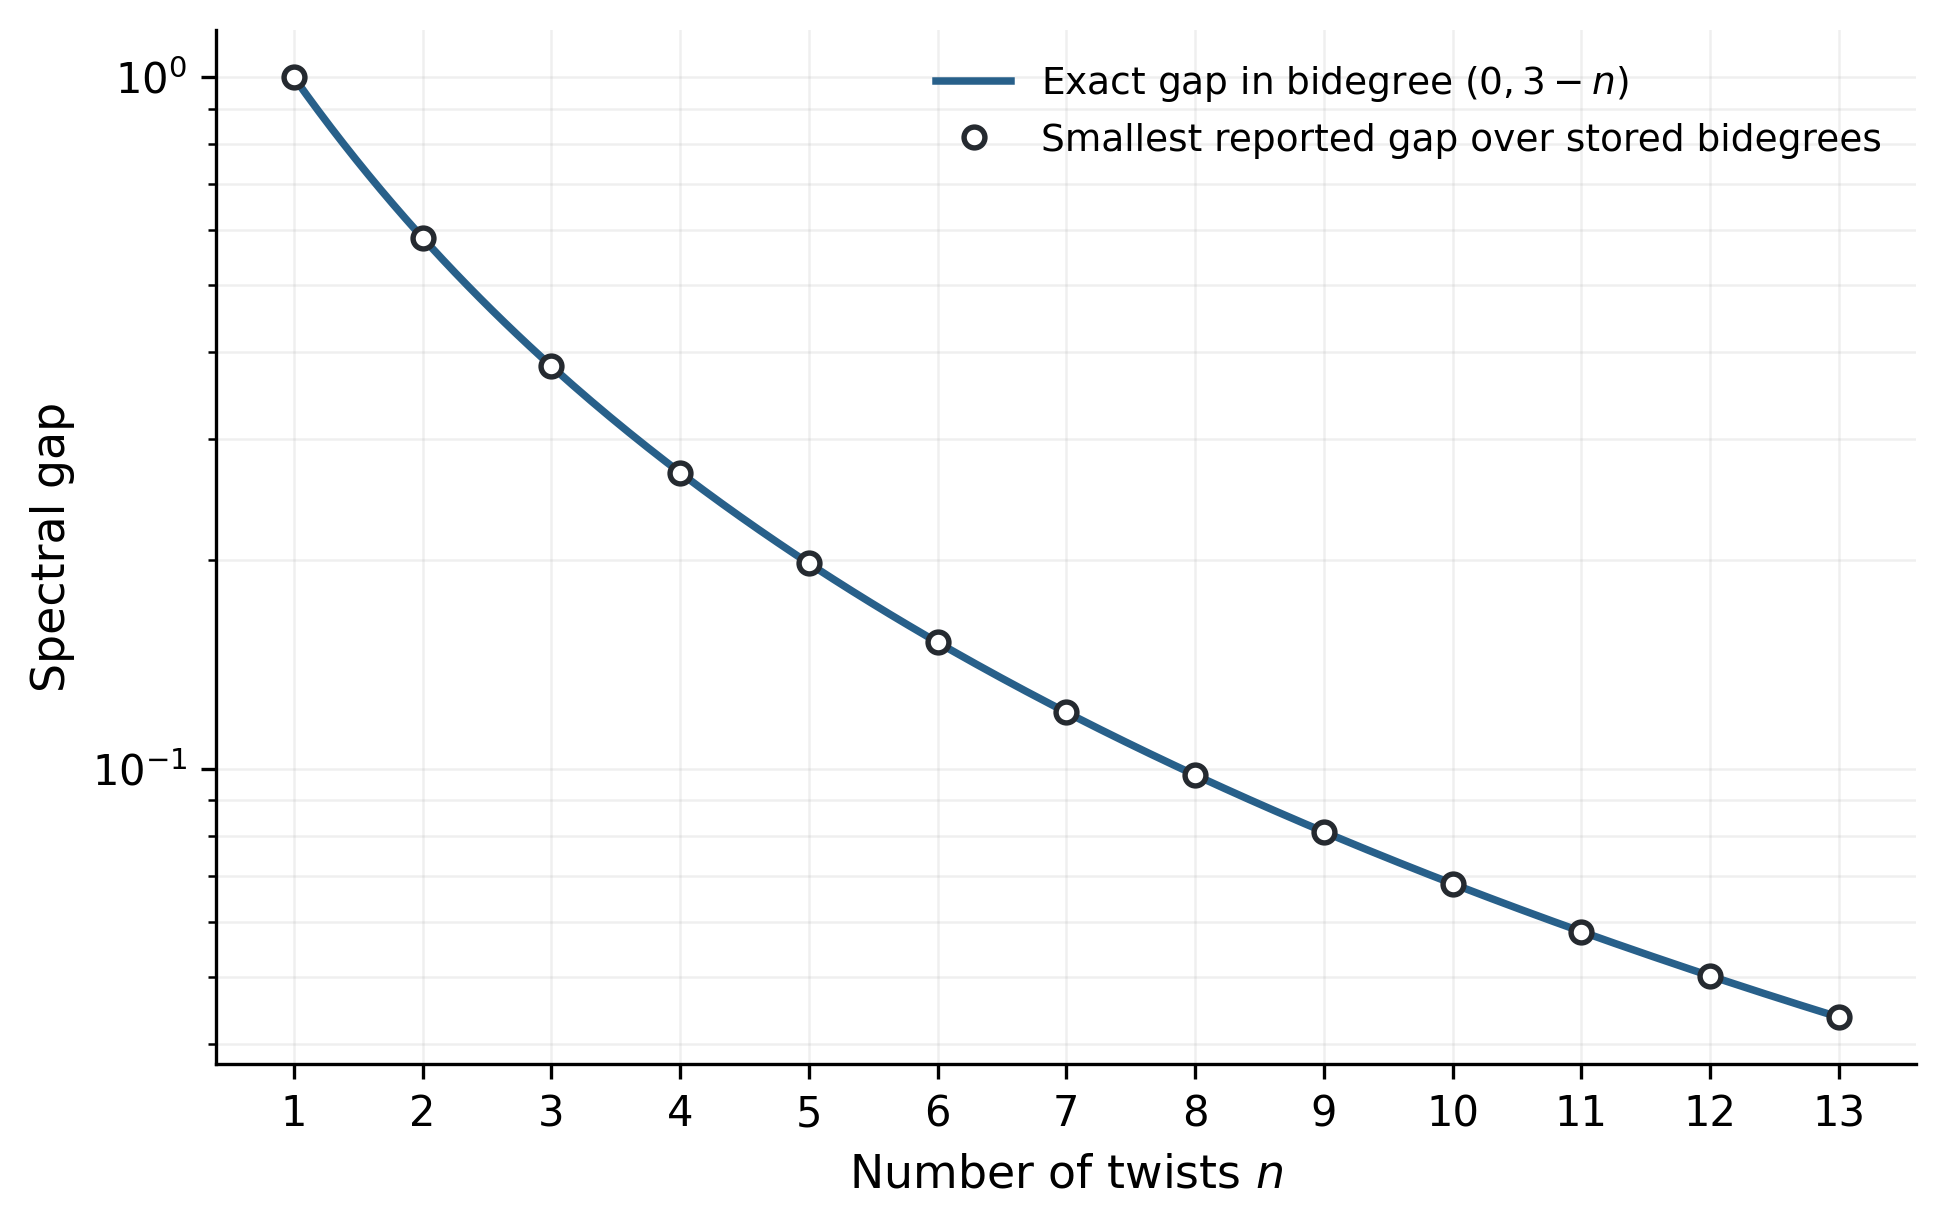
\includegraphics[width=.85\textwidth]{figures/twisted_unknot_bidegree_gap.png}
\caption{Twisted-unknot data and an exact bidegree computation.  Markers are the
smallest stored positive values over the completed bidegrees of $TU_n$; the curve
is the exact value in bidegree $(0,3-n)$.  The two agree throughout the computed
range.}
\label{fig:twists}\label{fig:unknot-plot}
\end{figure}

\subsection{Gap data for fixed KnotInfo and LinkInfo diagrams}
The twisted-unknot family shows that the spectral gap can change under
diagrammatic modifications that preserve the knot type. Thus, for numerical
comparisons, one must fix a diagrammatic representative. We use the PD diagrams
appearing in the KnotInfo and LinkInfo databases for the knots through thirteen
crossings and the links, together with the fourteen-crossing sample
described above.

\Cref{fig:knot_plots,fig:link_plots} show the distribution of
$\widehat\delta(D)$ among completed diagram records.  For knots, the median
decreases from approximately $0.362$ at eight crossings to $0.184$ at thirteen
crossings.  The smallest reported values decrease more strongly, from $0.0530$
to $0.00130$.  For the completed fourteen-crossing subset, the median is
$0.159$ and the smallest reported value is $0.000612$.
The values vary substantially among diagrams with the same crossing number.
The connecting lines are visual guides.

These calculations were performed using the Center for Advanced Research
Computing (CARC) at the University of Southern California.
The cost is driven by the exponential growth of the Khovanov complex with
the crossing number and by the size of the boundary matrices appearing near
the largest diagrams in the dataset.

\begin{figure}[htbp]
\centering
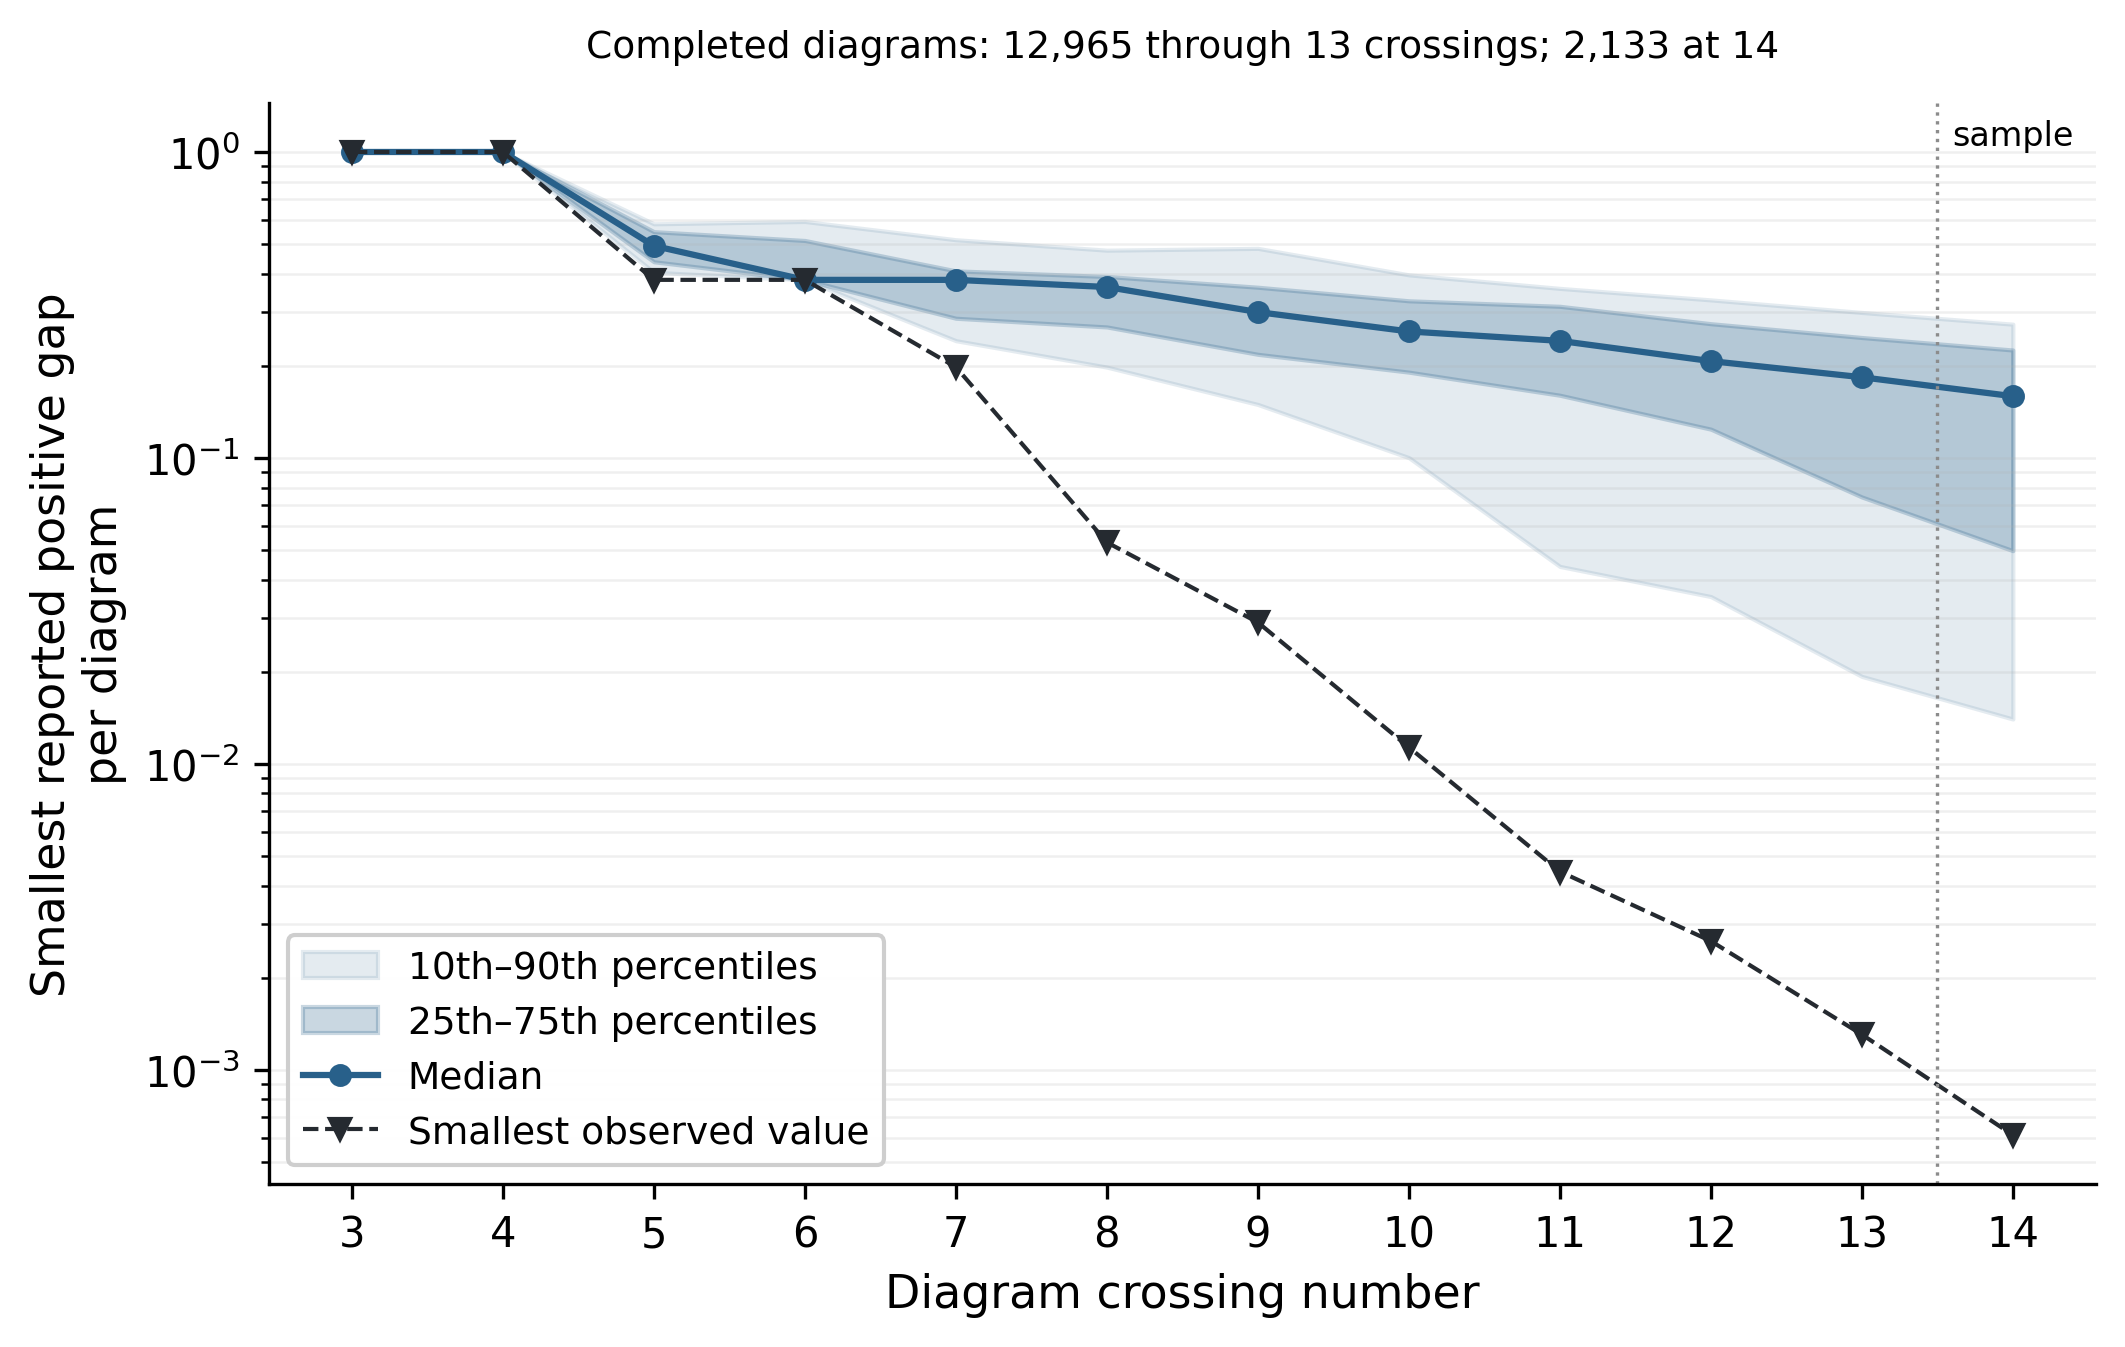
\includegraphics[width=.95\textwidth]{figures/observed_knots_gap_distribution.png}
\caption{One minimum reported positive gap per completed knot diagram.  The
line with circles gives the median, the bands give the central $50\%$ and
$80\%$ of the values, and triangles give the smallest observed value.  Counts
refer to the fixed database snapshot in \Cref{tab:numerical_coverage}.  The
fourteen-crossing column contains the $2{,}133$ completed sample records.}
\label{fig:knot_plots}
\end{figure}

\begin{figure}[htbp]
\centering
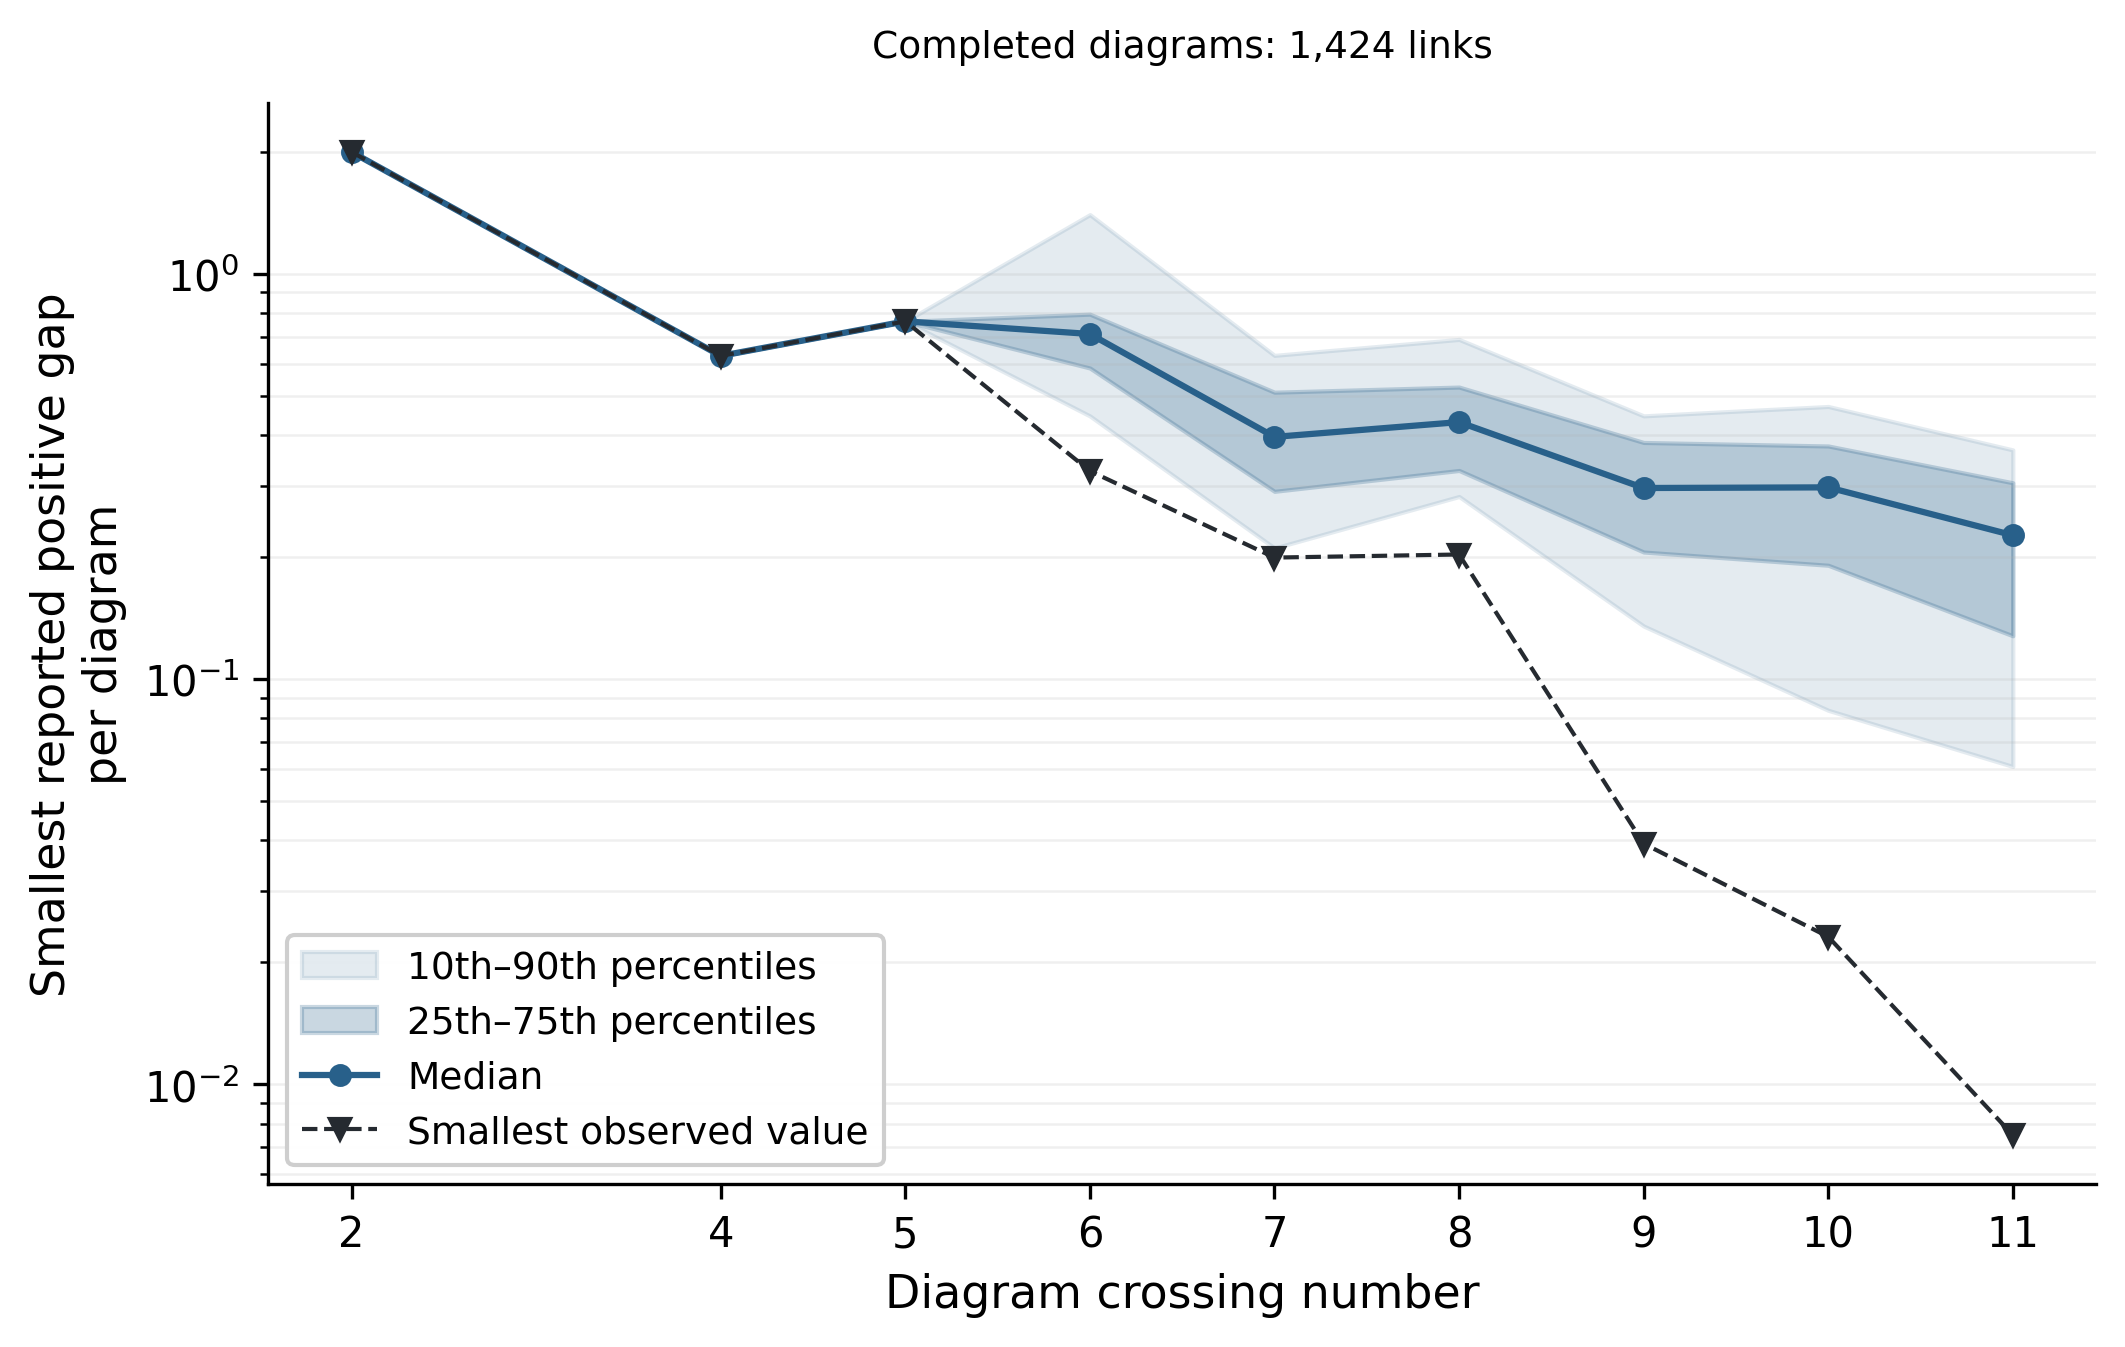
\includegraphics[width=.95\textwidth]{figures/observed_links_gap_distribution.png}
\caption{The same summaries for the $1{,}424$ completed link-diagram records.
Each diagram contributes equally.}
\label{fig:link_plots}
\end{figure}

\Cref{tab:frontier_blocks} lists blocks giving several of the smallest reported
values.  Rebuilding these Laplacian blocks and repeating the calculation
reproduced all ten gap values to within $3\cdot10^{-14}$.

\begin{table}[htbp]
\centering
\begin{tabular}{rllrr}
\hline
$n$ & Diagram & $(h,q)$ & Block dimension & Reported gap \\
\hline
8 & $8_{20}$ & $(0,-3)$ & 165 & $0.052960$ \\
9 & $9_{46}$ & $(-1,-1)$ & 180 & $0.028998$ \\
10 & $10_{153}$ & $(-1,-3)$ & 709 & $0.011328$ \\
11 & $11n_{81}$ & $(6,17)$ & 502 & $0.0044463$ \\
12 & $12n_{723}$ & $(0,-1)$ & 6221 & $0.0026344$ \\
13 & $13n_{2769}$ & $(1,7)$ & 9518 & $0.0013042$ \\
14 & $14nh_{03671}$ & $(0,3)$ & 19336 & $0.00061198$ \\
\hline
9 & $L9n9$ & $(-5,-14)$ & 426 & $0.039259$ \\
10 & $L10n32$ & $(-1,0)$ & 376 & $0.023125$ \\
11 & $L11n71$ & $(-5,-14)$ & 1545 & $0.0074957$ \\
\hline
\end{tabular}
\caption{Blocks attaining the indicated minima in the completed-record sets.
Bidegrees use the shifted Khovanov grading.  The fourteen-crossing identifier
refers to the supplied input table. Every listed diagram is non-alternating.}
\label{tab:frontier_blocks}
\end{table}

Exact rank calculations also show that all ten listed blocks have no zero
modes.  For each block, the ranks of the incoming and outgoing differentials
modulo a prime add to the dimension of the chain space, which implies that
its Betti number over $\mathbb Q$ is zero.

\subsection{Alternating diagrams and exact bidegree formulas}
\label{subsec:alternating_frontier}
The full knot data show a rapidly decreasing minimum, but this behavior is not
visible in the same way after restricting to alternating diagrams
(\Cref{fig:alternating_frontier_placeholder}). For the completed data through
thirteen crossings, the smallest observed spectral gap follows a parity
pattern. At odd crossing numbers through
thirteen, the smallest stored value is attained by the standard two-strand torus
knot diagram $T(2,n)$.  At even crossing numbers through twelve, it agrees with
the distinguished-bidegree value for the standard twist-knot diagram
$\mathrm{Tw}_n$, with $n-2$ crossings in the twist region and two crossings in
the clasp. We index twist knots by their crossing number, following the
conventions of \cite[Definition~4.31]{GrljLaudaSpectralGeometry}. There are ties, for example, $6_1$ and $6_2$ agree at six
crossings, and five diagrams agree at twelve crossings.  The full list of
observed minimizers, using absolute tolerance $10^{-9}$ to identify numerical
ties, is in the derived data table.

For the explicit oriented representatives used
in~\cite[Sections~4.6--4.7]{GrljLaudaSpectralGeometry}---the positive two-strand
braid closure and the specified even twist-knot diagram---the exact results are
\begin{align}
\operatorname{gap}\bigl(\Delta_{n-1,3n-2}(T(2,n))\bigr)
  &=4\sin^2\!\left(\frac{\pi}{2n}\right), &&n\geq3\text{ odd},
\label{eq:torus_distinguished_gap}\\
\operatorname{gap}\bigl(\Delta_{n-2,3n-9}(\mathrm{Tw}_n)\bigr)
  &=4\sin^2\!\left(\frac{\pi}{2(n-1)}\right), &&n\geq4\text{ even},
\label{eq:alternating_distinguished_gaps}
\end{align}
proved in~\cite[Theorems~4.29 and~4.32]{GrljLaudaSpectralGeometry}.
Both gaps are $\Theta(n^{-2})$.

Both alternating branches are governed by the same cycle-graph calculation.
The exact bidegree computations of~\cite[proofs of Theorems~4.29 and~4.32]{GrljLaudaSpectralGeometry} show that,
in the bidegrees just specified, the Khovanov Laplacian is diagonally conjugate
to a cycle-graph operator, up to a rank-one perturbation in the even twist-knot
case. Thus the relevant eigenvalues are obtained from the elementary spectrum
of a cycle.

Let \(C_N\) denote the cycle graph on \(N\) vertices, and let \(A(C_N)\) be
its adjacency matrix. The eigenvalues of \(A(C_N)\) are
\[
2\cos\left(\frac{2\pi j}{N}\right),
\qquad j=0,\ldots,N-1 .
\]
For the torus-knot branch, the relevant operator is \(2I+A(C_n)\). Since
\(n\) is odd, its smallest eigenvalue is
\[
2-2\cos\left(\frac{\pi}{n}\right)
=
4\sin^2\left(\frac{\pi}{2n}\right).
\]
For the even twist-knot branch, the conjugated Laplacian is the
rank-one perturbation \(2I+A(C_{n-1})+uu^{\mathsf T}\) with \(u=e_1+e_2\).
Since \(n-1\) is odd, the smallest eigenvalue of \(2I+A(C_{n-1})\) is
\(4\sin^2\!\left(\frac{\pi}{2(n-1)}\right)\), and its two-dimensional
eigenspace contains a vector orthogonal to \(u\), so the minimum is
unchanged by the perturbation. In both cases the gap in the distinguished
bidegree decays quadratically in the crossing-number parameter.

At thirteen crossings, the smallest observed alternating gap is
$0.058116\ldots$, attained by $T(2,13)=13a_{4878}$.  This agrees
with the formula in bidegree $(12,37)$ for the positive two-strand braid
representative.  Among the $886$ alternating diagrams in the fourteen-crossing
sample, the smallest reported value is $0.086549\ldots$, attained by
$14ah_{00033}$.  The exact bidegree value for the standard twist diagram
$\mathrm{Tw}_{14}$ is shown separately for comparison in
\Cref{fig:alternating_frontier_placeholder}.

\begin{figure}[htbp]
\centering
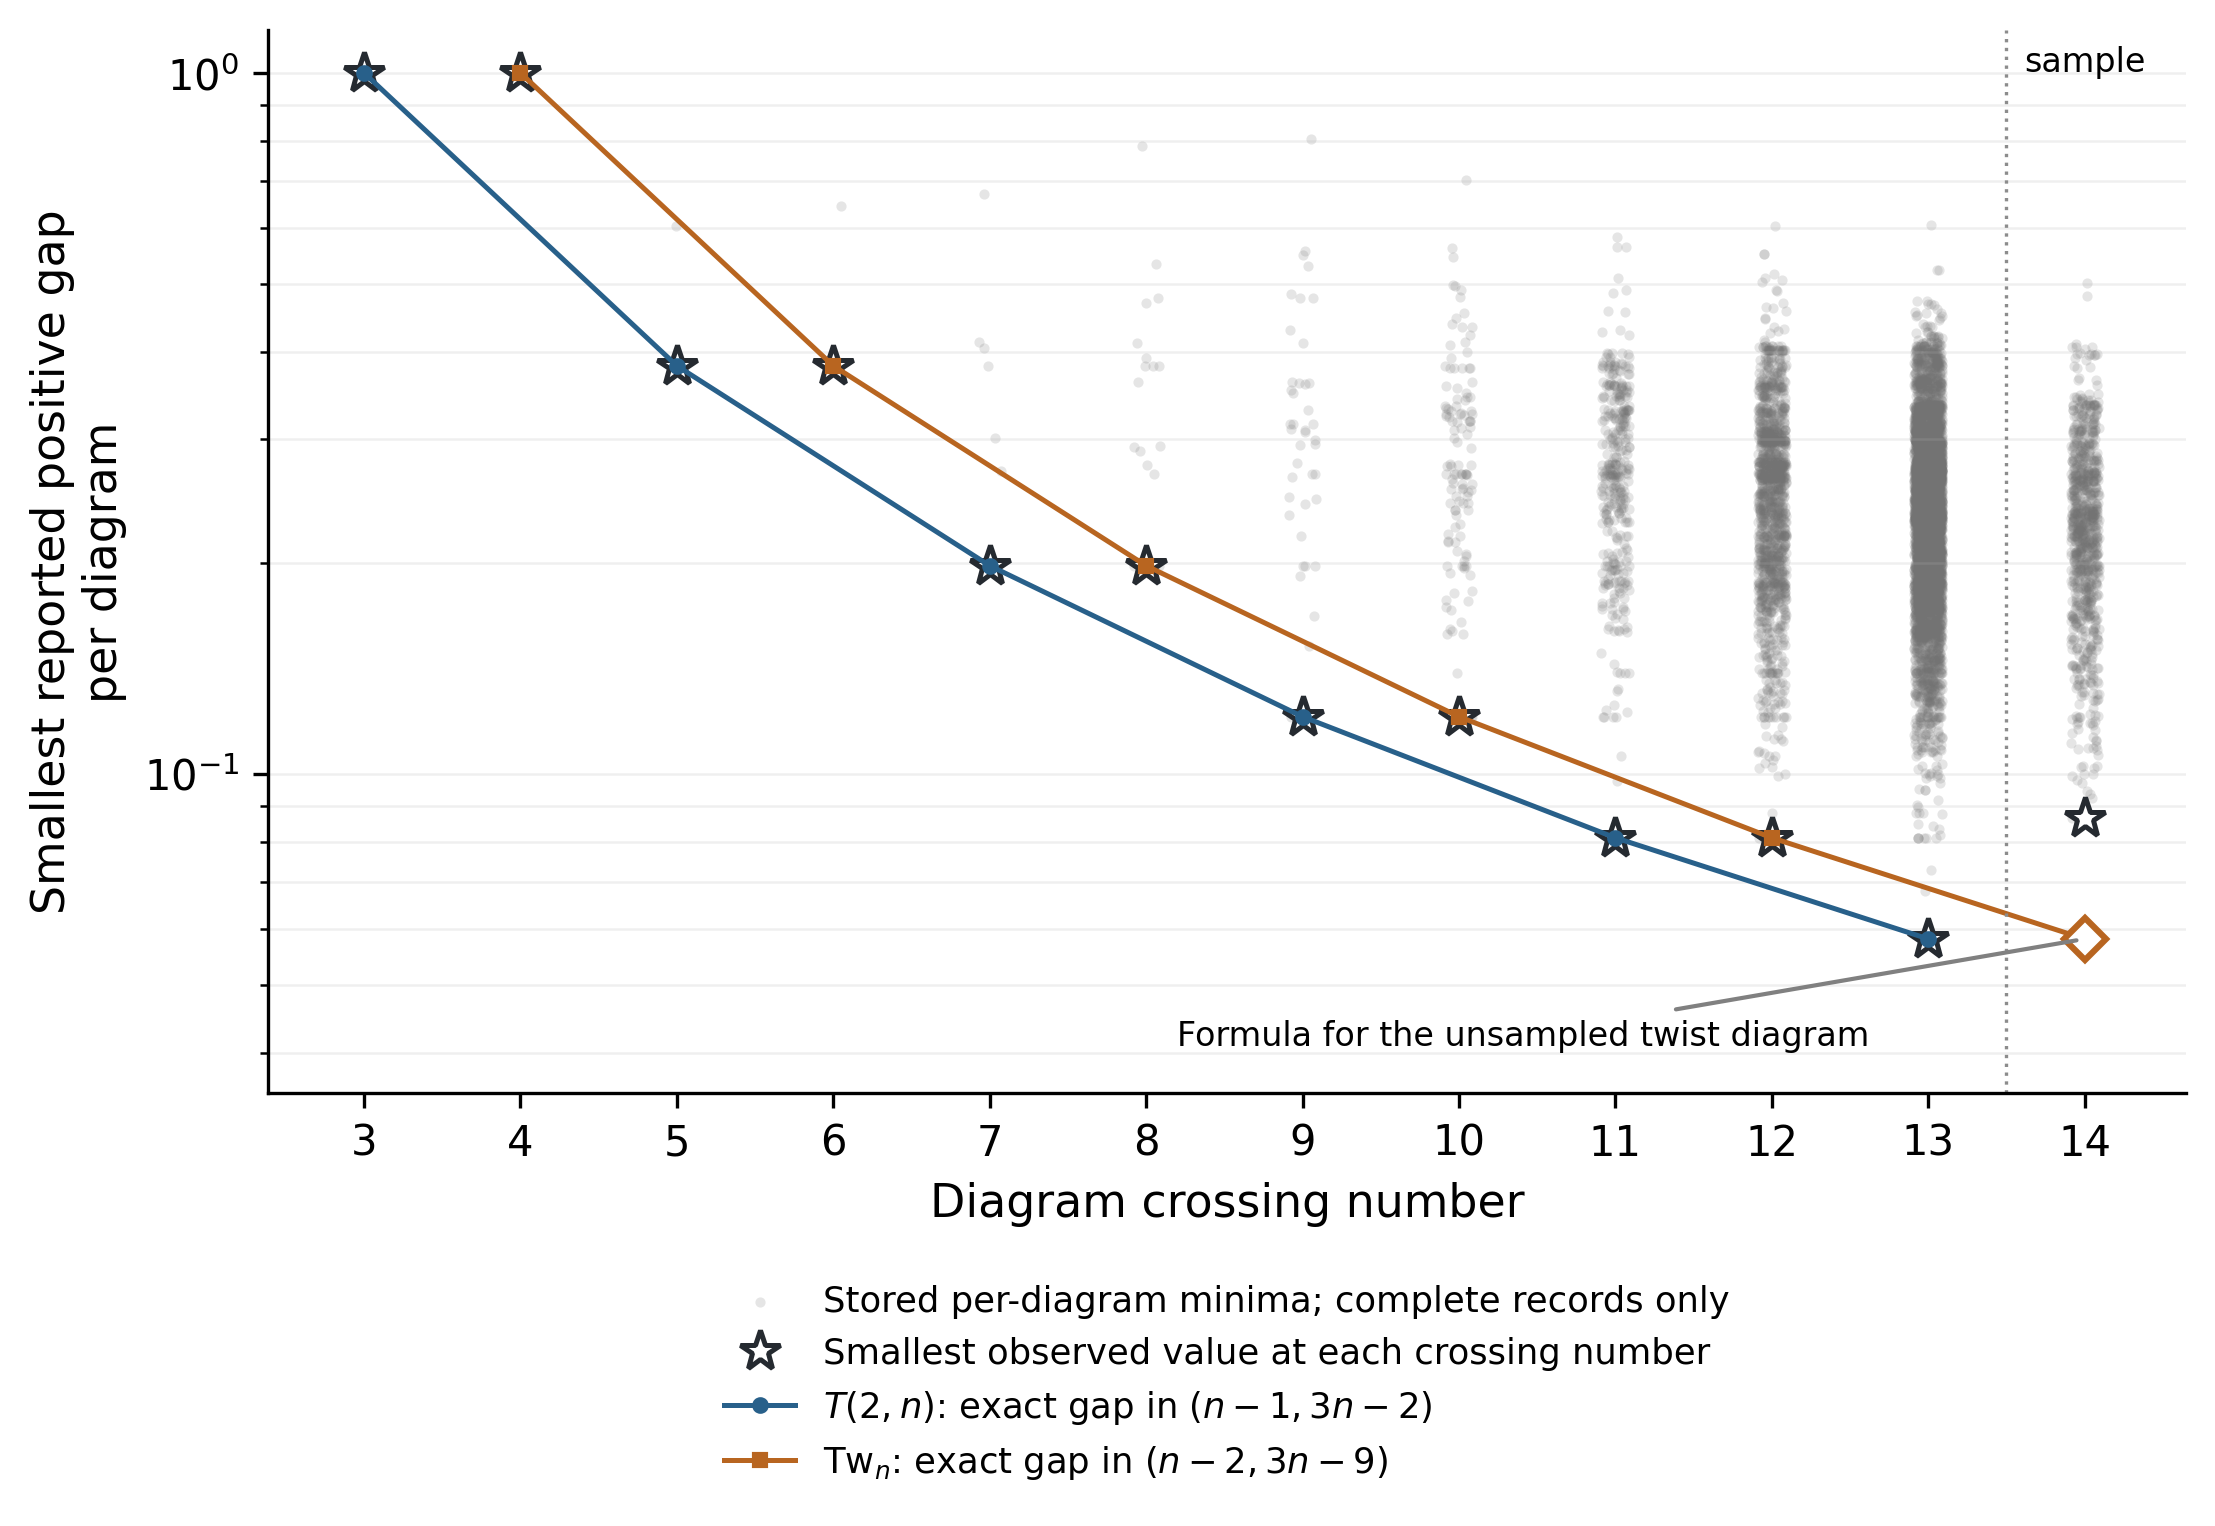
\includegraphics[width=.95\textwidth]{figures/alternating_distinguished_bidegrees.png}
\caption{Alternating-diagram data and exact distinguished-bidegree formulas.
Gray points give the per-diagram gaps and stars give their minimum at each
crossing number, using completed records.  Curves give the formulas in
\Cref{eq:torus_distinguished_gap,eq:alternating_distinguished_gaps}.
The open diamond gives the exact bidegree value for $\mathrm{Tw}_{14}$,
shown for comparison with the fourteen-crossing sample.}
\label{fig:alternating_frontier_placeholder}
\label{fig:alternating_frontier_families}
\end{figure}

The Gibbs-state protocol also needs a low-temperature state with adequate overlap
with the kernel and uniform weights within it. In alternating diagrams the spanning-tree
construction also gives a classical benchmark, whose efficiency does not
require a gap bound for the full-chain Laplacian.
% ===================== END numerics.tex =====================


% ==================== BEGIN spanning.tex ====================
\section{Spanning-tree initialization and the alternating benchmark}
\label{sec:spanning_trees}

The spectral data above address the spectral-resolution bottleneck. The alternating-only data suggest that alternating diagrams form a more regular test class, while the overall smallest gap in the present dataset comes from a non-alternating knot. We now discuss the spanning-tree construction as a source of structured initial states for the Khovanov Hodge Laplacian. In alternating diagrams the same construction also gives a classical benchmark.

The spanning-tree constructions of Wehrli and Champanerkar--Kofman compute Khovanov homology using a smaller complex built from a graph associated with the diagram \cite{wehrli2004spanningtree,champanerkar2008spanningtrees,ChampanerkarKofmanMutation2008}.

\subsection{From a diagram to a spanning-tree complex}

Fix a connected oriented link diagram \(D\) with \(m\) crossings and a marked point away from the crossings. Choose a checkerboard shading of \(D\). The associated \emph{Tait graph} \(G_D\) is obtained by placing a vertex in each shaded region and an edge across each crossing joining the two adjacent shaded regions. Loops and parallel edges are allowed. We write \(\mathrm{ST}(G_D)\) for the set of spanning trees of \(G_D\), and \(\tau(G_D)\) for their number. \Cref{fig:taitgraph} illustrates the construction.

For the activity grading we use the checkerboard signs of \cite{champanerkar2008spanningtrees}. An edge is positive if the Kauffman \(A\)-smoothing joins the adjacent shaded regions, and negative if the \(B\)-smoothing does so. Here \(A\) and \(B\) denote the \(0\)- and \(1\)-smoothings, respectively, in \cref{eq:skein}. These edge signs do not use a link orientation and differ from the oriented crossing signs that determine \(n_\pm\) and the writhe \(w=n_+-n_-\). Switching the shading replaces the graph by its planar dual and reverses its edge signs. We choose a shading with at least as many positive as negative edges. For an alternating diagram one of the two choices makes every edge positive.

\begin{figure}[t]
\centering
$%% HOPF LINK WITH SHADE
 \begin{tikzpicture}[scale=.4] 
    \fill[fill=gray!50, even odd rule, thick]
  (-1,2.5) .. controls +(0,3) and +(0,3) .. (4,2.5)
         .. controls +(0,-.25) and +(0,.25) ..  (3,1.5)
         .. controls +(0,-.75)  and  +(.5,-.75)..  (2,1) 
         .. controls +(0,.25) and +(0,-.25) .. (1,2)
         .. controls +(0,.25) and +(0,-.25) .. (2,3)
         .. controls +(.5,.75) and +(0,.75) .. (3,2.5)
         .. controls +(0,-.25) and +(0,.25) .. (4,1.5) 
         .. controls +(0,-3) and +(0,-3) .. (-1,1.5) 
         .. controls +(0,.25) and +(0,-.25) .. (0,2.5)
          .. controls  +(0,.75) and  +(-.5,.75).. (1,3)
          .. controls +(0,-.25) and +(0,.25) .. (2,2) 
           .. controls +(0,-.25) and +(0,.25) .. (1,1)
           .. controls +(-.5,-.75) and +(0,-.75) .. (0,1.5)
           .. controls +(0,.25) and +(0,-.25) .. (-1,2.5)
         -- cycle;

  \draw [black, very thick]    (2,1) .. controls +(0,.25) and +(0,-.25) .. (1,2);
  \draw [black, very thick]    (2,2) .. controls +(0,.25) and +(0,-.25) .. (1,3);
  \path [fill=gray!50] (1.35,1) rectangle (1.65,3);
  \draw [black, very thick]    (1,1) .. controls +(0,.25) and +(0,-.25) .. (2,2);
  \draw [black, very thick]    (1,2) .. controls +(0,.25) and +(0,-.25) .. (2,3);
  \draw [black, very thick]    (2,3) .. controls +(.5,.75) and +(0,.75) .. (3,2.5); 
  \draw [black, very thick]    (2,1) .. controls +(.5,-.75) and +(0,-.75) .. (3,1.5); 
  \draw [black, very thick]    (1,3) .. controls +(-.5,.75) and +(0,.75) .. (0,2.5); 
  \draw [black, very thick]    (1,1) .. controls +(-.5,-.75) and +(0,-.75) .. (0,1.5); 
  \draw [black, very thick]    (3,1.5) .. controls +(0,.25) and +(0,-.25) .. (4,2.5);
  \path [fill=gray!50] (3.35,1.5) rectangle (3.65,2.5);
  \draw [black, very thick]    (4,1.5) .. controls +(0,.25) and +(0,-.25) .. (3,2.5); 
  \draw [black, very thick]    (-1,1.5) .. controls +(0,.25) and +(0,-.25) .. (0,2.5);
  \path [fill=gray!50] (-0.35,1.5) rectangle (-0.65,2.5);
  \draw [black, very thick]    (0,1.5) .. controls +(0,.25) and +(0,-.25) .. (-1,2.5); 
  \draw [black, very thick]    (-1,2.5) .. controls +(0,3) and +(0,3) .. (4,2.5); 
  \draw [black, very thick]    (-1,1.5) .. controls +(0,-3) and +(0,-3) .. (4,1.5); 
\node at (-1.5,2) {$\scriptstyle \underline{1}$};
\node at (1.5,3.25) {$\scriptstyle\underline{2}$};
\node at (1.5,.75) {$\scriptstyle\underline{3}$};
\node at (4.5,2) {$\scriptstyle\underline{4}$};
    \end{tikzpicture}
    \quad 
 \begin{tikzpicture}[scale=.4] 
    \fill[fill=gray!50, even odd rule, thick]
  (-1,2.5) .. controls +(0,3) and +(0,3) .. (4,2.5)
         .. controls +(0,-.25) and +(0,.25) ..  (3,1.5)
         .. controls +(0,-.75)  and  +(.5,-.75)..  (2,1) 
         .. controls +(0,.25) and +(0,-.25) .. (1,2)
         .. controls +(0,.25) and +(0,-.25) .. (2,3)
         .. controls +(.5,.75) and +(0,.75) .. (3,2.5)
         .. controls +(0,-.25) and +(0,.25) .. (4,1.5) 
         .. controls +(0,-3) and +(0,-3) .. (-1,1.5) 
         .. controls +(0,.25) and +(0,-.25) .. (0,2.5)
          .. controls  +(0,.75) and  +(-.5,.75).. (1,3)
          .. controls +(0,-.25) and +(0,.25) .. (2,2) 
           .. controls +(0,-.25) and +(0,.25) .. (1,1)
           .. controls +(-.5,-.75) and +(0,-.75) .. (0,1.5)
           .. controls +(0,.25) and +(0,-.25) .. (-1,2.5)
         -- cycle;
  \draw [black, very thick]    (2,1) .. controls +(0,.25) and +(0,-.25) .. (1,2);
  \draw [black, very thick]    (2,2) .. controls +(0,.25) and +(0,-.25) .. (1,3);
  \path [fill=gray!50] (1.35,1) rectangle (1.65,3);
  \draw [black, very thick]    (1,1) .. controls +(0,.25) and +(0,-.25) .. (2,2);
  \draw [black, very thick]    (1,2) .. controls +(0,.25) and +(0,-.25) .. (2,3);
  \draw [black, very thick]    (2,3) .. controls +(.5,.75) and +(0,.75) .. (3,2.5); 
  \draw [black, very thick]    (2,1) .. controls +(.5,-.75) and +(0,-.75) .. (3,1.5); 
  \draw [black, very thick]    (1,3) .. controls +(-.5,.75) and +(0,.75) .. (0,2.5); 
  \draw [black, very thick]    (1,1) .. controls +(-.5,-.75) and +(0,-.75) .. (0,1.5); 
  \draw [black, very thick]    (3,1.5) .. controls +(0,.25) and +(0,-.25) .. (4,2.5);
  \path [fill=gray!50] (3.35,1.5) rectangle (3.65,2.5);
  \draw [black, very thick]    (4,1.5) .. controls +(0,.25) and +(0,-.25) .. (3,2.5); 
  \draw [black, very thick]    (-1,1.5) .. controls +(0,.25) and +(0,-.25) .. (0,2.5);
  \path [fill=gray!50] (-0.35,1.5) rectangle (-0.65,2.5);
  \draw [black, very thick]    (0,1.5) .. controls +(0,.25) and +(0,-.25) .. (-1,2.5); 
  \draw [black, very thick]    (-1,2.5) .. controls +(0,3) and +(0,3) .. (4,2.5); 
  \draw [black, very thick]    (-1,1.5) .. controls +(0,-3) and +(0,-3) .. (4,1.5); 
  \coordinate (T) at (1.5,4);
  \coordinate (M) at (1.5,2);
  \coordinate (B) at (1.5,0);

  \draw[thick, blue] (T) -- (B); % Straight middle edge
  \draw[thick, blue] (T) .. controls +(-2.7, 0) and +(-2.7, 0) .. (B);
  \draw[thick, blue] (T) .. controls +(2.7, 0) and +(2.7, 0) .. (B);% 

  \fill[blue] (T) circle (0.15);
  \fill[blue] (B) circle (0.15);
  \fill[blue] (M) circle (0.15);
    \end{tikzpicture}
\quad  
\begin{tikzpicture}[scale=.4] 
  \coordinate (T) at (1.5,4);
  \coordinate (M) at (1.5,2);
  \coordinate (B) at (1.5,0);

  \draw[thick, blue] (T) -- (B); % Straight middle edge
  \draw[thick, blue] (T) .. controls +(-2.4, 0) and +(-2.4, 0) .. (B);
  \draw[thick, blue] (T) .. controls +(2.4, 0) and +(2.4, 0) .. (B);% 

  \fill[blue] (T) circle (0.2);
  \fill[blue] (B) circle (0.2);
  \fill[blue] (M) circle (0.2);
\node[blue] at (-1.0,2) {$\scriptstyle 1$};
\node[blue] at (1.2,3) {$\scriptstyle 2$};
\node[blue] at (1.2,1) {$\scriptstyle 3$};
\node[blue] at (4.0,2) {$\scriptstyle 4$};
\node at (0,-1.4) {$\;$};
    \end{tikzpicture} $

\caption{A checkerboard shading of a link diagram and the associated Tait graph. Vertices are placed in the shaded regions and edges cross the crossings adjacent to those regions. The final picture records the same graph without the diagram. The labels identify crossings; the checkerboard signs described in the text are omitted here.}
\label{fig:taitgraph}
\end{figure}

Thistlethwaite's spanning-tree expansion expresses the Jones polynomial as a sum over spanning trees of \(G_D\) \cite{This}. Every spanning tree corresponds to a partial resolution of \(D\) that is a twisted unknot, meaning an unknot diagram obtained from the simple unknot by repeated Reidemeister-I moves. \Cref{fig:spanningtree} shows this correspondence for the trefoil. The full cube has \(2^3\) complete resolutions, while the spanning-tree expansion stops at the twisted unknot leaves.

The connection between spanning trees and twisted unknots is encoded by activity words \cite{This}. Once an ordering of the crossings is fixed, the activity word of a spanning tree records which crossings are resolved and which crossings remain as Reidemeister-I twists. An edge \(e\) in a spanning tree \(T\) is \emph{internally active}, or live, if it is the least edge in the cut determined by removing \(e\) from \(T\). An edge \(f\) outside \(T\) is \emph{externally active}, or live, if it is the least edge in the cycle of \(T\cup f\). Other edges are called dead. For a loop the latter cycle consists just of that loop; a bridge belongs to every spanning tree. Crossings corresponding to dead edges are smoothed, and those corresponding to live edges remain as twists in the diagram \(U(T)\).

\begin{figure}[t]
    \centering
\resizebox{\linewidth}{!}{%
$
\begin{tikzpicture}
 \node (000) at (-3.5 ,0) {
    \begin{tikzpicture}[scale=.25] 
      \draw [black, very thick]    (2,1) -- (2,2); 
      \draw [black, very thick]    (1,1) -- (1,2);
      \draw [black, very thick]    (2,2) -- (2,4); 
      \draw [black, very thick]    (1,2) -- (1,4);
      \draw [black, very thick]    (1,4) .. controls +(-.1,.5) and +(+.1,.5) .. (0,4);
      \draw [black, very thick]    (2,4) .. controls +(+.1,.5) and +(-.1,.5) .. (3,4);
      \draw [black, very thick]    (0,4) -- (0,1);
      \draw [black, very thick]    (3,4) -- (3,1);
      \draw [black, very thick]    (1,1) .. controls +(-0.1,-0.5) and+(+0.1,-0.5) .. (0,1);
      \draw [black, very thick]    (2,1) .. controls +(0.1,-0.5) and +(-0.1,-0.5) .. (3,1);
        \end{tikzpicture}
  };
  \node (001) at (-2.5,0) {
    \begin{tikzpicture}[scale=.25] 
      \draw [black, very thick]    (2,2) -- (2,3); 
      \draw [black, very thick]    (1,2) -- (1,3);
      \draw [black, very thick]    (2,1) .. controls +(0,.35) and +(0,.35) ..(1,1); 
      \draw [black, very thick]    (1,2) .. controls +(0,-.35) and +(0,-.35) .. (2,2);
      \draw [black, very thick]    (2,3) -- (2,4); 
      \draw [black, very thick]    (1,3) -- (1,4);
      \draw [black, very thick]    (1,4) .. controls +(-.1,.5) and +(+.1,.5) .. (0,4);
      \draw [black, very thick]    (2,4) .. controls +(+.1,.5) and +(-.1,.5) .. (3,4);
      \draw [black, very thick]    (0,4) -- (0,1);
      \draw [black, very thick]    (3,4) -- (3,1);
      \draw [black, very thick]    (1,1) .. controls +(-0.1,-0.5) and+(+0.1,-0.5) .. (0,1);
      \draw [black, very thick]    (2,1) .. controls +(0.1,-0.5) and +(-0.1,-0.5) .. (3,1);
        \end{tikzpicture}
  };
    \node (010) at (-1.5,0) {
    \begin{tikzpicture}[scale=.25] 
      \draw [black, very thick]    (2,1) -- (2,2); 
      \draw [black, very thick]    (1,1) -- (1,2);
      \draw [black, very thick]    (2,2) .. controls +(0,.35) and +(0,.35) ..(1,2); 
      \draw [black, very thick]    (1,3) .. controls +(0,-.35) and +(0,-.35) .. (2,3);
      \draw [black, very thick]    (2,3) -- (2,4); 
      \draw [black, very thick]    (1,3) -- (1,4);
      \draw [black, very thick]    (1,4) .. controls +(-.1,.5) and +(+.1,.5) .. (0,4);
      \draw [black, very thick]    (2,4) .. controls +(+.1,.5) and +(-.1,.5) .. (3,4);
      \draw [black, very thick]    (0,4) -- (0,1);
      \draw [black, very thick]    (3,4) -- (3,1);
      \draw [black, very thick]    (1,1) .. controls +(-0.1,-0.5) and+(+0.1,-0.5) .. (0,1);
      \draw [black, very thick]    (2,1) .. controls +(0.1,-0.5) and +(-0.1,-0.5) .. (3,1);
        \end{tikzpicture}
  };
   \node (011) at (-.5,0) {
    \begin{tikzpicture}[scale=.25] 
      \draw [black, very thick]    (2,1) .. controls +(0,.35) and +(0,.35) ..(1,1); 
      \draw [black, very thick]    (1,2) .. controls +(0,-.35) and +(0,-.35) .. (2,2);
      \draw [black, very thick]    (2,2) .. controls +(0,.35) and +(0,.35) ..(1,2); 
      \draw [black, very thick]    (1,3) .. controls +(0,-.35) and +(0,-.35) .. (2,3);
      \draw [black, very thick]    (2,3) -- (2,4); 
      \draw [black, very thick]    (1,3) -- (1,4);
      \draw [black, very thick]    (1,4) .. controls +(-.1,.5) and +(+.1,.5) .. (0,4);
      \draw [black, very thick]    (2,4) .. controls +(+.1,.5) and +(-.1,.5) .. (3,4);
      \draw [black, very thick]    (0,4) -- (0,1);
      \draw [black, very thick]    (3,4) -- (3,1);
      \draw [black, very thick]    (1,1) .. controls +(-0.1,-0.5) and+(+0.1,-0.5) .. (0,1);
      \draw [black, very thick]    (2,1) .. controls +(0.1,-0.5) and +(-0.1,-0.5) .. (3,1);
        \end{tikzpicture}
   };
    \node (100) at (.5,0) {
    \begin{tikzpicture}[scale=.25] 
      \draw [black, very thick]    (2,1) -- (2,2); 
      \draw [black, very thick]    (1,1) -- (1,2);
      \draw [black, very thick]    (2,2) -- (2,3); 
      \draw [black, very thick]    (1,2) -- (1,3);
      \draw [black, very thick]    (2,3) .. controls +(0,.35) and +(0,.35) ..(1,3); 
      \draw [black, very thick]    (1,4) .. controls +(0,-.35) and +(0,-.35) .. (2,4);
      \draw [black, very thick]    (1,4) .. controls +(-.1,.5) and +(+.1,.5) .. (0,4);
      \draw [black, very thick]    (2,4) .. controls +(+.1,.5) and +(-.1,.5) .. (3,4);
      \draw [black, very thick]    (0,4) -- (0,1);
      \draw [black, very thick]    (3,4) -- (3,1);
      \draw [black, very thick]    (1,1) .. controls +(-0.1,-0.5) and+(+0.1,-0.5) .. (0,1);
      \draw [black, very thick]    (2,1) .. controls +(0.1,-0.5) and +(-0.1,-0.5) .. (3,1);
        \end{tikzpicture}
    };
    \node (101) at (1.5,0) {
    \begin{tikzpicture}[scale=.25] 
      \draw [black, very thick]    (2,1) .. controls +(0,.35) and +(0,.35) .. (1,1);
      \draw [black, very thick]    (1,2) -- (1,3);
      \draw [black, very thick]    (2,3) .. controls +(0,.35) and +(0,.35) .. (1,3);
      \draw [black, very thick]    (1,2) .. controls +(0,-.35) and +(0,-.35) .. (2,2);
      \draw [black, very thick]    (2,2)  -- (2,3);
        \draw [black, very thick]    (1,4) .. controls +(0,-.35) and +(0,-.35) .. (2,4);
      \draw [black, very thick]    (1,4) .. controls +(-.1,.5) and +(+.1,.5) .. (0,4);
      \draw [black, very thick]    (2,4) .. controls +(+.1,.5) and +(-.1,.5) .. (3,4);
      \draw [black, very thick]    (0,4) -- (0,1);
      \draw [black, very thick]    (3,4) -- (3,1);
      \draw [black, very thick]    (1,1) .. controls +(-0.1,-0.5) and+(+0.1,-0.5) .. (0,1);
      \draw [black, very thick]    (2,1) .. controls +(0.1,-0.5) and +(-0.1,-0.5) .. (3,1);
        \end{tikzpicture}
    };
    \node (110) at (2.5,0) {
    \begin{tikzpicture}[scale=.25] 
      \draw [black, very thick]    (2,1) -- (2,2);
      \draw [black, very thick]    (2,3) .. controls +(0,.35) and +(0,.35) .. (1,3);
      \draw [black, very thick]    (2,3) .. controls +(0,-.35) and +(0,-.35) .. (1,3);
      \draw [black, very thick]    (1,1) -- (1,2);
      \draw [black, very thick]    (1,2) .. controls +(0,.35) and +(0,.35) .. (2,2);
        \draw [black, very thick]    (1,4) .. controls +(0,-.35) and +(0,-.35) .. (2,4);
      \draw [black, very thick]    (1,4) .. controls +(-.1,.5) and +(+.1,.5) .. (0,4);
      \draw [black, very thick]    (2,4) .. controls +(+.1,.5) and +(-.1,.5) .. (3,4);
      \draw [black, very thick]    (0,4) -- (0,1);
      \draw [black, very thick]    (3,4) -- (3,1);
      \draw [black, very thick]    (1,1) .. controls +(-0.1,-0.5) and+(+0.1,-0.5) .. (0,1);
      \draw [black, very thick]    (2,1) .. controls +(0.1,-0.5) and +(-0.1,-0.5) .. (3,1);
        \end{tikzpicture}
    };
    \node (111) at (3.5,0) {
    \begin{tikzpicture}[scale=.25] 
      \draw [black, very thick]    (2,1) .. controls +(0,.35) and +(0,.35) .. (1,1);
      \draw [black, very thick]    (2,3) .. controls +(0,.35) and +(0,.35) .. (1,3);
      \draw [black, very thick]    (2,3) .. controls +(0,-.35) and +(0,-.35) .. (1,3);
      \draw [black, very thick]    (1,2) .. controls +(0,-.35) and +(0,-.35) .. (2,2);
      \draw [black, very thick]    (1,2) .. controls +(0,.35) and +(0,.35) .. (2,2);
        \draw [black, very thick]    (1,4) .. controls +(0,-.35) and +(0,-.35) .. (2,4);
      \draw [black, very thick]    (1,4) .. controls +(-.1,.5) and +(+.1,.5) .. (0,4);
      \draw [black, very thick]    (2,4) .. controls +(+.1,.5) and +(-.1,.5) .. (3,4);
      \draw [black, very thick]    (0,4) -- (0,1);
      \draw [black, very thick]    (3,4) -- (3,1);
      \draw [black, very thick]    (1,1) .. controls +(-0.1,-0.5) and+(+0.1,-0.5) .. (0,1);
      \draw [black, very thick]    (2,1) .. controls +(0.1,-0.5) and +(-0.1,-0.5) .. (3,1);
        \end{tikzpicture}
    };
    \node (00X) at (-3,1.6) {
    \begin{tikzpicture}[scale=.25] 
     \draw [black, very thick]    (2,1) .. controls +(0,.25) and +(0,-.25) .. (1,2);
      \path [fill=white] (1.35,1) rectangle (1.65,2);
      \draw [black, very thick]    (1,1) .. controls +(0,.25) and +(0,-.25) .. (2,2);
      \draw [black, very thick]    (2,2) -- (2,4); 
      \draw [black, very thick]    (1,2) -- (1,4);
      \draw [black, very thick]    (1,4) .. controls +(-.1,.5) and +(+.1,.5) .. (0,4);
      \draw [black, very thick]    (2,4) .. controls +(+.1,.5) and +(-.1,.5) .. (3,4);
      \draw [black, very thick]    (0,4) -- (0,1);
      \draw [black, very thick]    (3,4) -- (3,1);
      \draw [black, very thick]    (1,1) .. controls +(-0.1,-0.5) and+(+0.1,-0.5) .. (0,1);
      \draw [black, very thick]    (2,1) .. controls +(0.1,-0.5) and +(-0.1,-0.5) .. (3,1);
        \end{tikzpicture}
    };
    \node (01X) at (-1,1.6) {
    \begin{tikzpicture}[scale=.25] 
        \draw [black, very thick]    (2,1) .. controls +(0,.25) and +(0,-.25) .. (1,2);
      \path [fill=white] (1.35,1) rectangle (1.65,2);
      \draw [black, very thick]    (1,1) .. controls +(0,.25) and +(0,-.25) .. (2,2);
      \draw [black, very thick]    (2,2) .. controls +(0,.35) and +(0,.35) ..(1,2); 
      \draw [black, very thick]    (1,3) .. controls +(0,-.35) and +(0,-.35) .. (2,3);
      \draw [black, very thick]    (2,3) -- (2,4); 
      \draw [black, very thick]    (1,3) -- (1,4);
      \draw [black, very thick]    (1,4) .. controls +(-.1,.5) and +(+.1,.5) .. (0,4);
      \draw [black, very thick]    (2,4) .. controls +(+.1,.5) and +(-.1,.5) .. (3,4);
      \draw [black, very thick]    (0,4) -- (0,1);
      \draw [black, very thick]    (3,4) -- (3,1);
      \draw [black, very thick]    (1,1) .. controls +(-0.1,-0.5) and+(+0.1,-0.5) .. (0,1);
      \draw [black, very thick]    (2,1) .. controls +(0.1,-0.5) and +(-0.1,-0.5) .. (3,1);
        \end{tikzpicture}
    };
    \node (10X) at (1,1.6) {
    \begin{tikzpicture}[scale=.25] 
      \draw [black, very thick]    (2,1) .. controls +(0,.25) and +(0,-.25) .. (1,2);
      \path [fill=white] (1.35,1) rectangle (1.65,2);
      \draw [black, very thick]    (1,1) .. controls +(0,.25) and +(0,-.25) .. (2,2);
      \draw [black, very thick]    (2,2) -- (2,3); 
      \draw [black, very thick]    (1,2) -- (1,3);
      \draw [black, very thick]    (2,3) .. controls +(0,.35) and +(0,.35) ..(1,3); 
      \draw [black, very thick]    (1,4) .. controls +(0,-.35) and +(0,-.35) .. (2,4);
      \draw [black, very thick]    (1,4) .. controls +(-.1,.5) and +(+.1,.5) .. (0,4);
      \draw [black, very thick]    (2,4) .. controls +(+.1,.5) and +(-.1,.5) .. (3,4);
      \draw [black, very thick]    (0,4) -- (0,1);
      \draw [black, very thick]    (3,4) -- (3,1);
      \draw [black, very thick]    (1,1) .. controls +(-0.1,-0.5) and+(+0.1,-0.5) .. (0,1);
      \draw [black, very thick]    (2,1) .. controls +(0.1,-0.5) and +(-0.1,-0.5) .. (3,1);
        \end{tikzpicture}
    };
    \node (11X) at (3,1.6) {
    \begin{tikzpicture}[scale=.25] 
      \draw [black, very thick]    (2,1) .. controls +(0,.25) and +(0,-.25) .. (1,2);
      \path [fill=white] (1.35,1) rectangle (1.65,2);
      \draw [black, very thick]    (1,1) .. controls +(0,.25) and +(0,-.25) .. (2,2);
      \draw [black, very thick]    (2,3) .. controls +(0,.35) and +(0,.35) .. (1,3);
      \draw [black, very thick]    (2,3) .. controls +(0,-.35) and +(0,-.35) .. (1,3);
      \draw [black, very thick]    (1,2) .. controls +(0,.35) and +(0,.35) .. (2,2);
        \draw [black, very thick]    (1,4) .. controls +(0,-.35) and +(0,-.35) .. (2,4);
      \draw [black, very thick]    (1,4) .. controls +(-.1,.5) and +(+.1,.5) .. (0,4);
      \draw [black, very thick]    (2,4) .. controls +(+.1,.5) and +(-.1,.5) .. (3,4);
      \draw [black, very thick]    (0,4) -- (0,1);
      \draw [black, very thick]    (3,4) -- (3,1);
      \draw [black, very thick]    (1,1) .. controls +(-0.1,-0.5) and+(+0.1,-0.5) .. (0,1);
      \draw [black, very thick]    (2,1) .. controls +(0.1,-0.5) and +(-0.1,-0.5) .. (3,1);
        \end{tikzpicture}
    };
    \node (0XX) at (-2,3.2) {
    \begin{tikzpicture}[scale=.25] 
     \draw [black, very thick]    (2,1) .. controls +(0,.25) and +(0,-.25) .. (1,2);
      \path [fill=white] (1.35,1) rectangle (1.65,2);
      \draw [black, very thick]    (1,1) .. controls +(0,.25) and +(0,-.25) .. (2,2);
      \draw [black, very thick]    (2,2) .. controls +(0,.25) and +(0,-.25) .. (1,3);
      \path [fill=white] (1.35,2) rectangle (1.65,3);
      \draw [black, very thick]    (1,2) .. controls +(0,.25) and +(0,-.25) .. (2,3);
      \draw [black, very thick]    (2,3) -- (2,4); 
      \draw [black, very thick]    (1,3) -- (1,4);
      \draw [black, very thick]    (1,4) .. controls +(-.1,.5) and +(+.1,.5) .. (0,4);
      \draw [black, very thick]    (2,4) .. controls +(+.1,.5) and +(-.1,.5) .. (3,4);
      \draw [black, very thick]    (0,4) -- (0,1);
      \draw [black, very thick]    (3,4) -- (3,1);
      \draw [black, very thick]    (1,1) .. controls +(-0.1,-0.5) and+(+0.1,-0.5) .. (0,1);
      \draw [black, very thick]    (2,1) .. controls +(0.1,-0.5) and +(-0.1,-0.5) .. (3,1);
        \end{tikzpicture}
    };
    \node (1XX) at (2,3.2) {
    \begin{tikzpicture}[scale=.25] 
      \draw [black, very thick]    (2,1) .. controls +(0,.25) and +(0,-.25) .. (1,2);
      \path [fill=white] (1.35,1) rectangle (1.65,2);
      \draw [black, very thick]    (1,1) .. controls +(0,.25) and +(0,-.25) .. (2,2);
      \draw [black, very thick]    (2,2) .. controls +(0,.25) and +(0,-.25) .. (1,3);
      \path [fill=white] (1.35,2) rectangle (1.65,3);
      \draw [black, very thick]    (1,2) .. controls +(0,.25) and +(0,-.25) .. (2,3);
      \draw [black, very thick]    (2,3) .. controls +(0,.35) and +(0,.35) ..(1,3); 
      \draw [black, very thick]    (1,4) .. controls +(0,-.35) and +(0,-.35) .. (2,4);
      \draw [black, very thick]    (1,4) .. controls +(-.1,.5) and +(+.1,.5) .. (0,4);
      \draw [black, very thick]    (2,4) .. controls +(+.1,.5) and +(-.1,.5) .. (3,4);
      \draw [black, very thick]    (0,4) -- (0,1);
      \draw [black, very thick]    (3,4) -- (3,1);
      \draw [black, very thick]    (1,1) .. controls +(-0.1,-0.5) and+(+0.1,-0.5) .. (0,1);
      \draw [black, very thick]    (2,1) .. controls +(0.1,-0.5) and +(-0.1,-0.5) .. (3,1);
        \end{tikzpicture}
    };
    \node (XXX) at (0,3.8) {
    \begin{tikzpicture}[scale=.25] 
     \draw [black, very thick]    (2,1) .. controls +(0,.25) and +(0,-.25) .. (1,2);
      \path [fill=white] (1.35,1) rectangle (1.65,2);
      \draw [black, very thick]    (1,1) .. controls +(0,.25) and +(0,-.25) .. (2,2);
      \draw [black, very thick]    (2,2) .. controls +(0,.25) and +(0,-.25) .. (1,3);
      \path [fill=white] (1.35,2) rectangle (1.65,3);
      \draw [black, very thick]    (1,2) .. controls +(0,.25) and +(0,-.25) .. (2,3);
      \draw [black, very thick]    (2,3) .. controls +(0,.25) and +(0,-.25) .. (1,4);
      \path [fill=white] (1.35,3) rectangle (1.65,4);
      \draw [black, very thick]    (1,3) .. controls +(0,.25) and +(0,-.25) .. (2,4);
      \draw [black, very thick]    (1,4) .. controls +(-.1,.5) and +(+.1,.5) .. (0,4);
      \draw [black, very thick]    (2,4) .. controls +(+.1,.5) and +(-.1,.5) .. (3,4);
      \draw [black, very thick]    (0,4) -- (0,1);
      \draw [black, very thick]    (3,4) -- (3,1);
      \draw [black, very thick]    (1,1) .. controls +(-0.1,-0.5) and+(+0.1,-0.5) .. (0,1);
      \draw [black, very thick]    (2,1) .. controls +(0.1,-0.5) and +(-0.1,-0.5) .. (3,1);
        \end{tikzpicture}
    };
    \draw [thick,-] (XXX) -- node[above]{$0\;$} (0XX);
    \draw [thick,-] (XXX) -- node[above]{$1\;$} (1XX);
    \draw [thick,-] (0XX) -- node[left]{$0$} (00X);
    \draw [thick,-] (0XX) -- node[right]{$1$} (01X);
    \draw [thick,-] (1XX) -- node[left]{$0$} (10X);
    \draw [thick,-] (1XX) -- node[right]{$1$} (11X);
    \draw [thick,-] (00X) -- node[left]{$0$} (000);
    \draw [thick,-] (00X) -- node[right]{$1$} (001);
    \draw [thick,-] (01X) -- node[left]{$0$} (010);
    \draw [thick,-] (01X) -- node[right]{$1$} (011);
    \draw [thick,-] (10X) -- node[left]{$0$} (100);
    \draw [thick,-] (10X) -- node[right]{$1$} (101);
    \draw [thick,-] (11X) -- node[left]{$0$} (110);
    \draw [thick,-] (11X) -- node[right]{$1$} (111);
\end{tikzpicture}
\qquad 
\begin{tikzpicture}
\node  at (-3.7,2.0) {
    \begin{tikzpicture}[scale=.2] 
      \coordinate (L) at (0.5,2.5);
      \coordinate (R) at (2.5,2.5);
    
      \draw[thick, blue] (L) .. controls +(0.0, -1.3) and +(0, -1.3) .. node[below]{$\scriptstyle  3$} (R) ; % Bottom curved edge
    
      \fill[blue] (L) circle (0.25);
      \fill[blue] (R) circle (0.25);
          \end{tikzpicture}
};
\node  at (-.2,2.0) {
    \begin{tikzpicture}[scale=.2] 
      \coordinate (L) at (0.5,2.5);
      \coordinate (R) at (2.5,2.5);
    
     \draw[thick, blue] (L) -- node[below]{$\scriptstyle  2$}(R); % Straight middle edge
    
      \fill[blue] (L) circle (0.25);
      \fill[blue] (R) circle (0.25);
            \end{tikzpicture}
};
\node  at (0,5.0) {
    \begin{tikzpicture}[scale=.3] 
      \coordinate (L) at (0.5,2.5);
      \coordinate (R) at (2.5,2.5);
    
      \draw[thick, blue] (L) -- node[below=-1.9pt]{$\scriptscriptstyle  2$} (R); % Straight middle edge
      \draw[thick, blue] (L) .. controls +(0.0, 1.3) and +(0, 1.3) .. node[above ]{$\scriptscriptstyle  1$} (R); % Top 
      \draw[thick, blue] (L) .. controls +(0.0, -1.3) and +(0, -1.3) .. node[below=-1.9pt]{$\scriptscriptstyle  3$}(R); % Bottom curved edge
    
      \fill[blue] (L) circle (0.25);
      \fill[blue] (R) circle (0.25);
            \end{tikzpicture}
};
\node  at (3,3.8) {
    \begin{tikzpicture}[scale=.25] 
      \coordinate (L) at (0.5,2.5);
      \coordinate (R) at (2.5,2.5);
    \draw[thick, blue] (L) .. controls +(0.0, 1.3) and +(0, 1.3) .. node[above ]{$\scriptscriptstyle  1$} (R); % Top 
      \fill[blue] (L) circle (0.25);
      \fill[blue] (R) circle (0.25);
    \end{tikzpicture}
};
    \node (00X) at (-3,1.6) {
\begin{tikzpicture}[scale=.25] 
  \fill[fill=gray!50, even odd rule, thick]
    (0,1) .. controls +(-0.1,-0.5) and+(+0.1,-0.5) ..  (1,1)
          .. controls +(0,.25) and +(0,-.25) .. (2,2)
           -- (2,4)
           .. controls +(+.1,.5) and +(-.1,.5) .. (3,4)
            -- (3,1)
            .. controls +(-0.1,-0.5) and +(0.1,-0.5) .. (2,1)
            .. controls +(0,.25) and +(0,-.25) .. (1,2)
            -- (1,4)
            .. controls +(-.1,.5) and +(+.1,.5) .. (0,4)
            -- cycle;
            
  \draw [black, very thick]    (2,1) .. controls +(0,.25) and +(0,-.25) .. (1,2);
  \draw [black, very thick]    (2,2) -- (2,4);
  \path [fill=white] (1.35,1) rectangle (1.65,4);
  \draw [black, very thick]    (1,1) .. controls +(0,.25) and +(0,-.25) .. (2,2);
    \draw [black, very thick]    (1,2) -- (1,4);
  \draw [black, very thick]    (1,4) .. controls +(-.1,.5) and +(+.1,.5) .. (0,4);
  \draw [black, very thick]    (2,4) .. controls +(+.1,.5) and +(-.1,.5) .. (3,4);
  \draw [black, very thick]    (0,4) -- (0,1);
  \draw [black, very thick]    (3,4) -- (3,1);
  \draw [black, very thick]    (1,1) .. controls +(-0.1,-0.5) and+(+0.1,-0.5) .. (0,1);
  \draw [black, very thick]    (2,1) .. controls +(0.1,-0.5) and +(-0.1,-0.5) .. (3,1);

      \end{tikzpicture}
    };
    \node (01X) at (-1,1.6) {
\begin{tikzpicture}[scale=.25] 
  \fill[fill=gray!50, even odd rule, thick]
    (0,1)  .. controls +(0.1,-0.5) and+(-0.1,-0.5) ..(1,1)
            .. controls +(0,.25) and +(0,-.25) .. (2,2)
            .. controls +(0,.35) and +(0,.35) .. (1,2)
            
               .. controls +(0,-.25) and +(0,.25) .. (2,1) 
               .. controls +(0.1,-0.5) and +(-0.1,-0.5) .. (3,1)
               -- (3,4)
                .. controls +(-.1,.5) and +(.1,.5) ..(2,4)
                -- (2,3)
                .. controls +(0,-.35) and +(0,-.35) .. (1,3)
                -- (1,4)
                .. controls +(-.1,.5) and +(+.1,.5) .. (0,4)
            -- cycle;
            
  \draw [black, very thick]    (2,1) .. controls +(0,.25) and +(0,-.25) .. (1,2);
  \draw [black, very thick]    (2,3) .. controls +(0,-.35) and +(0,-.35) .. (1,3);
  \draw [black, very thick]    (2,3) -- (2,4);
  \path [fill=white] (1.35,1) rectangle (1.65,2);
  \draw [black, very thick]    (1,1) .. controls +(0,.25) and +(0,-.25) .. (2,2);
  \draw [black, very thick]    (1,2) .. controls +(0,.35) and +(0,.35) .. (2,2);
    \draw [black, very thick]    (1,3) -- (1,4);
  \draw [black, very thick]    (1,4) .. controls +(-.1,.5) and +(+.1,.5) .. (0,4);
  \draw [black, very thick]    (2,4) .. controls +(+.1,.5) and +(-.1,.5) .. (3,4);
  \draw [black, very thick]    (0,4) -- (0,1);
  \draw [black, very thick]    (3,4) -- (3,1);
  \draw [black, very thick]    (1,1) .. controls +(-0.1,-0.5) and+(+0.1,-0.5) .. (0,1);
  \draw [black, very thick]    (2,1) .. controls +(0.1,-0.5) and +(-0.1,-0.5) .. (3,1);

      \end{tikzpicture}
    };
    \node (0XX) at (-2,3.2) {
\begin{tikzpicture}[scale=.25] 
  \fill[fill=gray!50, even odd rule, thick]
    (0,1) .. controls +(-0.1,-0.5) and+(+0.1,-0.5) ..  (1,1)
          .. controls +(0,.25) and +(0,-.25) .. (2,2)
           .. controls +(0,.25) and +(0,-.25) .. (1,3)
           -- (1,4) 
          .. controls +(-.1,.5) and +(+.1,.5) .. (0,4)
            -- cycle 
            
    (3,1) .. controls +(-0.1,-0.5) and +(0.1,-0.5) .. (2,1)
            .. controls +(0,.25) and +(0,-.25) .. (1,2)
            .. controls +(0,.25) and +(0,-.25) .. (2,3)
            -- (2,4)
             .. controls +(+.1,.5) and +(-.1,.5) .. (3,4)
            --  cycle; 
            
  \draw [black, very thick]    (2,1) .. controls +(0,.25) and +(0,-.25) .. (1,2);
  \draw [black, very thick]    (2,2) .. controls +(0,.25) and +(0,-.25) .. (1,3);
  \draw [black, very thick]    (2,3) -- (2,4);
  \path [fill=white] (1.35,1) rectangle (1.65,4);
  \draw [black, very thick]    (1,1) .. controls +(0,.25) and +(0,-.25) .. (2,2);
  \draw [black, very thick]    (1,2) .. controls +(0,.25) and +(0,-.25) .. (2,3);
    \draw [black, very thick]    (1,3) -- (1,4);
  \draw [black, very thick]    (1,4) .. controls +(-.1,.5) and +(+.1,.5) .. (0,4);
  \draw [black, very thick]    (2,4) .. controls +(+.1,.5) and +(-.1,.5) .. (3,4);
  \draw [black, very thick]    (0,4) -- (0,1);
  \draw [black, very thick]    (3,4) -- (3,1);
  \draw [black, very thick]    (1,1) .. controls +(-0.1,-0.5) and+(+0.1,-0.5) .. (0,1);
  \draw [black, very thick]    (2,1) .. controls +(0.1,-0.5) and +(-0.1,-0.5) .. (3,1);
    \end{tikzpicture}
    };
    \node (1XX) at (2,3.2) {
    \begin{tikzpicture}[scale=.25] 
      \fill[fill=gray!50, even odd rule, thick]
        (0,1)  .. controls +(0.1,-0.5) and+(-0.1,-0.5) ..(1,1)
                .. controls +(0,.25) and +(0,-.25) .. (2,2)
                 .. controls +(0,.25) and +(0,-.25) .. (1,3)
                  .. controls +(0,.35) and +(0,.35) .. (2,3)
                   .. controls +(0,-.25) and +(0,.25) .. (1,2)
                   .. controls +(0,-.25) and +(0,.25) .. (2,1) 
                   .. controls +(0.1,-0.5) and +(-0.1,-0.5) .. (3,1)
                   -- (3,4)
                    .. controls +(-.1,.5) and +(.1,.5) ..(2,4)
                    .. controls +(0,-.35) and +(0,-.35) .. (1,4) 
                    .. controls +(-.1,.5) and +(+.1,.5) .. (0,4)
                -- cycle;
      \draw [black, very thick]    (2,1) .. controls +(0,.25) and +(0,-.25) .. (1,2);
      \draw [black, very thick]    (2,2) .. controls +(0,.25) and +(0,-.25) .. (1,3);
      \draw [black, very thick]    (2,3) .. controls +(0,.35) and +(0,.35) .. (1,3);
      \path [fill=white] (1.35,1) rectangle (1.65,3);
      \draw [black, very thick]    (1,1) .. controls +(0,.25) and +(0,-.25) .. (2,2);
      \draw [black, very thick]    (1,2) .. controls +(0,.25) and +(0,-.25) .. (2,3);
        \draw [black, very thick]    (1,4) .. controls +(0,-.35) and +(0,-.35) .. (2,4);
      \draw [black, very thick]    (1,4) .. controls +(-.1,.5) and +(+.1,.5) .. (0,4);
      \draw [black, very thick]    (2,4) .. controls +(+.1,.5) and +(-.1,.5) .. (3,4);
      \draw [black, very thick]    (0,4) -- (0,1);
      \draw [black, very thick]    (3,4) -- (3,1);
      \draw [black, very thick]    (1,1) .. controls +(-0.1,-0.5) and+(+0.1,-0.5) .. (0,1);
      \draw [black, very thick]    (2,1) .. controls +(0.1,-0.5) and +(-0.1,-0.5) .. (3,1);
    
          \end{tikzpicture}
    };
    \node (XXX) at (0,3.8) {
    \begin{tikzpicture}[scale=.25] 
  \fill[fill=gray!50, even odd rule, thick]
    (0,1) .. controls +(-0.1,-0.5) and+(+0.1,-0.5) ..  (1,1)
          .. controls +(0,.25) and +(0,-.25) .. (2,2)
           .. controls +(0,.25) and +(0,-.25) .. (1,3)
           .. controls +(0,.25) and +(0,-.25) .. (2,4)
           .. controls +(+.1,.5) and +(-.1,.5) .. (3,4)
            -- (3,1)
            .. controls +(-0.1,-0.5) and +(0.1,-0.5) .. (2,1)
            .. controls +(0,.25) and +(0,-.25) .. (1,2)
            .. controls +(0,.25) and +(0,-.25) .. (2,3)
            .. controls +(0,.25) and +(0,-.25) .. (1,4)
            .. controls +(-.1,.5) and +(+.1,.5) .. (0,4)
            -- cycle;
  \draw [black, very thick]    (2,1) .. controls +(0,.25) and +(0,-.25) .. (1,2);
  \draw [black, very thick]    (2,2) .. controls +(0,.25) and +(0,-.25) .. (1,3);
  \draw [black, very thick]    (2,3) .. controls +(0,.25) and +(0,-.25) .. (1,4);
  \path [fill=white] (1.35,1) rectangle (1.65,4);
  \draw [black, very thick]    (1,1) .. controls +(0,.25) and +(0,-.25) .. (2,2);
  \draw [black, very thick]    (1,2) .. controls +(0,.25) and +(0,-.25) .. (2,3);
    \draw [black, very thick]    (1,3) .. controls +(0,.25) and +(0,-.25) .. (2,4);
  \draw [black, very thick]    (1,4) .. controls +(-.1,.5) and +(+.1,.5) .. (0,4);
  \draw [black, very thick]    (2,4) .. controls +(+.1,.5) and +(-.1,.5) .. (3,4);
  \draw [black, very thick]    (0,4) -- (0,1);
  \draw [black, very thick]    (3,4) -- (3,1);
  \draw [black, very thick]    (1,1) .. controls +(-0.1,-0.5) and+(+0.1,-0.5) .. (0,1);
  \draw [black, very thick]    (2,1) .. controls +(0.1,-0.5) and +(-0.1,-0.5) .. (3,1);

  

    \end{tikzpicture}
    };
    \draw [thick,-] (XXX) -- node[above]{$0\;$} (0XX);
    \draw [thick,-] (XXX) -- node[above]{$1\;$} (1XX);
    \draw [thick,-] (0XX) -- node[left]{$0$} (00X);
    \draw [thick,-] (0XX) -- node[right]{$1$} (01X); 
\end{tikzpicture}$
}% end scaled resolution tree
    \caption{The trefoil's full resolution tree (left) and its spanning-tree expansion (right). The full expansion has eight complete resolutions; the pruned expansion has three leaves, each a twisted unknot. The shaded Tait graph is the theta graph, with one spanning tree for each of its three edges. Reversing the shading gives the dual triangle; both choices have the same number of spanning trees.}
    \label{fig:spanningtree}
\end{figure}

In the spanning-tree models of Wehrli and Champanerkar--Kofman, the activity word also determines the bidegree of the associated generator. In the reduced theory there is one generator per tree. Let \(L,\ell\) count the positive live edges inside and outside \(T\), and let \(\bar L,\bar\ell\) denote the analogous negative live edges. Put
\[
 u(T)=L-\ell-\bar L+\bar\ell,\qquad v(T)=E_+(T),
\]
where \(E_+(T)\) is the number of positive edges in the tree. The reduced spanning-tree complex has one generator for each tree and a differential of bidegree \((-1,-1)\) in \((u,v)\). It is a deformation retract of the reduced complex of the marked link \cite[Theorem 3]{champanerkar2008spanningtrees}, \cite[Theorem 2]{ChampanerkarKofmanMutation2008}. In the reduced convention of \Cref{subsec:Kh-bracket-homology}, with the unknot in bidegree \((0,-1)\), define
\[
 \kappa=E_+(G_D)-E_-(G_D)+2\bigl(|V(G_D)|-1\bigr).
\]
The corresponding Khovanov bidegree is
\begin{align}
 i(T)&=u(T)-2v(T)+\frac{w+\kappa}{2}, \nonumber\\
 j(T)&=2u(T)-2v(T)+\frac{3w+\kappa}{2}-1 .
 \label{eq:tree-gradings}
\end{align}
This is the inverse of the grading change in \cite[eq.~(1)]{champanerkar2008spanningtrees}. Cut and cycle tests compute the activities, and hence \((i(T),j(T))\), in polynomial time. The unreduced model instead has two generators per tree; its differential need not vanish even for an alternating diagram.

\subsection{A direct classical estimator for alternating links}

For an alternating diagram, the reduced spanning-tree differential vanishes for grading reasons \cite[Theorem 7 and Remark 1]{champanerkar2008spanningtrees}. Every spanning tree in the all-positive Tait graph of a connected diagram has \(v(T)=|V(G_D)|-1\). Because the differential changes \(v\), it must vanish. Consequently, uniform spanning-tree sampling gives an unbiased estimator for the normalized reduced Betti distribution.

\begin{theorem}[Alternating reduced spanning-tree estimator]
\label{thm:alternating-tree-estimator}
Let \(D\) be a connected alternating diagram of a link \(L\), with a chosen basepoint, and take coefficients in \(\mathbb C\). Then
\[
 \widetilde\beta_{i,j}(L)
 =\#\{T\in\mathrm{ST}(G_D):(i(T),j(T))=(i,j)\},
 \qquad
 \sum_{i,j}\widetilde\beta_{i,j}(L)=\tau(G_D).
\]
The total reduced rank is computable exactly in deterministic polynomial time. For \(0<\varepsilon,\nu<1\), independent uniform spanning-tree samples give simultaneous estimates of every
\[
 p_{i,j}:=\widetilde\beta_{i,j}(L)/\tau(G_D)
\]
to additive error \(\varepsilon\), with failure probability at most \(\nu\), in expected time polynomial in \(m,\varepsilon^{-1},\log\nu^{-1}\).
\end{theorem}

\begin{proof}
The vanishing differential identifies reduced homology with the spanning-tree generators in their bidegrees, proving the counting identities. The matrix-tree theorem computes \(\tau(G_D)\) as a determinant of a graph-Laplacian minor \cite{Kirchhoff1847,KleeStamps2019}; its integer entries and result have polynomial bit length.

For the sampling statement, enclose all possible bidegrees in the explicitly computable rectangle
\[
 \mathcal R(D)=
 \{-n_-,\ldots,n_+\}\times
 \{s-\ell_0,\ldots,s+m+\ell_1\},
 \qquad s=n_+-2n_-,
\]
where \(\ell_0,\ell_1\) are the loop counts of the all-\(0\) and all-\(1\) resolutions. Every reduced generator has a bidegree occurring in the full reduced complex, so this rectangle contains its support. Its cardinality
\(M=(m+1)(m+\ell_0+\ell_1+1)=O((m+1)^2)\) is known without enumerating the support.

If \(T_1,\ldots,T_N\) are independent uniform trees, set
\[
 \widehat p_{i,j}=\frac1N\sum_{a=1}^N
 \mathbf1\{(i(T_a),j(T_a))=(i,j)\}.
\]
These estimates are unbiased. Hoeffding's inequality and a union bound imply
\[
 \Pr\!\left[\max_{(i,j)\in\mathcal R(D)}
 |\widehat p_{i,j}-p_{i,j}|>\varepsilon\right]
 \le 2M e^{-2N\varepsilon^2}.
\]
Thus \(N\ge(2\varepsilon^2)^{-1}\log(2M/\nu)\) suffices. Wilson's loop-erased random-walk algorithm samples an exact uniform spanning tree of this finite unweighted connected graph in expected polynomial time \cite{Wilson96}. The activity grading is polynomial-time computable.
\end{proof}

With the tree basis declared orthonormal, the reduced spanning-tree Laplacian is identically zero. Consequently its uniform mixture satisfies
\[
 \widetilde\rho_{\mathrm{ST}}
 =\frac1{\tau(G_D)}\sum_T |T\rangle\langle T|
 =\frac{\widetilde\Pi_0}{\tau(G_D)}.
\]
It is already exactly maximally mixed on its kernel. No full-chain gap, harmonic overlap, Gibbs preparation, or bound on the size of an individual Betti number enters \Cref{thm:alternating-tree-estimator}.

The positive trefoil uses the all-positive triangle, not its all-negative theta dual. Here \(w=3\), \(\kappa=7\), \(v=2\), and the three activities give \(u=-1,1,2\). Formula \cref{eq:tree-gradings} yields reduced generators in bidegrees \((0,1),(2,5),(3,7)\). Their Euler characteristic is \(q+q^5-q^7=q^{-1}V_{3_1}(q^2)\), and the total reduced rank is \(3\). Its unreduced rank over \(\mathbb C\) is \(4\); the two versions cannot be interchanged.

This alternating sampler gives a direct classical benchmark for the tree-guided quantum initialization. The additive normalization is essential. Recovering an exact count by multiplying by \(\tau(G_D)\) would require error smaller than \(1/(2\tau(G_D))\), which can be exponentially small. A multiplicative estimate for a positive bin of probability \(p_{i,j}\) has the usual sampling cost \(O(p_{i,j}^{-1}\varepsilon^{-2}\log\nu^{-1})\). For inverse-polynomial additive accuracy the theorem already gives a polynomial-time classical algorithm. A coherent implementation could still improve the accuracy dependence using amplitude estimation \cite{Montanaro2015}, but would require a reversible sampler and its inverse with quantified error and cost. Wilson's classical sampler alone does not provide that circuit, and this comparison is not a lower bound for all possible quantum methods. This is the same role played by classical Betti-number estimators in quantum topological data analysis \cite{ApersBetti2023,SorciBetti2025,GoogleBettiBerry}.

\subsection{Lifting tree generators into the full complex}
\label{rem:alternating-full-chain-separation}

For each spanning tree, the associated twisted unknot gives a generator in the reduced spanning-tree model, or two generators in the unreduced model. The question for state preparation is how to represent these generators in the full enhanced-state Khovanov complex. Uniform spanning trees can be sampled in expected polynomial time, for example by Wilson's algorithm \cite{Wilson96}, but this does not by itself prepare the corresponding chain vectors. The maps into the full complex are not generally norm preserving, so we normalize the resulting representatives before using them as quantum states.

The preceding classical computation takes place in the reduced spanning-tree complex. The quantum construction of \Cref{sec:kh_quantum_algorithm} uses the enhanced-state inner product on the full complex. A chain-homotopy equivalence preserves homology but is generally not unitary, so it does not identify the two harmonic projectors or their nonzero spectra.

Choose the same version of the theory on both sides of a spanning-tree deformation retract, and let \(\iota\) be its inclusion into the full complex. At a fixed bidegree, suppose the smaller complex has \(N>0\) generators \(a\), with normalized lifts \(x_a=\iota(a)/\|\iota(a)\|\). The uniform distribution on these generators produces the ensemble
\[
 \rho_{\mathrm{lift}}=\frac1N\sum_a|x_a\rangle\langle x_a|,
\]
which is not in general the normalized orthogonal projector onto their span. Let \(\Pi_0\) denote the full-chain harmonic projector in this bidegree and let \(\beta=\operatorname{rank}\Pi_0\). The \emph{geometric overlap parameter} is
\begin{equation}
 \eta:=\operatorname{Tr}(\Pi_0\rho_{\mathrm{lift}}).
 \label{eq:tree-geometric-overlap}
\end{equation}
It is the acceptance probability of an ideal zero-energy filter. When \(\eta>0\), the accepted state is
\[
 \rho_{\mathrm{harm}}
 =\frac{\Pi_0\rho_{\mathrm{lift}}\Pi_0}{\eta}.
\]
Even full support on the harmonic space does not imply uniform weights there. Kernel calibration requires the additional identity
\[
 \Pi_0\rho_{\mathrm{lift}}\Pi_0=\frac{\eta}{\beta}\Pi_0 .
\]
The chain-homotopy statement supplies neither this identity nor an inverse-polynomial bound on \(\eta\). Efficient preparation of the individual normalized lifts would also need to be established. If \(\beta=0\), then \(\eta=0\) and there is no accepted harmonic state.

These limitations concern lifted generators as full-chain input states and do not affect the unconditional classical theorem.

The alternating benchmark does not settle the general Khovanov problem. For non-alternating diagrams the reduced spanning-tree differential need not vanish, and counting trees by bidegree does not compute Khovanov homology. The spanning-tree denominator can also be much larger than the relevant Betti number. Moreover, the full-Laplacian overlap parameter remains uncontrolled. In this regime, the spanning-tree state is best viewed as a possible structured warm start for the Gibbs or cooling step, rather than as a complete state-preparation solution. Using the smaller complex directly would require efficient access to its differential as well as a suitable preparation method.
% ===================== END spanning.tex =====================


% ==================== BEGIN complexity.tex ====================
\section{The computational complexity of Khovanov homology}
\label{sec:complexity}

The alternating benchmark concerns a special normalized sampling problem for alternating diagrams. The general approximation problem is different. In this section, we study the computational complexity of additively approximating a Khovanov Betti number at a specified bidegree, given as input an efficient description of the link, such as a braid diagram, and the bidegree.

Since Khovanov homology categorifies the Jones polynomial, and since the Jones polynomial is recovered from polynomially many Khovanov Betti numbers, estimating Khovanov homology is at least as hard as the corresponding Jones-polynomial approximation problem. The approximation scale depends on the normalization and the input presentation. We make this connection explicit and then record several open questions.

\subsection{Preliminaries}
\label{sec:complex_prelim}
\label{sec:complexity_lower}

For a detailed explanation of the complexity classes used in this article, see e.g. \cite{bernstein1993quantum,watrous2009quantum}. In brief, though, recall that the complexity class \(\mathsf{P}\) is (informally) the set of decision problems that can be solved in polynomial time by a classical computer, and \(\NP\) is the set of decision problems for which a solution can be classically verified in polynomial time. The complexity class \(\sharpP\) is the set of counting problems associated to \(\NP\). That is, whereas a problem in \(\NP\) asks whether a given instance has a solution or not, the corresponding problem in \(\sharpP\) asks how many witness solutions the instance has. If a problem is at least as hard as any problem in a complexity class \(C\), we say the problem is \(C\)-hard. If the problem is additionally contained in \(C\), we call it \(C\)-complete. All reductions in this section are polynomial-time Turing reductions, allowing polynomially many oracle queries.

These classical complexity classes have quantum analogues. The class \(\BQP\) consists of decision problems that can be solved in polynomial time by a quantum computer with bounded error. The class \(\QMA\) allows a quantum computer to verify a quantum witness in polynomial time with bounded error. We will also refer to the class \(\DQC\), also written \(\mathsf{DQC1}\), or \textbf{d}eterministic \textbf{q}uantum \textbf{c}omputation with \textbf{one} clean qubit. This restricted model starts with one clean qubit and otherwise maximally mixed qubits.

No known quantum algorithm solves an \(\NP\)-complete problem in polynomial time, and it is conjectured that \(\NP\not\subseteq\BQP\). An efficient exact quantum algorithm for a \(\sharpP\)-hard function would, in particular, imply \(\NP\subseteq\BQP\). Hardness for \(\BQP\) is compatible with an efficient quantum algorithm; an efficient classical algorithm for a \(\BQP\)-hard problem would imply \(\BQP\subseteq\mathsf{BPP}\).

In \textsf{Kh-Betti-Add}, the input is an oriented link diagram \(D\), a bidegree \((i,j)\), and a positive rational accuracy \(\eta\). The output is a rational \(\widehat\beta\) satisfying
\[
 |\widehat\beta-\beta_{i,j}(D;\mathbb C)|\le\eta.
\]
The accuracy is encoded in binary. A randomized implementation must meet this requirement with probability at least \(2/3\). Repetition followed by taking a median reduces the failure probability as needed. The lower bounds below concern particular error scales and do not place this general oracle problem in a quantum complexity class.

Let \(m\) be the crossing count, \(c\) the number of connected components of the plane projection graph, and \(\ell(D)\) the number of components of the represented link. These last two numbers may differ. Set \(s=n_+-2n_-\), and let \(a,b\) be the loop counts of the all-\(0\) and all-\(1\) resolutions. All nonzero chain groups, and hence all nonzero Betti entries, lie in the explicitly computable rectangle
\begin{equation}
 \mathcal R(D)=\{-n_-,\ldots,n_+\}
 \times\{s-a,\ldots,s+m+b\}.
 \label{eq:betti-query-rectangle}
\end{equation}
Indeed, for a resolution with Hamming weight \(h\), changing smoothings gives \(\ell(r)\le a+h\) and \(\ell(r)\le b+m-h\). Since its quantum degrees range from \(s+h-\ell(r)\) to \(s+h+\ell(r)\), the bounds in \cref{eq:betti-query-rectangle} follow. In particular, with \(M(D)=|\mathcal R(D)|\),
\[
 M(D)=(m+1)(m+a+b+1)
 \le(m+1)(2m+2c+1).
\]
For the last inequality, the all-\(0\) and all-\(1\) state circles bound the usual state surface with \(m\) saddle bands. Capping its boundary circles gives a closed surface with \(c\) connected components and Euler characteristic \(a+b-m\le2c\). The rectangle may include empty bidegrees; no exact support calculation is needed. For a closure of an \(n\)-strand braid, \(c\le n\) and thus \(M(D)=O((m+1)(m+n+1))\).

\begin{lemma}[Transfer of additive error]
\label{lem:transfer}
Fix an integer \(k\ge3\), put \(t=e^{2\pi i/k}\), \(q=e^{\pi i/k}\), and \(d_k=q+q^{-1}=2\cos(\pi/k)>0\). If every entry in \(\mathcal R(D)\) is estimated with error at most \(\eta\), then
\[
 \widehat V=
 \frac{(-1)^{\ell(D)-1}}{d_k}
 \sum_{(i,j)\in\mathcal R(D)}(-1)^i q^j\widehat\beta_{i,j}
\]
satisfies \(\lvert\widehat V-V_D(t)\rvert\le M(D)\eta/d_k\), before any finite-precision arithmetic error.
\end{lemma}

\begin{proof}
The graded Euler characteristic is
\(J(D)(q)=\sum_{i,j}(-1)^i q^j\beta_{i,j}\).
Use \cref{eq:Jones-normalized}, including its component sign, and apply the triangle inequality with \(|q|=1\).
\end{proof}

To achieve a total error bound \(E\), it suffices to use rational query accuracies at most \(d_k E/(4M(D))\), leaving a margin for arithmetic error. Polynomial bit length is enough. The enhanced-state count bounds every Betti number by \(2^{O(m+c)}\), and the gradings are \(O(m+c)\). For a failure bound \(\nu\), amplify each query to failure at most \(\nu/M(D)\) and apply a union bound. The resulting reduction takes polynomial time and requires neither exact real arithmetic nor an oracle for the nonzero support.

\subsection{Hardness results}

In the following statements \(b\) is a braid with \(n\) strands and \(m\) crossings, \(t=e^{2\pi i/5}\), and \(d=2\cos(\pi/5)\). The braid presentation is part of the input; the normalizing powers of \(d\) depend on its strand count.

\begin{corollary}[Trace closure]
\label{thm:dqc1hard}
For the trace closure \(D=b^{\mathrm{tr}}\), additive approximation of \(V_D(t)\) at scale \(\varepsilon d^{n-1}\), where \(\varepsilon\) is inverse polynomial in the braid input size, is \(\DQC\)-complete \cite{shor2007estimating}. Consequently, \textsf{Kh-Betti-Add} is \(\DQC\)-hard under polynomial-time Turing reductions using \(M(D)\) queries with accuracies of order \(\varepsilon d^n/M(D)\).
\end{corollary}

\begin{proof}
Apply \Cref{lem:transfer} with a constant-factor margin as described above. Shor and Jordan's approximation scale is \(\lvert D_0^{n-1}\rvert/\operatorname{poly}(n,m)\), where the loop parameter in their Fibonacci representation satisfies \(|D_0|=d\) \cite[Section 6]{shor2007estimating}.
\end{proof}

\begin{corollary}[Plat closure]
\label{thm:bqphard}
Let \(n\) be even and \(D=b^{\mathrm{pl}}\). Under the promise that either
\[
 |V_D(t)|\le\tfrac1{10}d^{n/2-1}
 \quad\hbox{or}\quad
 |V_D(t)|\ge\tfrac9{10}d^{n/2-1},
\]
deciding which case holds is \(\BQP\)-hard \cite[Theorem 3.1]{aharonov2011bqp}. Consequently, \textsf{Kh-Betti-Add} is \(\BQP\)-hard under polynomial-time Turing reductions using \(M(D)\) queries with accuracies of order \(d^{n/2}/M(D)\), with a sufficiently small fixed constant.
\end{corollary}

\begin{proof}
An estimate of the complex value with error at most \(d^{n/2-1}/10\) distinguishes the two cases by comparing its modulus with \(d^{n/2-1}/2\). The transfer lemma supplies that estimate. The normalization and fixed fifth root are those of the Jones universality results \cite{FreedmanLarsenWang2002,aharonov2011bqp}; they differ from the trace-closure normalization.
\end{proof}

\begin{corollary}[Exact computation]
\label{cor:sharpP}
Computing an individual complex Khovanov Betti number exactly is \(\sharpP\)-hard under polynomial-time Turing reductions, already for alternating link diagrams.
\end{corollary}

\begin{proof}
Querying all \((i,j)\in\mathcal R(D)\) reconstructs the full Laurent polynomial \(J(D)\) exactly, and therefore the Jones polynomial \(V_D\) with the convention of \cref{eq:Jones-normalized}. Determining the full Jones polynomial of an alternating link is \(\sharpP\)-hard \cite[Theorem 3]{JaegerVertiganWelsh1990}. The number of queries and all coefficient bit lengths are polynomial in the input size.
\end{proof}

These lower bounds concern the Jones-polynomial approximation regimes used in the reductions, for braid or plat presentations and their corresponding normalizations. They do not conflict with the alternating benchmark in \Cref{sec:spanning_trees}. The first two corollaries permit errors exponentially large in the strand count. They do not give hardness for the chain-normalized quantity \(\beta_{i,j}/\dim C^{i,j}\), or for the regime of polynomially bounded Betti numbers relevant to \Cref{prop:reference-readout}. Multiplying the alternating sampler's additive normalized estimate by \(\tau(G_D)\) magnifies its error by a factor that may be exponential, so the exact-computation lower bound is consistent with efficient additive sampling.

\subsection{Open questions}

The hardness of Betti numbers of Khovanov homology seems analogous to previously derived results for the case of simplicial complexes. There, certain additive approximations are also known to be \(\DQC\)-hard \cite{quantumAdvantage,cade2021complexity}. Several questions remain open.

\paragraph{The complexity of normalized Betti numbers.}
The natural output of the original quantum algorithm for homology, starting from a uniform chain-state mixture without thermalization, is an approximation of \emph{normalized} Betti numbers. The probability of projecting onto homology is the ratio of the Betti number to the dimension of the chain space. In our grading convention this ratio and its denominator are
\[
 \frac{\beta_{i,j}}{\dim C^{i,j}},\qquad
 \dim C^{i,j}
 =\sum_{|r|=i+n_-}
 \binom{\ell(r)}{
 \bigl(\ell(r)+|r|+n_+-2n_- -j\bigr)/2}.
\]
A binomial coefficient is zero when its lower argument is nonintegral or out of range. Here, \(\ell(r)\) is the loop number at resolution \(r\). The denominator is exponential in the crossing number in general. The hardness results above also concern normalized approximations, but their normalization constant is a power of \(d=|q+q^{-1}|\). A remaining question is whether one can derive hardness results directly for Khovanov Betti numbers with the chain-space normalization. The related problem for general simplicial complexes is known to be \(\DQC\)-hard \cite{quantumAdvantage,cade2021complexity}. The analogous Khovanov statement remains open. Preparing the uniform state on this target chain group and computing its dimension each require an access argument. Efficient spectral resolution is also an assumption.

\paragraph{Containment.}
We have so far only discussed lower bounds on the hardness of Khovanov homology. The exact-estimation procedure in \Cref{prop:reference-readout} would be efficient if the rank bound and inverse normalized gap were polynomially bounded and the required Gibbs state could be prepared to the stated accuracy in polynomial time. These conditions remain unproved for general diagrams. The lower bounds on the output problem do not identify thermalization, or any other individual step, as the source of the difficulty.

The Hodge-Laplacian witness argument gives only a conditional \(\QMA\) containment. Let \(H\) be the penalized target Hamiltonian of \cref{eq:target-hamiltonian}, \emph{without} an appended reference zero mode, and let \(\alpha_H\) be its block-encoding normalization. Consider the promise problem whose yes-instances have \(\beta_{i,j}>0\), and whose no-instances have \(\beta_{i,j}=0\) and \(H\succeq gI\), with a supplied bound \(g/\alpha_H\ge1/\operatorname{poly}(m+c)\). This promise problem is in \(\QMA\): a harmonic vector is a witness, and spectral filtering of \(H/\alpha_H\) distinguishes zero energy from the promised positive spectrum with bounded error in polynomial time. The penalties exclude invalid or nontarget witnesses. This verifies nonvanishing under a normalized gap promise; it neither computes the Betti number nor proves containment of the unpromised problem. When the relevant gap is exponentially small, this verification is no longer polynomial time. Characterizing the diagram families with inverse-polynomial gaps remains open.

\paragraph{\(\QMA\)-hardness.}
Quantum algorithms for homology generally encode the generators of homology in the ground state space of a sparse Hamiltonian, the Hodge Laplacian. Estimating the ground state energy of a local Hamiltonian is a canonical \(\QMA\)-complete problem \cite{kitaev2002classical,bookatz2012qma}. Even for the special kind of Hamiltonians arising as combinatorial Laplacians of weighted clique complexes, deciding whether Betti numbers are nonzero, with explicit gap promises, is known to be \(\QMA_1\)-hard and contained in \(\QMA\) \cite{crichigno2022clique,king2023gapped}. It is plausible that analogous hardness results extend to Khovanov complexes in certain parameter regimes. A proof would require a reduction that respects the structure of link diagrams and their differentials; sparse Hamiltonian access alone does not provide one.
% ===================== END complexity.tex =====================


% ==================== BEGIN discussion.tex ====================
\section{Discussion}\label{sec:discussion}

We have described a Hodge-Laplacian framework for quantum algorithms targeting the complex Betti numbers of Khovanov homology.  The construction gives a concrete sparse-Hamiltonian encoding of the Khovanov differential and makes quantum phase estimation applicable to the harmonic representatives of Khovanov homology.  The framework is conditional in the same sense as other quantum homology algorithms.  Its performance depends on state preparation, thermalization, the relevant normalized spectral gap, and the size and required accuracy of the Betti number being estimated. We have not obtained an efficient general quantum algorithm.

The numerical data show that the Khovanov spectral gap has different behavior in different regimes.  The median gap in the tested diagram families decreases moderately, while the smallest observed gap decreases more rapidly.   In the current computations, the smallest observed gaps from eight crossings onward are attained by non-alternating knots.  The alternating-only data show a more structured frontier, with the odd branch through thirteen crossings agreeing with the exact torus-knot bidegree computation in \cite{GrljLaudaSpectralGeometry}. These finite, floating-point computations do not establish an asymptotic decay law or certify a lower bound over all bidegrees. 

The spanning-tree construction clarifies the state-preparation obstruction.  For connected alternating diagrams it removes the dimension-ratio obstruction at the level of the \(\tau(G_D)\)-normalized reduced distribution.  The same distribution is classically sampled by uniform spanning trees, giving the unconditional additive estimator in \Cref{thm:alternating-tree-estimator}. This normalized task differs from the exact Betti count in \Cref{prop:reference-readout}.  The non-alternating case remains the more important testing ground.  There the spanning-tree differential can be nonzero, the overlap parameter is not controlled, and thermalization or another calibrated preparation remains necessary for the proposed readout.

\Cref{prop:reference-readout} gives sufficient conditions for exact Betti-number estimation using the population of a known reference zero mode. The argument applies to a general positive Hamiltonian and does not supply the required Gibbs preparation. The target and reference sectors must occur in the correct unknown proportions. Its sample bound is polynomial in the supplied rank bound $R$, which can itself be exponential in the number of crossings. Thus even efficient preparation of individual Gibbs copies would not make this exact estimator efficient for general diagrams.

The framework also suggests two broader directions.  Spectral-sequence methods may be useful for quantum algorithms on filtered complexes.  In the Khovanov setting, Lee's deformation gives a spectral sequence whose filtration yields Rasmussen's \(s\)-invariant \cite{Lee,Rasmussen}.  It would be interesting to understand whether the Hodge-Laplacian framework can access this filtered structure.  A second direction comes from the physical origins of Khovanov homology.  The present construction is based on the Hodge-Laplacian viewpoint, not on the gauge-theoretic constructions relating Khovanov homology to four- and five-dimensional gauge theory \cite{Witten-fivebrane,Gaiotto-Witten,Gukov_2005}.  The Jones-polynomial quantum algorithms are tied to root-of-unity evaluations and Chern--Simons theory \cite{freedman2002simulation,Witten-Jones}.  By contrast, ordinary Khovanov homology categorifies the Jones polynomial at generic \(q\).  Categorification at roots of unity can involve hopfological or related generalized homological structures \cite{khovanov2006hopfological,Qi_2022}.  This remains a natural place to look for a quantum algorithm more directly tied to the physical origin of the invariant.

Several questions remain open.  One is to identify diagram families for which the Khovanov spectral gap is inverse-polynomial in all relevant bidegrees.  Another is to bound the overlap parameter \(\eta\) for useful guiding states.  A third is to understand when the Khovanov Hodge Laplacian admits efficient low-temperature Gibbs preparation.  Finally, the complexity of normalized Khovanov Betti-number estimation remains unclear outside the regimes inherited from Jones-polynomial approximation.

\subsection*{Acknowledgments}
A.S. is grateful to Anna Beliakova and Aram Harrow for their valuable comments. A.S. is supported by the Simons Foundation (MP-SIP-00001553, AWH) and NSF grant PHY-2325080. S.L. was supported by DOE and by ARO under MURI grant W911NF2310255. P.Z. was supported by NSF grant PHY2310227. A.D.L. is partially supported by NSF grant DMS-2200419, and the Simons Foundation collaboration grant on New Structures in Low-dimensional Topology. A.D.L. and P.Z. were both supported by the Army Research Office W911NF-20-1-0075. Computations associated with this project were conducted utilizing the Center for Advanced Research Computing (CARC) at the University of Southern California. These computations made use of Bar-Natan's KnotTheory package as well as knot encodings from the KnotInfo site.

\subsection*{Data and code availability}
The archived computational programs, input diagrams, and SQLite databases are available at \url{https://github.com/adlauda/Hodge_Khovanov_spectra} \cite{hodge_khovanov_spectra}. The numerical analysis uses the fixed snapshot specified in \Cref{sec:numerics_gap}. The accompanying supplement provides the full commit identifier, file checksums, selection rules, derived tables, plotting script, and separate recomputation record. These supplementary files accompany the manuscript and need not be present in the archived repository snapshot. The databases and recomputation record contain floating-point spectral estimates, not rigorous spectral enclosures.
% ===================== END discussion.tex =====================


% ==================== BEGIN appendix.tex ====================
\appendix

\section{Loop enumeration for the trefoil}\label{app:encoding_example}

The trefoil registers in \Cref{subsec:Kh-encoding} can be checked directly by tracing the loops in each resolution.

For the resolution \(110\), we have
\[
\ket{110}\ket{K_{110}}
=
\ket{110}\ket{5,1,4,2\mid 3,5,2,6\mid 1,4,6,3}.
\]
The resolved crossing data can be read as the unordered pairs
\[
(5,1), (4,2), (3,5), (2,6), (1,4), (6,3).
\]
Starting from \((5,1)\) and following the resolution gives
\[
(1,5), (5,3), (3,6), (6,2), (2,4), (4,1),
\]
which closes a single loop.  Its minimal edge label is \(1\), so
\[
\ket{L(110)}=\ket{100000}.
\]

For the resolution \(100\), we have
\[
\ket{100}\ket{K_{100}}
=\ket{100}\ket{5,1,4,2\mid 3,6,2,5\mid 1,4,6,3}.
\]
The resolved crossing data can be read as
\[
(5,1), (4,2), (3,6), (2,5), (1,4), (6,3).
\]
Following \((1,5)\) around the resolution gives
\[
(1,5), (5,2), (2,4), (4,1).
\]
The minimal edge label in this loop is \(1\).  The remaining unused pair \((3,6)\) closes with \((6,3)\), giving a second loop with minimal edge label \(3\).  Thus
\[
\ket{L(100)}=\ket{101000}.
\]
The all-zero resolution has three loops with minimal labels \(1,2,3\), so \(\ket{L(000)}=\ket{111000}\).  This is the loop-labeling convention used throughout the boundary-operator construction.
% ===================== END appendix.tex =====================

\bibliographystyle{unsrtnat}
\bibliography{references,new-bibliography}
\end{document}
